% Options for packages loaded elsewhere
\PassOptionsToPackage{unicode}{hyperref}
\PassOptionsToPackage{hyphens}{url}
\PassOptionsToPackage{dvipsnames,svgnames,x11names}{xcolor}
%
\documentclass[
  letterpaper,
  DIV=11,
  numbers=noendperiod]{scrreprt}

\usepackage{amsmath,amssymb}
\usepackage{setspace}
\usepackage{iftex}
\ifPDFTeX
  \usepackage[T1]{fontenc}
  \usepackage[utf8]{inputenc}
  \usepackage{textcomp} % provide euro and other symbols
\else % if luatex or xetex
  \usepackage{unicode-math}
  \defaultfontfeatures{Scale=MatchLowercase}
  \defaultfontfeatures[\rmfamily]{Ligatures=TeX,Scale=1}
\fi
\usepackage{lmodern}
\ifPDFTeX\else  
    % xetex/luatex font selection
\fi
% Use upquote if available, for straight quotes in verbatim environments
\IfFileExists{upquote.sty}{\usepackage{upquote}}{}
\IfFileExists{microtype.sty}{% use microtype if available
  \usepackage[]{microtype}
  \UseMicrotypeSet[protrusion]{basicmath} % disable protrusion for tt fonts
}{}
\makeatletter
\@ifundefined{KOMAClassName}{% if non-KOMA class
  \IfFileExists{parskip.sty}{%
    \usepackage{parskip}
  }{% else
    \setlength{\parindent}{0pt}
    \setlength{\parskip}{6pt plus 2pt minus 1pt}}
}{% if KOMA class
  \KOMAoptions{parskip=half}}
\makeatother
\usepackage{xcolor}
\setlength{\emergencystretch}{3em} % prevent overfull lines
\setcounter{secnumdepth}{5}
% Make \paragraph and \subparagraph free-standing
\ifx\paragraph\undefined\else
  \let\oldparagraph\paragraph
  \renewcommand{\paragraph}[1]{\oldparagraph{#1}\mbox{}}
\fi
\ifx\subparagraph\undefined\else
  \let\oldsubparagraph\subparagraph
  \renewcommand{\subparagraph}[1]{\oldsubparagraph{#1}\mbox{}}
\fi

\usepackage{color}
\usepackage{fancyvrb}
\newcommand{\VerbBar}{|}
\newcommand{\VERB}{\Verb[commandchars=\\\{\}]}
\DefineVerbatimEnvironment{Highlighting}{Verbatim}{commandchars=\\\{\}}
% Add ',fontsize=\small' for more characters per line
\usepackage{framed}
\definecolor{shadecolor}{RGB}{241,243,245}
\newenvironment{Shaded}{\begin{snugshade}}{\end{snugshade}}
\newcommand{\AlertTok}[1]{\textcolor[rgb]{0.68,0.00,0.00}{#1}}
\newcommand{\AnnotationTok}[1]{\textcolor[rgb]{0.37,0.37,0.37}{#1}}
\newcommand{\AttributeTok}[1]{\textcolor[rgb]{0.40,0.45,0.13}{#1}}
\newcommand{\BaseNTok}[1]{\textcolor[rgb]{0.68,0.00,0.00}{#1}}
\newcommand{\BuiltInTok}[1]{\textcolor[rgb]{0.00,0.23,0.31}{#1}}
\newcommand{\CharTok}[1]{\textcolor[rgb]{0.13,0.47,0.30}{#1}}
\newcommand{\CommentTok}[1]{\textcolor[rgb]{0.37,0.37,0.37}{#1}}
\newcommand{\CommentVarTok}[1]{\textcolor[rgb]{0.37,0.37,0.37}{\textit{#1}}}
\newcommand{\ConstantTok}[1]{\textcolor[rgb]{0.56,0.35,0.01}{#1}}
\newcommand{\ControlFlowTok}[1]{\textcolor[rgb]{0.00,0.23,0.31}{#1}}
\newcommand{\DataTypeTok}[1]{\textcolor[rgb]{0.68,0.00,0.00}{#1}}
\newcommand{\DecValTok}[1]{\textcolor[rgb]{0.68,0.00,0.00}{#1}}
\newcommand{\DocumentationTok}[1]{\textcolor[rgb]{0.37,0.37,0.37}{\textit{#1}}}
\newcommand{\ErrorTok}[1]{\textcolor[rgb]{0.68,0.00,0.00}{#1}}
\newcommand{\ExtensionTok}[1]{\textcolor[rgb]{0.00,0.23,0.31}{#1}}
\newcommand{\FloatTok}[1]{\textcolor[rgb]{0.68,0.00,0.00}{#1}}
\newcommand{\FunctionTok}[1]{\textcolor[rgb]{0.28,0.35,0.67}{#1}}
\newcommand{\ImportTok}[1]{\textcolor[rgb]{0.00,0.46,0.62}{#1}}
\newcommand{\InformationTok}[1]{\textcolor[rgb]{0.37,0.37,0.37}{#1}}
\newcommand{\KeywordTok}[1]{\textcolor[rgb]{0.00,0.23,0.31}{#1}}
\newcommand{\NormalTok}[1]{\textcolor[rgb]{0.00,0.23,0.31}{#1}}
\newcommand{\OperatorTok}[1]{\textcolor[rgb]{0.37,0.37,0.37}{#1}}
\newcommand{\OtherTok}[1]{\textcolor[rgb]{0.00,0.23,0.31}{#1}}
\newcommand{\PreprocessorTok}[1]{\textcolor[rgb]{0.68,0.00,0.00}{#1}}
\newcommand{\RegionMarkerTok}[1]{\textcolor[rgb]{0.00,0.23,0.31}{#1}}
\newcommand{\SpecialCharTok}[1]{\textcolor[rgb]{0.37,0.37,0.37}{#1}}
\newcommand{\SpecialStringTok}[1]{\textcolor[rgb]{0.13,0.47,0.30}{#1}}
\newcommand{\StringTok}[1]{\textcolor[rgb]{0.13,0.47,0.30}{#1}}
\newcommand{\VariableTok}[1]{\textcolor[rgb]{0.07,0.07,0.07}{#1}}
\newcommand{\VerbatimStringTok}[1]{\textcolor[rgb]{0.13,0.47,0.30}{#1}}
\newcommand{\WarningTok}[1]{\textcolor[rgb]{0.37,0.37,0.37}{\textit{#1}}}

\providecommand{\tightlist}{%
  \setlength{\itemsep}{0pt}\setlength{\parskip}{0pt}}\usepackage{longtable,booktabs,array}
\usepackage{calc} % for calculating minipage widths
% Correct order of tables after \paragraph or \subparagraph
\usepackage{etoolbox}
\makeatletter
\patchcmd\longtable{\par}{\if@noskipsec\mbox{}\fi\par}{}{}
\makeatother
% Allow footnotes in longtable head/foot
\IfFileExists{footnotehyper.sty}{\usepackage{footnotehyper}}{\usepackage{footnote}}
\makesavenoteenv{longtable}
\usepackage{graphicx}
\makeatletter
\def\maxwidth{\ifdim\Gin@nat@width>\linewidth\linewidth\else\Gin@nat@width\fi}
\def\maxheight{\ifdim\Gin@nat@height>\textheight\textheight\else\Gin@nat@height\fi}
\makeatother
% Scale images if necessary, so that they will not overflow the page
% margins by default, and it is still possible to overwrite the defaults
% using explicit options in \includegraphics[width, height, ...]{}
\setkeys{Gin}{width=\maxwidth,height=\maxheight,keepaspectratio}
% Set default figure placement to htbp
\makeatletter
\def\fps@figure{htbp}
\makeatother
% definitions for citeproc citations
\NewDocumentCommand\citeproctext{}{}
\NewDocumentCommand\citeproc{mm}{%
  \begingroup\def\citeproctext{#2}\cite{#1}\endgroup}
\makeatletter
 % allow citations to break across lines
 \let\@cite@ofmt\@firstofone
 % avoid brackets around text for \cite:
 \def\@biblabel#1{}
 \def\@cite#1#2{{#1\if@tempswa , #2\fi}}
\makeatother
\newlength{\cslhangindent}
\setlength{\cslhangindent}{1.5em}
\newlength{\csllabelwidth}
\setlength{\csllabelwidth}{3em}
\newenvironment{CSLReferences}[2] % #1 hanging-indent, #2 entry-spacing
 {\begin{list}{}{%
  \setlength{\itemindent}{0pt}
  \setlength{\leftmargin}{0pt}
  \setlength{\parsep}{0pt}
  % turn on hanging indent if param 1 is 1
  \ifodd #1
   \setlength{\leftmargin}{\cslhangindent}
   \setlength{\itemindent}{-1\cslhangindent}
  \fi
  % set entry spacing
  \setlength{\itemsep}{#2\baselineskip}}}
 {\end{list}}
\usepackage{calc}
\newcommand{\CSLBlock}[1]{\hfill\break\parbox[t]{\linewidth}{\strut\ignorespaces#1\strut}}
\newcommand{\CSLLeftMargin}[1]{\parbox[t]{\csllabelwidth}{\strut#1\strut}}
\newcommand{\CSLRightInline}[1]{\parbox[t]{\linewidth - \csllabelwidth}{\strut#1\strut}}
\newcommand{\CSLIndent}[1]{\hspace{\cslhangindent}#1}

\KOMAoption{captions}{tableheading}
\makeatletter
\@ifpackageloaded{tcolorbox}{}{\usepackage[skins,breakable]{tcolorbox}}
\@ifpackageloaded{fontawesome5}{}{\usepackage{fontawesome5}}
\definecolor{quarto-callout-color}{HTML}{909090}
\definecolor{quarto-callout-note-color}{HTML}{0758E5}
\definecolor{quarto-callout-important-color}{HTML}{CC1914}
\definecolor{quarto-callout-warning-color}{HTML}{EB9113}
\definecolor{quarto-callout-tip-color}{HTML}{00A047}
\definecolor{quarto-callout-caution-color}{HTML}{FC5300}
\definecolor{quarto-callout-color-frame}{HTML}{acacac}
\definecolor{quarto-callout-note-color-frame}{HTML}{4582ec}
\definecolor{quarto-callout-important-color-frame}{HTML}{d9534f}
\definecolor{quarto-callout-warning-color-frame}{HTML}{f0ad4e}
\definecolor{quarto-callout-tip-color-frame}{HTML}{02b875}
\definecolor{quarto-callout-caution-color-frame}{HTML}{fd7e14}
\makeatother
\makeatletter
\@ifpackageloaded{bookmark}{}{\usepackage{bookmark}}
\makeatother
\makeatletter
\@ifpackageloaded{caption}{}{\usepackage{caption}}
\AtBeginDocument{%
\ifdefined\contentsname
  \renewcommand*\contentsname{Table of contents}
\else
  \newcommand\contentsname{Table of contents}
\fi
\ifdefined\listfigurename
  \renewcommand*\listfigurename{List of Figures}
\else
  \newcommand\listfigurename{List of Figures}
\fi
\ifdefined\listtablename
  \renewcommand*\listtablename{List of Tables}
\else
  \newcommand\listtablename{List of Tables}
\fi
\ifdefined\figurename
  \renewcommand*\figurename{Figure}
\else
  \newcommand\figurename{Figure}
\fi
\ifdefined\tablename
  \renewcommand*\tablename{Table}
\else
  \newcommand\tablename{Table}
\fi
}
\@ifpackageloaded{float}{}{\usepackage{float}}
\floatstyle{ruled}
\@ifundefined{c@chapter}{\newfloat{codelisting}{h}{lop}}{\newfloat{codelisting}{h}{lop}[chapter]}
\floatname{codelisting}{Listing}
\newcommand*\listoflistings{\listof{codelisting}{List of Listings}}
\makeatother
\makeatletter
\makeatother
\makeatletter
\@ifpackageloaded{caption}{}{\usepackage{caption}}
\@ifpackageloaded{subcaption}{}{\usepackage{subcaption}}
\makeatother
\ifLuaTeX
  \usepackage{selnolig}  % disable illegal ligatures
\fi
\usepackage{bookmark}

\IfFileExists{xurl.sty}{\usepackage{xurl}}{} % add URL line breaks if available
\urlstyle{same} % disable monospaced font for URLs
\hypersetup{
  pdftitle={Multilevel Thinking},
  pdfauthor={Andrew Grogan-Kaylor},
  colorlinks=true,
  linkcolor={blue},
  filecolor={Maroon},
  citecolor={Blue},
  urlcolor={Blue},
  pdfcreator={LaTeX via pandoc}}

\title{Multilevel Thinking}
\usepackage{etoolbox}
\makeatletter
\providecommand{\subtitle}[1]{% add subtitle to \maketitle
  \apptocmd{\@title}{\par {\large #1 \par}}{}{}
}
\makeatother
\subtitle{Discovering Diversity, Universals, and Particulars in
Cross-Cultural Research}
\author{Andrew Grogan-Kaylor}
\date{2024-02-29}

\begin{document}
\maketitle

\renewcommand*\contentsname{Table of contents}
{
\hypersetup{linkcolor=}
\setcounter{tocdepth}{2}
\tableofcontents
}
\listoffigures
\listoftables
\setstretch{2}
\bookmarksetup{startatroot}

\chapter{The Usefulness of Multilevel Modeling and Multilevel
Thinking}\label{the-usefulness-of-multilevel-modeling-and-multilevel-thinking}

\begin{quote}
``I am because we are; and since we are, therefore I am.'' (Mbiti, 1970)
\end{quote}

For decades now, multilevel models have been an important quantitative
tool for social research. While multilevel models have become very
common in social research, there are aspects of these models that are
explored less frequently in published articles that appear in academic
journals. This document arises from my experiences of teaching a course
entitled \emph{Multilevel and Longitudinal Modeling} that I have taught
for over a decade in the \emph{Joint Doctoral Program in Social Work and
Social Science} at the University of Michigan.

The document started out as a set of notes on \emph{things I only get to
discuss during breaks, or after class, or during office hours} in my
class on \emph{Multilevel and Longitudinal Modeling}, and has grown from
that set of notes into an introduction to multilevel modeling.

My contention is that \emph{multilevel modeling} offers powerful tools
for understanding the \emph{multilevel data} that social researchers
often confront. For example, researchers are often interested in
studying outcomes for diverse groups of children in different schools,
residents of diverse and different neighborhoods, or individuals or
families living in diverse and different countries. Such inherently
multilevel data lead to analytic complexities, some of which appear to
me to be well understood, while others seem to be much less often
appreciated.

The point that I wish to make about multilevel data is that when
presented with complex multilevel data, failure to use the appropriate
multilevel model may lead to conclusions that are demonstrably
incorrect. Fortunately, many of these difficulties can be avoided with
applications of simple and straightforward multilevel models.

I start by presenting some initial ideas about multilevel modeling.
First, as is relatively commonly understood, \emph{multilevel models
allow for the correct estimation of p values in the presence of data
clustering}. Second, as is less commonly appreciated, when data are
clustered, \emph{multilevel models correctly estimate \(\beta\)
regression coefficients and may avoid estimating a regression
coefficient that is too large, too small, or even has the wrong sign}.

I go on to explore some more complex ideas about multilevel models that
I see less often in the published empirical literature. I focus
especially on two ideas: \emph{multilevel models as the exploration of
diversity and variation across countries and cultures}; and
\emph{multilevel models as a foundation for models that let us think
more rigorously about causality}. I argue that multilevel models provide
a foundation for engaging with cross-cultural diversity in a
quantitatively rigorous fashion.

Certainly, none of the statistical ideas contained in this document are
unique to me. There are thorough--and often much more mathematically
rigorous--presentations of many of the ideas contained in this document
in some of the excellent foundational texts on multilevel modeling such
as the early book by Raudenbush \& Bryk (2002), the excellent book on
longitudinal models by Singer \& Willett (2003), and Rabe-Hesketh \&
Skrondal (2022)'s more recent and extremely comprehensive two volume
text. Luke (2004), and Kreft \& de Leeuw (1998), offer shorter, less
mathematically rigorous, but still excellent introductions to the topic
of multilevel modeling. Gelman et al. (2007) introduced me to the ideas
that in this document I describe as ``multilevel structure'' using an
example with voting patterns.

My intent in this document is to offer a kind of accessible tutorial for
applied researchers, including especially those who see their research
having some advocacy based component. My approach, while offering up
some equations, is less mathematically rigorous than some of the above
mentioned texts, and written with the intent of providing a clear and
practically focused guide for the applied researcher who is attempting
to carry out better research with diverse populations.

\bookmarksetup{startatroot}

\chapter*{Acknowledgements}\label{acknowledgements}
\addcontentsline{toc}{chapter}{Acknowledgements}

\markboth{Acknowledgements}{Acknowledgements}

No good learning happens without community. At least, that has always
been true for me. I am grateful for many creative and energizing
discussions with the other members of the MICS (UNICEF data) research
team: Professor Shawna Lee, Professor Julie Ma, Dr.~Kaitlin Ward, and
Professor Garrett Pace. I'm thankful for their collegiality, their
friendship, their patience with me, and their dedication to good
science. Working with these colleagues has greatly deepened my
understanding of multilevel models. I'm also very grateful to one of my
mentors, Professor Sandra Danziger, who has taught me so much about the
\emph{what} and the \emph{why} of mentoring, teaching, and doing
research. I'd like to thank Ross Grogan-Kaylor for continued interest in
the progress of this document, and probing thoughtful questions. Shari
Grogan-Kaylor had many important and challenging questions about the
\emph{what} and the \emph{why} of this document, and most importantly to
me, \emph{has believed} in it. Don Deutsch showed ongoing interest in
the development of this document, and has asked some hard questions that
have improved its logic. Thank you to Professor Jim Allen for our
discussions about how quantitative methods can better listen to lived
experience. Importantly, I'd like to express gratitude to the many
students in my class on \emph{Multilevel and Longitudinal Modeling} who
over the years have helped me think more deeply about statistical and
substantive issues, including Dr.~Kaitlin Ward, Professor Garrett Pace,
Professor Julie Ma, Professor Yoonsun Han, Professor Berenice Castillo,
Professor Maria Galano, Dr.~Sara Stein, Madhur Singh, and Tong Suo.
Thank you for the many valuable discussions during class breaks, and
after class. These discussions have also greatly extended my
understanding of multilevel models. Lastly, I'd like to thank Marty
Betts and Greg Knollmeyer for their help and support. While I'm thankful
for the inspiration and colleagueship provided by others, any remaining
errors and omissions in this document are of course my responsibility.

\bookmarksetup{startatroot}

\chapter*{License and Citation}\label{license-and-citation}
\addcontentsline{toc}{chapter}{License and Citation}

\markboth{License and Citation}{License and Citation}

\section*{License}\label{license}
\addcontentsline{toc}{section}{License}

\markright{License}


\includegraphics[width=0.29in,height=\textheight]{88x31.png}

\emph{Multilevel Thinking} by \href{https://agrogan1.github.io/}{Andrew
Grogan-Kaylor} is licensed under a
\href{http://creativecommons.org/licenses/by/4.0/}{Creative Commons
Attribution 4.0 International License}

\section*{Citation}\label{citation}
\addcontentsline{toc}{section}{Citation}

\markright{Citation}

For attribution, please cite as:

Grogan-Kaylor (2023). \emph{Multilevel Thinking}. Retrieved from
\url{https://agrogan1.github.io/multilevel-thinking}

\section*{BibTeX Citation}\label{bibtex-citation}
\addcontentsline{toc}{section}{BibTeX Citation}

\markright{BibTeX Citation}

\begin{Shaded}
\begin{Highlighting}[]
\NormalTok{@book\{,}
\NormalTok{   author = \{Andrew Grogan{-}Kaylor\},}
\NormalTok{   city = \{Ann Arbor, MI\},}
\NormalTok{   title = \{Multilevel Thinking\},}
\NormalTok{   url = \{https://agrogan1.github.io/multilevel{-}thinking/\},}
\NormalTok{   year = \{2023\},}
\NormalTok{\}}
\end{Highlighting}
\end{Shaded}

\bookmarksetup{startatroot}

\chapter*{Some Preliminary Thoughts}\label{some-preliminary-thoughts}
\addcontentsline{toc}{chapter}{Some Preliminary Thoughts}

\markboth{Some Preliminary Thoughts}{Some Preliminary Thoughts}

\begin{quote}
``Like you I

Love love, life, the sweet smell of things, the sky-blue landscape of
January days.

\ldots{}

I believe the world is beautiful.

And that poetry like bread, is for everyone.

And that my veins don't end in me.

But in the unanimous blood.

Of those who struggle for life,

Love, little things,

Landscape and bread, the poetry of everyone.''
\end{quote}

--- (Dalton, 2000) (translated By Jack Hirschman)

\(~\)

\begin{quote}
``A lifetime is too narrow to understand it all, beginning with the huge
rockshelves that underlie all that life.

No one ever told us we had to study our lives, make of our lives a
study, as if learning natural history or music, that we should begin
with the simple exercises first and slowly go on trying the hard ones,
practicing till strength and accuracy became one with the daring
\ldots{}

But there come times---perhaps this is one of them---when we have to
take ourselves more seriously or die, when we have to pull back from the
incantations, rhythms we've moved to thoughtlessly, and disenthrall
ourselves, bestow ourselves to silence, or a severer listening \ldots''
\end{quote}

--- (Rich, 1984)

\(~\)

\begin{quote}
``Research is formalized curiosity. It is poking and prying with a
purpose.''
\end{quote}

--- (Hurston, 1942)

\bookmarksetup{startatroot}

\chapter{Introduction}\label{introduction}

\begin{quote}
``Sure, it's hard to get started; remember learning to use knife and
fork? Dig in: you'll never reach bottom. It's not like it's the end of
the world--just the world as you think you know it.'' (Dove, 1999)
\end{quote}

\begin{quote}
``Listening to the world. Well, I did that, and I still do it. I still
do it.'' (Oliver \& Tippett, 2015)
\end{quote}

\section{Quantitative Methods and Social
Justice}\label{quantitative-methods-and-social-justice}

There is clearly need for both qualitative and quantitative methods.
Central to the argument of this document is the idea that advanced
quantitative methods can be core contributors to the agenda of
understanding issues of diversity and social justice more fully and
thoroughly (Cokley \& Awad, 2013; Grogan-Kaylor et al., 2018).
Quantitative methods, particularly in discussions comparing qualitative
and quantitative methodologies, are sometimes labelled as inherently
\emph{positivist} methods. My argument regarding this point is twofold.
First, there is nothing within the mathematics of quantitative methods
that requires a positivist epistemology. Quantitative methodologies
could as easily be conducted using a critical epistemology--that is
aware of dynamics of power and privilege--as any other methodology
(Stage \& Wells, 2014). I note that one of the pioneers of liberation
psychology, Martin-Baró (Aron \& Corne, 1994), used both qualitative and
quantitative methods (Martin-Baro, 1994a), including in the latter case,
relatively sophisticated arguments about patterns of missing data across
a survey data set (Aron \& Corne, 1994).

Second, when we have samples of a hundred, several hundred, several
thousand, or even hundreds of thousands of study participants
distributed across multiple and diverse social contexts, it is difficult
to imagine a methodology other than a multilevel quantitative
methodology that could accomplish the following:

\begin{enumerate}
\def\labelenumi{\arabic{enumi}.}
\tightlist
\item
  Sift through thousands of responses, and determine the \emph{overall,
  or average, pattern of relationships} between risk factors, protective
  factors, and outcomes.
\item
  Explore the \emph{diversity and variation in these relationships}
  across social contexts.
\item
  Determine whether there is evidence that the relationships observed
  within the data are more than \emph{statistical noise}.
\item
  Adjudicate the \emph{complex multivariate relationships} of risk
  factors, protective factors and outcomes.
\end{enumerate}

Therefore, I consider multilevel modeling to be a principled
quantitative method for listening to the voices of large numbers of
study participants across social contexts. In Section~\ref{sec-pvalues},
where I consider the estimation of p values, and
Section~\ref{sec-multilevelstructure}, where I consider the signs of
regression coefficients, I explore the ways that \emph{multilevel data}
can contribute substantially to the complexity of the analysis of data.
I thus argue that advanced quantitative methods, like multilevel
modeling, can play an important role in contributing to liberatory
ideas.

There is thus an ethical argument that is embedded in this document.
Many of us do research with the hope of better understanding the
relationship of risk and protective factors with outcomes in diverse,
and often disadvantaged or marginalized, populations. Many of us further
hope that our work might be part of conversations about appropriate
polices, programs, treatments or interventions. Given the frequent
vulnerability and marginalization of the people with whom we work, when
using quantitative methods, it is incumbent upon us to employ methods
that adequately address the complexities of the data, that offer an
appreciation of the variability and diversity within the data, that
provide the most accurate estimates possible, and that increase the
probability of obtaining correct answers to important substantive
questions.

\begin{quote}
``It is hard to imagine that anyone with a humanitarian worldview would
argue against the need for a more quantitatively literate citizenry.
Informed political decision-making, retirement planning, active
parenting, and the vast majority of choices we make in our personal,
occupational, and civic lives can be better served by improved
quantitative understanding and reasoning, as well as accompanying
action-oriented dispositions.'' (Wiest et al., 2007)
\end{quote}

The idea of this document is that a deeper study of multilevel modeling
can result in an advanced ``quantitative literacy'' (Wiest et al.,
2007), or ``principled argument'' (Abelson, 1995), that is appropriate
for drawing accurate conclusions from multilevel data.

\section{Some Philosophy of Science}\label{some-philosophy-of-science}

I am not much of a philosopher of science. However, I am very persuaded
by Strevens' (2020) minimalist criterion of the ``iron rule''. In
essence, this rule specifies that to count as ``science'',
investigations must engage in ``performing an experiment or making an
observation that generates relevant empirical evidence'' against which
competing hypotheses can be tested. A similar perspective is offered by
Goldacre (2011) who argues that ideas about interventions should be
scrutinized with a ``fair test''. That is to say, they should be tested
against evidence that can support or refute those ideas. I would argue
all ideas about promoting human well-being should be able to be
subjected to such a ``fair test''.

I believe that our work---whether qualitative, or quantitative---should
strive to be both critical \emph{and} scientific, in the sense that: our
research should gather evidence; that evidence should be assessed in
order to support, refute, or modify our initial beliefs; and that
evidence should be used to think critically about human wellbeing,
including dynamics of power and privilege and disparities. With regard
to this idea, Shrader-Frechette (2014) suggests that a ``practical
philosophy of science'' can contribute both to ``speaking truth to
power'' and to ``seeking justice''.

\section{A Pragmatic Approach}\label{a-pragmatic-approach}

This document will discuss the ways in which a multilevel statistical
perspective not only allows one to appropriately analyze cross cultural
or international data, but also the ways in which a multilevel
perspective affords the opportunity for more precise quantitative
thinking about cross cultural phenomena. The document takes a very
pragmatic and very advocacy oriented approach to improving research.

\begin{quote}
``It shouldn't be theories that define the problems of our situation,
but rather the problems that demand, and so to speak, select, their own
theorisation.'' (Martin-Baro (1998) in Burton \& Kagan (2005)).
\end{quote}

\begin{quote}
``What we see and how we see is of course determined by our perspective,
by the place from which we begin our examination of history; but it is
determined also by reality itself.'' (Martin-Baro, 1994b)
\end{quote}

Following from this pragmatic and advocacy oriented emphasis, the
document is largely oriented to the \emph{doing} of quantitative social
research with multilevel (or multi-country) data, and is therefore
mostly statistical in nature.

The document moves quickly into detailed statistical arguments. Some of
these statistical discussions may seem very technical, or even overly
technical. However, an overarching theme of the document is that
multilevel data contains hidden complexities. A lack of awareness of the
complexities of multilevel data---e.g.~complexities of multi-country
data---might lead to statistical analyses that point in the wrong
direction: yielding false positives; false negatives; or substantively
wrong conclusions.

\section{Are Answers from Social Science
``Obvious''?}\label{are-answers-from-social-science-obvious}

Closely related, I think to the the idea that quantitative research can
advance issues of social justice, is the question of whether answers
from social science are ``obvious''. If social science answers are
obvious, then social science has limited abilities to make new
discoveries, and to build scientific foundations for evidence.

I have been thinking a lot about the idea that \emph{Everything Is
Obvious, Once You Know The Answer}, as detailed in the book with this
title by Duncan Watts (2011).

This seems to me especially true in social research. Arguably, some
conclusions of social research may indeed be obvious. For example, it
may be obvious that \emph{Adverse Childhood Experiences} (ACEs) are
associated with long term decreases in mental health. However, even
obvious conclusions may need to be quantitatively documented, in order
to legitimate programs and interventions, and to secure funding. I also
observe that I think that there is often a \emph{historical} dimension
to what is considered ``obvious'': conclusions that are at first
considered to be unlikely to be true, or even counter-intuitive, require
the weight of accumulating evidence over time for these connections to
become ``obvious''. It is likely that the ``obviousness'' of the
relationship between ACEs and later physical and mental health problems
did not become apparent until research began to document these
relationships (e.g. Felitti et al. (1998)).

As another example, Proctor (2012) documents the way which smoking was
first considered to be an \emph{unlikely} cause of lung cancer; only
over the course of several decades of research and discussion to become
an \emph{obvious} cause of lung cancer. A similar \emph{historical}
dynamic seems to be playing out in some research on parenting and child
development. Despite decades of evidence indicating that corporal
punishment has undesirable conequeqences for children (Gershoff \&
Grogan-Kaylor, 2016b), corporal punishment remains a disciplinary
strategy endorsed by the majority of the American population (Hines et
al., 2022).

In contrast sometimes the conclusions of social research may not always
be obvious. For example:

\begin{enumerate}
\def\labelenumi{\arabic{enumi}.}
\tightlist
\item
  There has been an ongoing debate about whether corporal punishment is
  more or less harmful when used by parents in social contexts, or
  communities where it is more common, or normative, or in contexts that
  are disadvantaged. Eamon (2001) suggested that ``when environmental
  risk is high, parenting practices that are firmer and higher in
  control result in lower levels of young adolescent antisocial
  behavior.'' This echoes similar research by (Deater-Deckard et al.,
  1996) suggesting that physical punishment was harmful for
  European-American children, but not for African-American children.
  Later, larger sample research has found that this appears not to be
  the case: physical punishment is harmful for children in \emph{all}
  groups (Gershoff \& Grogan-Kaylor, 2016b, 2016a; Pace et al., 2019).
\item
  Using MICS Data (UNICEF, 2021), we conducted a study of the link
  between gender inequality and physical child abuse (Ma et al., 2022).
  We expected to find that higher levels of gender inequality led to
  higher levels of physical abuse for female children, but not for male
  children. Instead, we found that higher levels of gender inequality
  were associated with higher levels of physical abuse for \emph{both}
  male and female children. Additionally, there was some slight evidence
  that male children were at higher risk of being abused than female
  children. Equally interesting was that we found that gender inequality
  was predictive of levels of child abuse, while country level GDP was
  not.
\item
  In a study of parenting during Covid-19 (Lee et al., 2022), we
  expected to find that households with children would experience
  \emph{higher} levels of anxiety and depression than households without
  children. Instead, we found the opposite. Being in a household with
  children was generally \emph{protective} against anxiety and
  depression.
\end{enumerate}

In Section~\ref{sec-studyvariation}, Section~\ref{sec-pvalues} and
Section~\ref{sec-multilevelstructure}, I provide specific examples of
how multilevel data provides even more opportunity to present answers
that are \emph{not} obvious.

\section{Presenting Advanced Statistical
Ideas}\label{presenting-advanced-statistical-ideas}

In presenting advanced, statistical concepts, one is faced with a
quandary. One can present statistical concepts in the most general
terms, in terms of \emph{x} and \emph{y}. While perhaps the
mathematically most general way to present ideas, a highly general (and
abstract) presentation risks not being a good way of teaching the ideas,
as it is sometimes difficult to apply abstract ideas to one's own
specific area of research.

Alternatively, one can present statistical ideas in terms of specific
substantive concepts. The risk of making use of a specific substantive
concept is that while concrete examples are always helpful, it may be
difficult for the reader to generalize from a specific example to their
own area of research.

I ground this presentation in research that we have conducted on
parenting and child development in international context (Grogan-Kaylor
et al., 2021; Ma et al., 2022; Pace et al., 2019; Ward, Grogan-Kaylor,
Pace, et al., 2021; Ward, Grogan-Kaylor, Ma, et al., 2021; Ward et al.,
2022). For the presentation in this document, I use simulated data on
these issues.

Using the simulated data, I refer to \emph{predictors} and
\emph{outcomes}, and explore the ways that the multilevel model can
contribute to understanding how relationships between predictors and
outcomes might be similar, or might be different, across \emph{social
contexts}. In the examples presented below, I focus on two predictors,
parental \emph{warmth}, and parental use of \emph{physical punishment}
and focus on the \emph{outcome} of \emph{improved} mental health. I use
the social context of different \emph{countries} in our example.

It is my belief that while I use this specific set of examples, that the
idea of studying \emph{families in different countries} is generalizable
enough to a multiplicity of diverse contexts, such that the reader can
apply these ideas to their own area of interest, whether that be
\emph{children in schools}; \emph{residents in neighborhoods}; or
\emph{people in different countries}.

\section{Research on Parenting and Child Development in International
Context}\label{research-on-parenting-and-child-development-in-international-context}

Research on parenting and child development has identified robust
associations between parenting behaviors and child developmental
outcomes. Broadly speaking, physical punishment is associated with
increases in child aggression, child anxiety and child mental health
problems (Gershoff \& Grogan-Kaylor, 2016b), while warm and supportive
parenting is associated with decreases in these outcomes (Khaleque \&
Rohner, 2002; Rothenberg et al., 2022). However, much of this research
is conducted on North American samples (Draper et al., 2022; Henrich et
al., 2010).

Barth \& Olsen (2020) have argued, that children constitute a class of
oppressed persons. If children are oppressed, then it is imperative to
empirically determine what factors are promotive of children's
well-being, and what factors constitute risk factors that contribute to
decreases in children's well-being. Equally imperative--given the North
American focus of so much research on parenting and child development
(Draper et al., 2022; Henrich et al., 2010)--would be efforts to extend
the study of parenting and child development to a broader, more global
context. As part of such a research agenda, it is necessary to have
quantitative tools that are able to determine the consistency of
relationships in parenting and child development. That is, are the
relationships between certain forms of parenting and child developmental
outcomes, largely consistent across countries, largely different across
countries, or somewhere in between?

\section{Universalism And
Particularity}\label{universalism-and-particularity}

\begin{quote}
``My conception of the universal is that of a universal enriched by all
that is particular, a universal enriched by every particular: the
deepening and coexistence of all particulars.'' (Cesaire, 1956)
\end{quote}

The specific domain of cross-cultural research on parenting and child
development raises more general questions in cross-cultural research of
\emph{universalism} and \emph{particularity}. With regard to child
development it is universal that all children need some amount of
emotional and material care to grow into healthy youth and healthy
adults (Kottak, 2021). Further it is broadly understood that children
should be protected from violence (UNICEF, 2014). This broad consensus
is manifested in such documents as the Convention on the Rights of the
Child (United Nations General Assembly, 1989) and the United Nations
Sustainable Development Goals (United Nations, 2022), representing
global efforts to ensure the children are cared for, and are protected
against violence.

At the same time, broad international efforts to improve children's
well-being must engage with important considerations of cultural
uniqueness. Put simply, parenting practices may vary widely between
cultural groups (Gottlieb, 2002). Further, what is considered to be
beneficial for children in one country or culture may not be considered
to be beneficial in all countries or cultures. Similarly, what is
considered to be detrimental in one country or culture may not equally
be considered to be detrimental in all. Within the area of parenting and
child development, most of the debate has focused around the question of
whether physical punishment is equally detrimental in all settings,
particularly whether physical punishment is detrimental in countries
where it is especially common, or normative (Gershoff et al., 2010).
Much less attention has been focused on the study of positive parenting
internationally, and the degree to which the outcomes of positive
parenting are consistent across countries remains understudied (Ward,
Grogan-Kaylor, Ma, et al., 2021).

However, as global initiatives to improve child well-being and family
life move forward, it becomes increasingly important to continue to
collect internationally relevant data about parenting and child
outcomes. If recommendations are to be made for policies, interventions,
or treatments, such recommendations must be based on accurate balancing
of that which is universal against that which is unique to particular
cultural contexts. Thus it is necessary to employ statistical methods
that are able to adequately and accurately analyze data across
countries.

As I will outline below--and is evident in the literature (Kreft \& de
Leeuw, 1998; Luke, 2004; Rabe-Hesketh \& Skrondal, 2022; Raudenbush \&
Bryk, 2002; Singer \& Willett, 2003)--multilevel models are eminently
suited for cross-cultural research in that they are not only able to
\emph{control for} the clustering of study participants within
countries, but are also able to \emph{explore the variation}--or
\emph{consistency}--of patterns of social life across countries.

\bookmarksetup{startatroot}

\chapter{Simulated Multi-Country (Multilevel)
Data}\label{sec-simulateddata}

\begin{figure}

\centering{

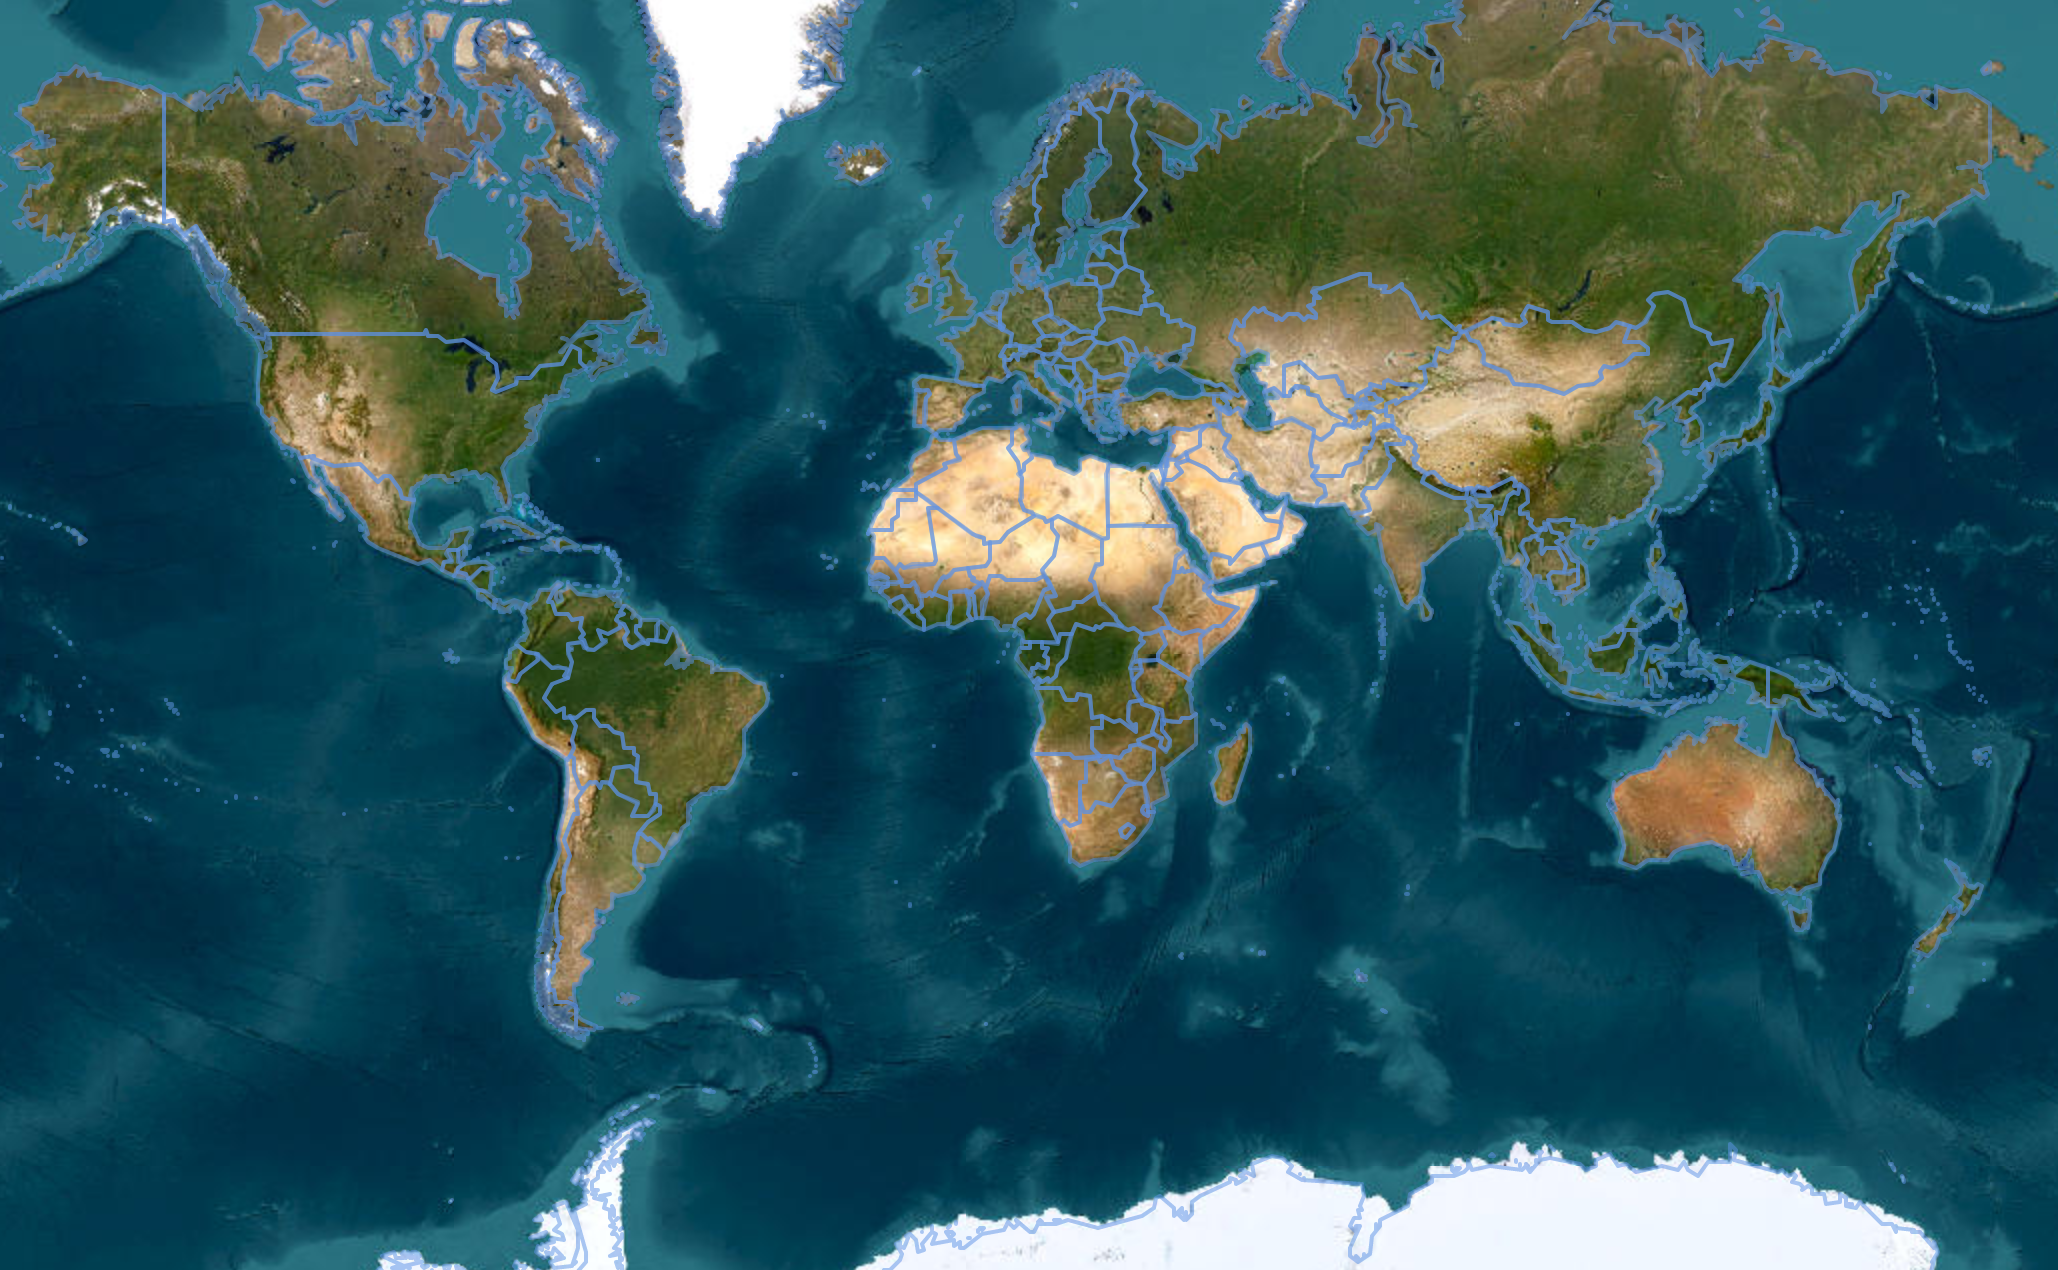
\includegraphics[width=0.5\textwidth,height=\textheight]{world.png}

}

\caption{\label{fig-world}Countries of the World}

\end{figure}%

\begin{quote}
``\ldots{} the particular and the universal are not to be seen as
opposites, \ldots{} the universal is not the negation of the particular
but is reached by a deeper exploration of the particular.'' (Cesaire in
UNESCO (1997))
\end{quote}

I use simulated data in this example. Data come from 30 hypothetical
countries. Data contain measures of a few key aspects of
parenting\footnote{I use the term parenting throughout this document,
  but am aware that such parenting may come from biological parents, or
  from other caregivers.} or caregiving that have proven salient in the
empirical literature on parenting to date: parental \texttt{warmth}, and
\texttt{physical\ punishment}. Both parenting measures are normally
distributed variables, and are considered to be \emph{Level 1}, or
\emph{individual level} variables. \texttt{group} is a hypothetical--and
somewhat arbitrary--group designation that could hypothetically refer to
something like different economic groups, or groups from different parts
of the country. \texttt{group} is also a \emph{Level 1} variable.

\texttt{HDI} is a measure of the \emph{Human Development Index} (United
Nations Development Program, 2022), and is measured at the \emph{country
level}, or \emph{Level 2}. (I discuss more in depth thinking about
levels of the data in Chapter~\ref{sec-conceptualframework}.)

Our \texttt{outcome} is conceptualized as a positive mental health
outcome or behavioral outcome, and higher levels of \texttt{outcome} are
considered to be better. Statistically, the data are clustered within
countries.

\begin{tcolorbox}[enhanced jigsaw, bottomrule=.15mm, breakable, title=\textcolor{quarto-callout-note-color}{\faInfo}\hspace{0.5em}{Download The Data in Stata Format}, colback=white, left=2mm, opacityback=0, coltitle=black, toptitle=1mm, bottomtitle=1mm, colframe=quarto-callout-note-color-frame, rightrule=.15mm, leftrule=.75mm, colbacktitle=quarto-callout-note-color!10!white, titlerule=0mm, toprule=.15mm, arc=.35mm, opacitybacktitle=0.6]

\begin{itemize}
\tightlist
\item
  \href{https://github.com/agrogan1/multilevel-thinking/raw/main/simulate-and-analyze-multilevel-data/simulated_multilevel_data.dta}{Cross-Sectional
  Data}
\item
  \href{https://github.com/agrogan1/multilevel-thinking/raw/main/simulate-and-analyze-multilevel-data/simulated_multilevel_longitudinal_data.dta}{Longitudinal
  Data}
\end{itemize}

\end{tcolorbox}

In this simulation, I construct the data so that \texttt{warmth} is
positively related to the \texttt{outcome}, while
\texttt{physical\ punishment} is negatively related to the
\texttt{outcome}.

\begin{longtable}[]{@{}
  >{\centering\arraybackslash}p{(\columnwidth - 12\tabcolsep) * \real{0.0833}}
  >{\centering\arraybackslash}p{(\columnwidth - 12\tabcolsep) * \real{0.1389}}
  >{\centering\arraybackslash}p{(\columnwidth - 12\tabcolsep) * \real{0.1250}}
  >{\centering\arraybackslash}p{(\columnwidth - 12\tabcolsep) * \real{0.3056}}
  >{\centering\arraybackslash}p{(\columnwidth - 12\tabcolsep) * \real{0.1111}}
  >{\centering\arraybackslash}p{(\columnwidth - 12\tabcolsep) * \real{0.0833}}
  >{\centering\arraybackslash}p{(\columnwidth - 12\tabcolsep) * \real{0.1389}}@{}}

\caption{\label{tbl-simulateddata}Simulated Multilevel Data}

\tabularnewline

\toprule\noalign{}
\begin{minipage}[b]{\linewidth}\centering
id
\end{minipage} & \begin{minipage}[b]{\linewidth}\centering
country
\end{minipage} & \begin{minipage}[b]{\linewidth}\centering
warmth
\end{minipage} & \begin{minipage}[b]{\linewidth}\centering
physical\_punishment
\end{minipage} & \begin{minipage}[b]{\linewidth}\centering
group
\end{minipage} & \begin{minipage}[b]{\linewidth}\centering
HDI
\end{minipage} & \begin{minipage}[b]{\linewidth}\centering
outcome
\end{minipage} \\
\midrule\noalign{}
\endhead
\bottomrule\noalign{}
\endlastfoot
1.1 & 1 & 3 & 2 & 2 & 69 & 59.18 \\
1.2 & 1 & 0 & 4 & 2 & 69 & 61.54 \\
1.3 & 1 & 4 & 4 & 1 & 69 & 51.87 \\
1.4 & 1 & 6 & 0 & 2 & 69 & 51.71 \\
1.5 & 1 & 2 & 3 & 2 & 69 & 55.88 \\
1.6 & 1 & 3 & 5 & 1 & 69 & 60.78 \\

\end{longtable}

\begin{figure}

\centering{

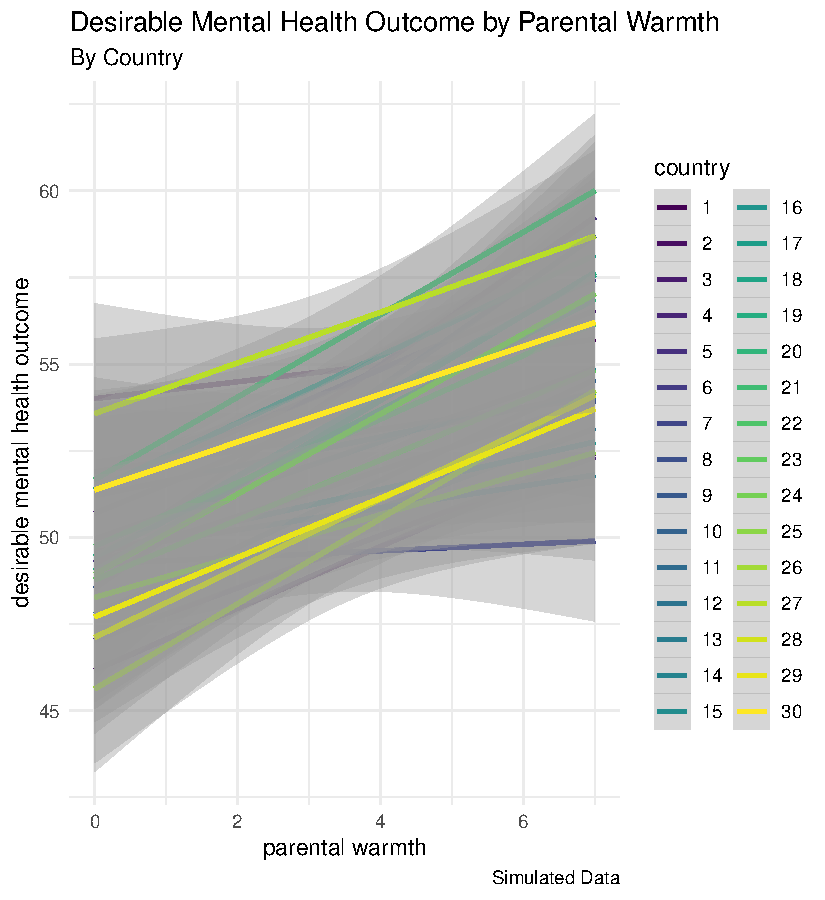
\includegraphics{simulated-multi-country-data_files/figure-pdf/fig-data-1.pdf}

}

\caption{\label{fig-data}Graph of Simulated Data}

\end{figure}%

\bookmarksetup{startatroot}

\chapter{Software}\label{sec-software}

\begin{quote}
``-- And so, why can't my numbers be beautiful to me? Why the scorn, the
doubt in your face? Do you think I am brittle and dusty as old paper?
Look again. See the numbers shine in my eyes.'' (Pye, 2011)
\end{quote}

In this document, I use Stata (StataCorp, 2021c) to analyze data. Stata
is my software of choice in this document because of Stata's overall
ease of use and intuitiveness. The creators of Stata have created a
powerful program that is extremely simple to use, but with a wide range
of both basic and advanced statistical capabilities.

The general idea of most Stata commands is:

\texttt{do\_something\ to\_a\_variable\_or\_variables,\ options}

Often it is not necessary to use any options since the authors of Stata
have done such a good job of thinking about the defaults.

For the sake of illustration, a few Stata commands are listed below.

\begin{longtable}[]{@{}ll@{}}
\caption{Example Stata Commands}\label{tbl-Statacommands}\tabularnewline
\toprule\noalign{}
Task & Command \\
\midrule\noalign{}
\endfirsthead
\toprule\noalign{}
Task & Command \\
\midrule\noalign{}
\endhead
\bottomrule\noalign{}
\endlastfoot
Open data & \texttt{use\ mydata.dta} \\
Descriptive statistics & \texttt{summarize\ x\ y} \\
Frequencies & \texttt{tabulate\ x} \\
Correlation & \texttt{corr\ x\ y} \\
Regression & \texttt{regress\ y\ x} \\
Logistic Regression & \texttt{logit\ y\ x,\ or} \footnote{Here we use
  the \texttt{,or} option to ask for \emph{odds ratios} instead of
  \emph{logit coefficients}.} \\
Multilevel Model &
\texttt{mixed\ y\ x\ \textbar{}\textbar{}\ group:\ x} \\
\end{longtable}

It is this multilevel syntax,
\texttt{mixed\ y\ x\ \textbar{}\textbar{}\ group:\ x} that we will be
using throughout this document.

\bookmarksetup{startatroot}

\chapter{Conceptual Framework}\label{sec-conceptualframework}

\begin{quote}
``Ubuntu'' defined as: ``A person is a person through other people.''
e.g.~in (Mangharam, 2017)
\end{quote}

\begin{quote}
``The language we have in that world is not large enough for the
territory that we've already entered.'' (Whyte \& Tippett, 2016)
\end{quote}

\section{Units of Analysis and Processes at Multiple
Levels}\label{units-of-analysis-and-processes-at-multiple-levels}

When confronted with multilevel data, one has a number of choices about
the units of analysis: one could consider individuals to be the units of
analysis; or, one could consider the larger social units to be the units
of analyses. With multilevel analytic methods, one is able to avoid this
false dichotomy, and to conceptualize the data from a multilevel
perspective, wherein both individuals and social units are different
levels of the same analysis. I discuss some of the statistical
implications of different ideas about the units of analysis in
Section~\ref{sec-wrongapproaches}.

Further, with multilevel models, we are not only able to consider the
idea of units of analysis at multiple levels of the data, but to
consider how variables at both Level 2 and Level 1 may affect an
individual level (Level 1) outcome.

\begin{figure}

\centering{

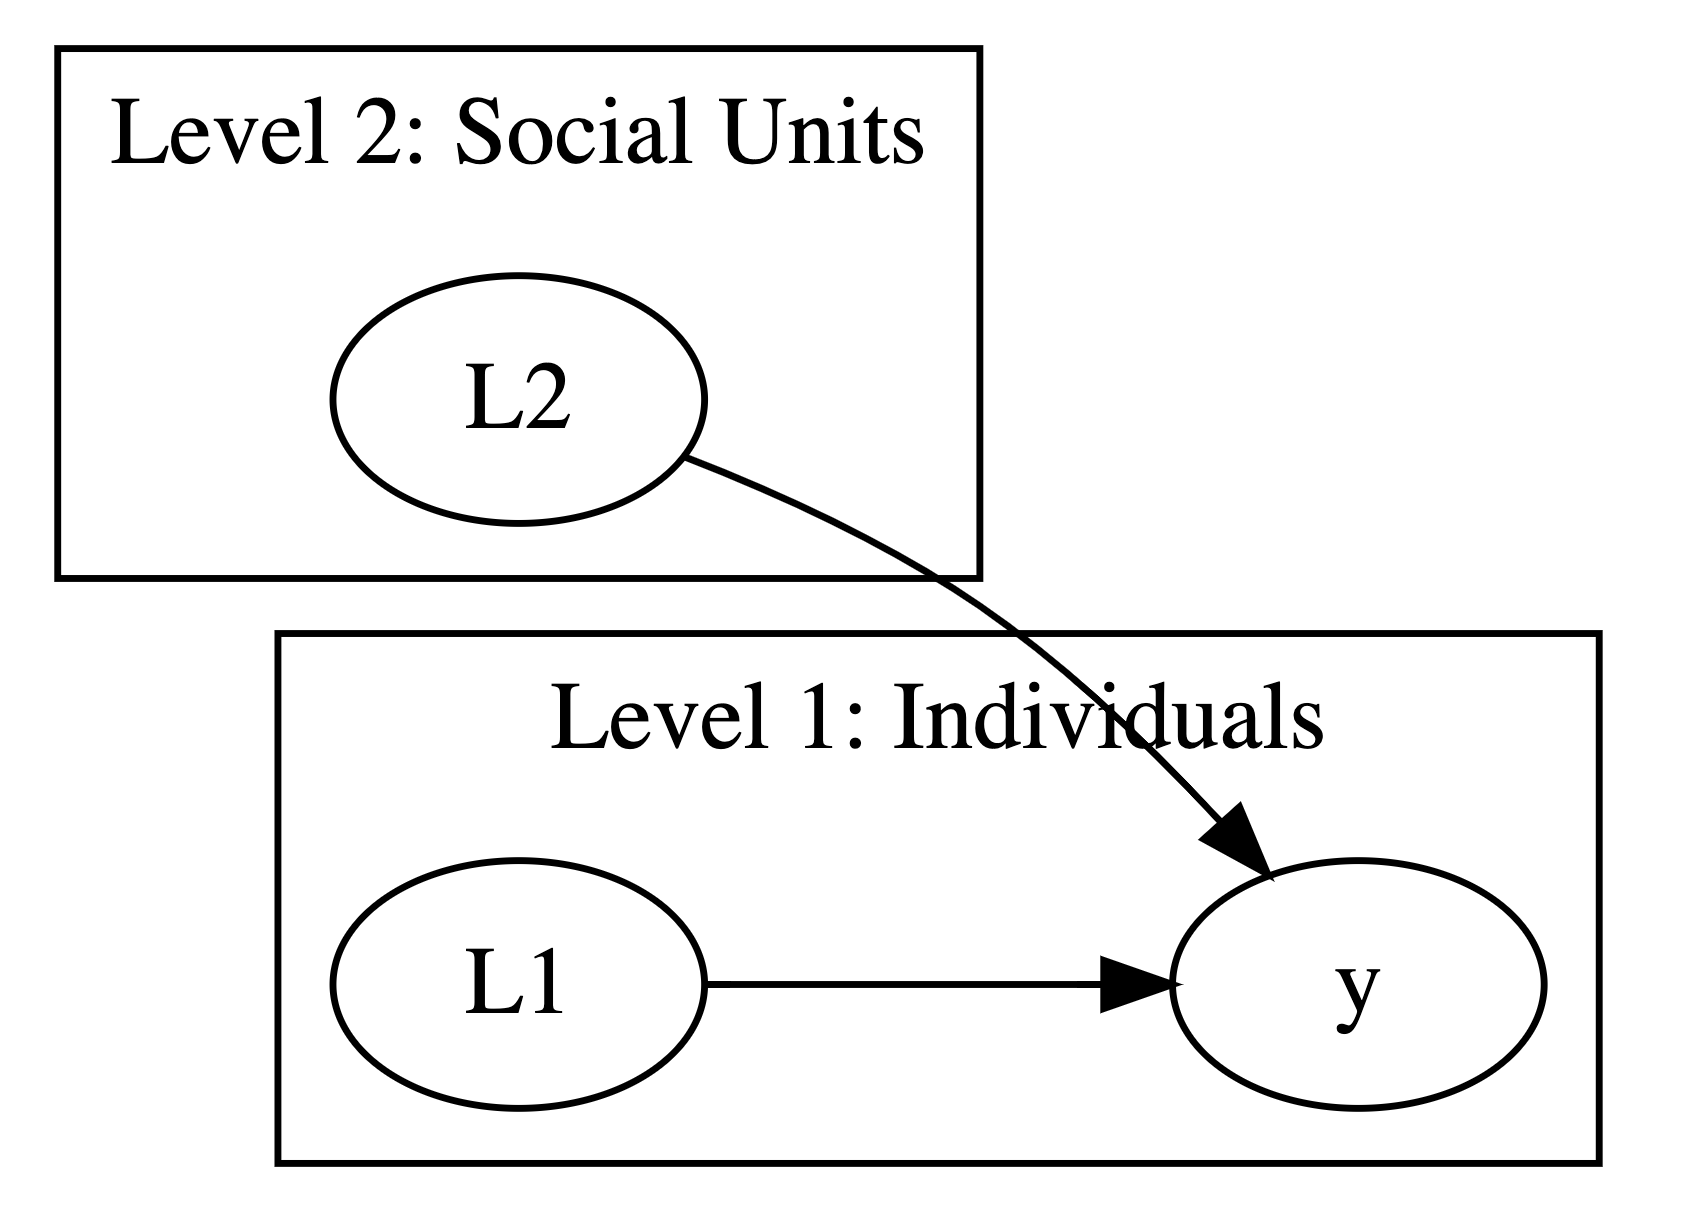
\includegraphics[width=0.5\textwidth,height=\textheight]{fig-conceptual.png}

}

\caption{\label{fig-conceptual}Conceptual Framework}

\end{figure}%

\section{Variables at Multiple Levels}\label{sec-levels}

In this document, I distinguish between \emph{conceptual} and
\emph{statistical} levels of variables.

By \emph{conceptual} level, I refer to whether a variable is
\emph{conceptualized} to be measure of an \emph{individual} level
characteristic, such as parenting or mental health, or a
\emph{community} level construct, such as community collective efficacy,
or community safety.

By \emph{statistical} level, I refer to whether a variable measures an
\emph{individual} response, or an \emph{aggregated} response.

\begin{longtable}[]{@{}
  >{\centering\arraybackslash}p{(\columnwidth - 4\tabcolsep) * \real{0.2436}}
  >{\centering\arraybackslash}p{(\columnwidth - 4\tabcolsep) * \real{0.3718}}
  >{\centering\arraybackslash}p{(\columnwidth - 4\tabcolsep) * \real{0.3846}}@{}}

\caption{\label{tbl-variablelevel}Multiple Levels of Variables}

\tabularnewline

\toprule\noalign{}
\begin{minipage}[b]{\linewidth}\centering
conceptual level
\end{minipage} & \begin{minipage}[b]{\linewidth}\centering
statistical level 1
\end{minipage} & \begin{minipage}[b]{\linewidth}\centering
statistical level 2
\end{minipage} \\
\midrule\noalign{}
\endhead
\bottomrule\noalign{}
\endlastfoot
1 & Individual response about parenting or mental health & Aggregated
responses about parenting or mental health \\
2 & Individual response about community & Aggregated response about
community \\
2 & N/A & Administrative indicator of social unit \\

\end{longtable}

\begin{itemize}
\item
  Thus, \(\text{mental health}_{ij}\) or \(\text{parenting}_{ij}\) would
  be considered in the terminology that I am using to be a variable both
  \emph{conceptually} and \emph{statistically} at Level 1.
\item
  \(\color{black}\overline{\text{mental health}_{.j}}\) or
  \(\color{black}\overline{\text{parenting}_{.j}}\) would be variables
  that \emph{conceptually} come from Level 1 responses, but are
  \emph{statistically} aggregated to Level 2.
\end{itemize}

\begin{quote}
Such aggregated variables represent the average level of a response
across each Level 2 unit. I could create such a level 2 variable for a
variable \texttt{x}, using the command:
\texttt{bysort\ group:\ egen\ mean\_x\ =\ mean(x)}. For example, in the
data described in Chapter~\ref{sec-simulateddata} I could create a mean
country level warmth score with the command
\texttt{bysort\ country:\ egen\ mean\_warmth\ =\ mean(warmth)}.
\end{quote}

\begin{itemize}
\item
  Using my terminology, \(\text{community collective efficacy}_{ij}\) or
  \(\text{community safety}_{ij}\) would be considered to be a variable
  that was \emph{conceptually} at Level 2, but \emph{statistically} at
  Level 1.
\item
  \(\color{black}\overline{\text{community collective efficacy}_{.j}}\)
  or \(\color{black}\overline{\text{community safety}_{.j}}\) would be
  variables that \emph{conceptually} refer to Level 2 concepts that are
  \emph{statistically} aggregated to Level 2.
\end{itemize}

Some variables only exist at Level 2, and their Level 1 counterparts are
undefined. For example, the size of a school, neighborhood, or country,
is inherently a Level 2 variable, with no easily definable Level 1
counterpart. Similarly, some administrative indicators, such as the Gini
level of inequality, while developed by calculating across Level 1
responses, have no easily definable Level 1 counterpart.

\section{Multilevel Models As The Study Of Variation and
Diversity}\label{sec-studyvariation}

Multilevel models are sometimes seen as an analytic technique that
\emph{controls for} the clustering or nesting of individuals inside
larger social units such as schools, neighborhoods, or countries. I will
describe below how this ability to \emph{control for} clustering is
indeed an important and crucial aspect of multilevel models.

However, my argument here is that multilevel models are better seen as a
method to \emph{explore} the variation and diversity inherent within
nested or clustered data. Again, while these issues are well understood
within the statistical literature (Kreft \& de Leeuw, 1998; Luke, 2004;
Rabe-Hesketh \& Skrondal, 2012; Raudenbush \& Bryk, 2002; Singer \&
Willett, 2003), they are less often noted in applied research.

\subsection{A First Example: A Study Of Parenting And Child
Development}\label{a-first-example-a-study-of-parenting-and-child-development}

In the graph below, imagine that physical punishment, or some other risk
factor, is associated with detrimental mental health outcomes. Each
country in the data has its own \emph{country specific regression line}.

\begin{figure}

\centering{

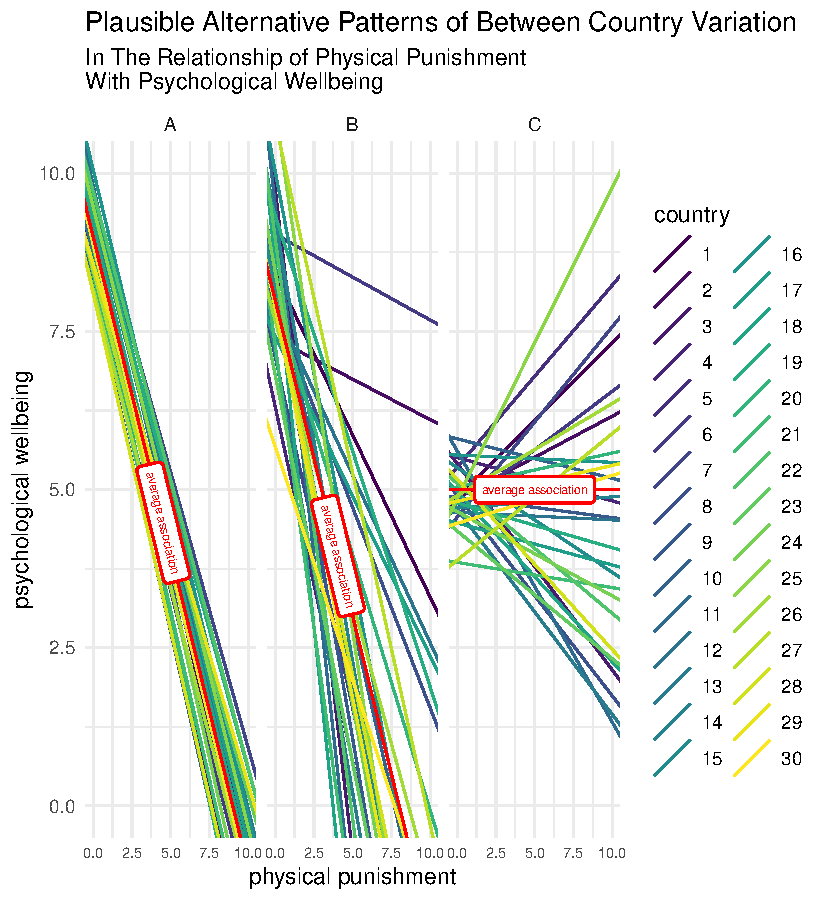
\includegraphics{conceptual-framework_files/figure-pdf/fig-variation1-1.pdf}

}

\caption{\label{fig-variation1}Plausible Alternative Patterns of Between
Country Variation}

\end{figure}%

In Panel A, there is some variation in the \emph{intercept}, which is
equivalent to saying that there is some variation in the average level
of psychological well-being across countries. When we look at the slope
of the country-specific regression lines in Panel A, we notice that
there is little variation in these \emph{slopes}. Put another way, there
is a great amount of consistency in the slopes of the country-specific
regression lines: parental use of physical punishment is consistently
associated with decreases in child psychological wellbeing across
countries.

In Panel B, the situation is different. There is more variation in the
\emph{intercept}, that is, more variation between countries in the
initial or average amount of psychological well-being. There is also
more variation in the \emph{slopes} of the country-specific regression
lines. While the average association between physical punishment and
psychological well-being is very similar to that in Panel A, there is
more variation across countries, in the relationship of physical
punishment and child psychological wellbeing, which would likely merit
exploration were one considering developing programs, policies or
interventions for different countries.

Lastly, the pattern of variation in Panel C is considerably different
from either Panel A or Panel B. The average association of physical
punishment with psychological well-being in the hypothetical scenario
represented by Panel C is approximately 0. There is some variation in
the \emph{intercepts} of the country-specific regression lines.
Additionally, there is considerable variation in the \emph{slopes} of
the country-specific regression line, suggesting that the use of
physical punishment might be beneficial in some countries, and
detrimental in others.

Empirically, data generally suggest a scenario somewhere between Panel A
and Panel B, but these different hypothetical scenarios afford us the
opportunity to think about possible patterns of variation.

\subsection{A Second Example: A Study Of A Treatment Or
Intervention}\label{a-second-example-a-study-of-a-treatment-or-intervention}

A second pedagogically helpful example might be obtained if we flip the
slopes in the diagram, and consider a different set of independent
variables, perhaps some kind of treatment or intervention designed to
improve psychological well-being.

\begin{figure}

\centering{

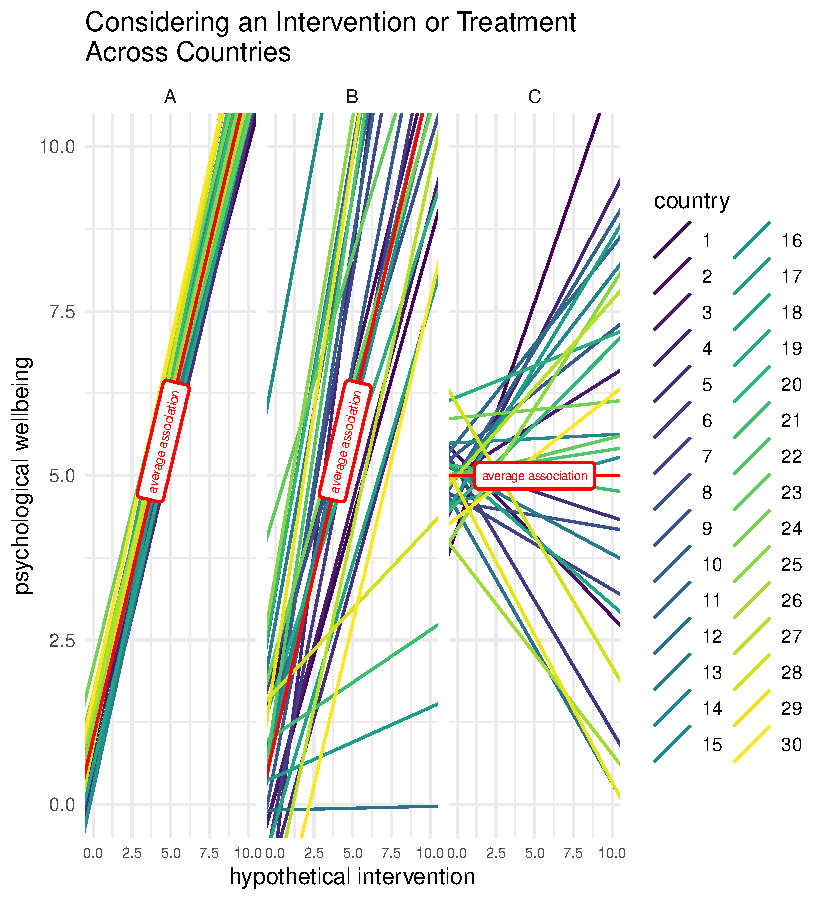
\includegraphics{conceptual-framework_files/figure-pdf/fig-variation2-1.pdf}

}

\caption{\label{fig-variation2}Considering an Intervention or Treatment
Across Countries}

\end{figure}%

We see a similar pattern as before, but the use of a different
substantive example may be illustrative.

In Panel A, there is relative consistency in the initial levels of
psychological well-being across countries, as well as consistency in the
degree to which the intervention is associated with improvements in
psychological well-being across countries.

In Panel B, we see more variation in both initial levels of
psychological well-being, but also more variation in the association of
the intervention with improvements in psychological well-being.

Lastly, in Panel C, we note an overall association of the intervention
with psychological well-being that is close to zero. However
associations vary widely by countries. In some countries there appears
to be evidence that the intervention is beneficial, while in other
countries there appears to be evidence that the intervention is not
beneficial, or even possibly harmful.

\subsection{Exploring Variation}\label{exploring-variation}

Thus, I emphasize an approach to multilevel modeling that sees
multilevel modeling as the \emph{study of variation}, not simply
\emph{accounting for variation}, or \emph{controlling for variation}.

\begin{quote}
``\ldots{} universal theorizing requires adequately sampled (i.e.,
diverse) data and better appreciation of issues of comparability and the
most powerful theories ought to predict and explain variation, not sweep
variation under the rug.'' (Blasi et al., 2022)
\end{quote}

Again, sophisticated treatments of all of the ideas are available in one
form or another across the excellent textbooks on multilevel modeling
(Kreft \& de Leeuw, 1998; Luke, 2004; Rabe-Hesketh \& Skrondal, 2012;
Raudenbush \& Bryk, 2002; Singer \& Willett, 2003). However, some of
these ideas appear less often in applied research, and my intention here
is to make the application of these ideas to applied research more
clear.

\bookmarksetup{startatroot}

\chapter{The Cross Sectional Multilevel
Model}\label{the-cross-sectional-multilevel-model}

\begin{quote}
``Mathematical Science shows us what is. It is the language of unseen
relations between things. But to use \& apply that language we must be
able fully to appreciate, to feel, to seize, the unseen, the
unconscious. Imagination too shows us what is, the is that is beyond the
senses.'' (Lovelace, 1992)
\end{quote}

I begin this chapter by introducing two key concepts: multilevel models
can improve our estimation of p values; multilevel models can improve
our estimation of \(\beta\) coefficients.

In these sections I make some initial use of the Stata syntax for
regression \texttt{regress\ y\ x\ z}, and the Stata syntax for
multilevel models,
\texttt{mixed\ y\ x\ z\ \textbar{}\textbar{}\ groupid:}.

After introducing these two key concepts of multilevel modeling, I then
begin a more in depth exploration of the equations and concepts and
statistical syntax of the cross sectional multilevel model.

\section{Estimating Standard Errors And p Values}\label{sec-pvalues}

\subsection{Introduction}\label{introduction-1}

If the data are grouped, nested, or clustered, then this aspect of the
structure of the data needs to be accounted for. Bland \& Altman (1994)
describe a simulation in which grouped data are artificially generated
according to the following procedure.

\begin{quote}
``The data were generated from random numbers, and there is no relation
between X and Y at all. Firstly, values of X and Y were generated for
each `subject,' then a further random number was added to make the
individual observation.'' (Bland \& Altman, 1994)
\end{quote}

The graph below illustrates the process of simulating the data.

\begin{figure}

\centering{

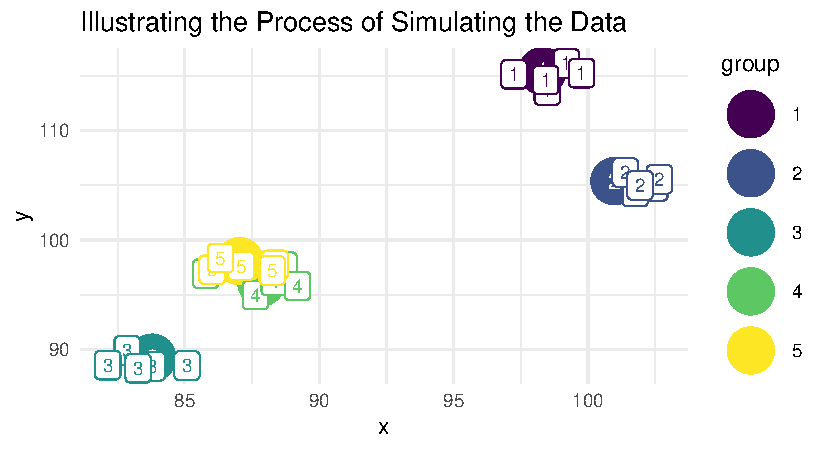
\includegraphics{cross-sectional_files/figure-pdf/fig-simulatedclustereddata-1.pdf}

}

\caption{\label{fig-simulatedclustereddata}Simulated Clustered Data}

\end{figure}%

\subsection{Compare OLS and MLM}\label{compare-ols-and-mlm}

An analysis that is not aware of the grouped nature of the data will
give biased results, will mis-estimate standard errors, and importantly,
will often attribute statistical significance to some of the independent
variables when this is not appropriate (Bland \& Altman, 1994;
Raudenbush \& Bryk, 2002).

In the example below, we compare a simple ordinary least squares
analysis of the data with a multilevel model that accounts for the
clustered nature of the data.

The Stata syntax that we use for each analysis is:

\begin{itemize}
\tightlist
\item
  OLS: \texttt{regress\ y\ x}
\item
  Multilevel Model: \texttt{mixed\ y\ x\ \textbar{}\textbar{}\ group:}
\end{itemize}

\begin{longtable}[]{@{}lllll@{}}
\toprule\noalign{}
& OLS & & MLM & \\
\midrule\noalign{}
\endhead
\bottomrule\noalign{}
\endlastfoot
x & 1.046 & ** & 0.039 & \\
Intercept & 4.488 & & 97.005 & ** \\
var(\_cons) & & & 74.523 & \\
var(e) & & & 0.594 & \\
Number of observations & 25 & & & \\
\end{longtable}

** p\textless.01, * p\textless.05

We see that in the ordinary least squares analysis, the independent
variable is judged to have a statistically significant association with
the dependent variable. The more appropriate multilevel model finds that
in fact the independent variable \(x\) is \emph{not} associated with
\(y\). Thus, the multilevel model provides more accurate results than
OLS in the presence of clustered data.

\section{Multilevel Structure}\label{sec-multilevelstructure}

Associations between two variables can be \emph{very different} (or even
\emph{reversed}) depending upon whether or not the analysis is ``aware''
of the grouped, nested, or clustered nature of the data (Gelman et al.,
2007). In the example presented here, the groups are countries, but
could as easily be neighborhoods, communities, or schools.

\begin{quote}
For teaching purposes, I use an example with very few clusters, although
it would be more appropriate to apply multilevel analysis to an example
with many more clusters e.g.~(\(N_\text{clusters} >= 30\))
\end{quote}

A model that is ``aware'' of the clustered nature of the data may
provide very different--likely better--substantive conclusions than a
model that is not aware of the clustered nature of the data.

I use some data simulated for this particular example.

\subsection{Graphs}\label{graphs}

\subsubsection{A ``Naive'' Graph}\label{a-naive-graph}

This ``naive'' graph is unaware of the grouped nature of the data.
Notice that the overall regression line slopes downward, even though
there is some suggestion that \emph{within each group} the regression
lines may slope upward.

\begin{figure}

\centering{

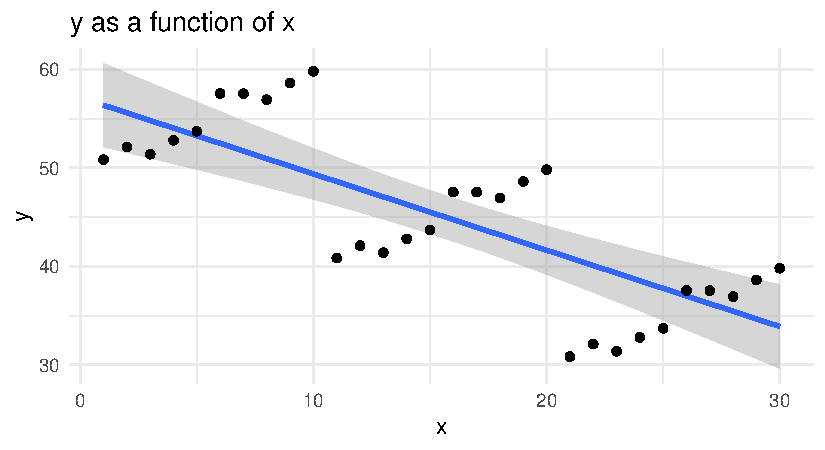
\includegraphics{cross-sectional_files/figure-pdf/fig-naive-1.pdf}

}

\caption{\label{fig-naive}A `Naive' Graph}

\end{figure}%

\subsubsection{An ``Aware'' Graph}\label{an-aware-graph}

This ``aware'' graph is aware of the grouped nature of the data. The
graph is ``aware'' of the grouped or clustered nature of the data, and
provides indication that the regression lines \emph{when accounting for
group} slope upward.

\begin{figure}

\centering{

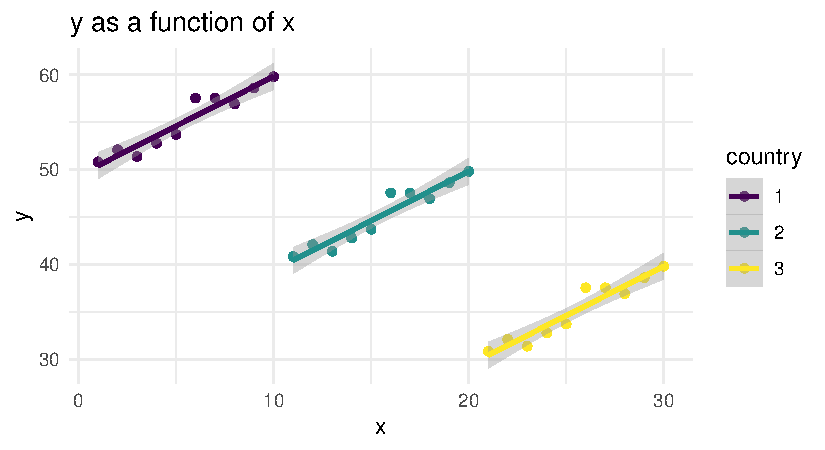
\includegraphics{cross-sectional_files/figure-pdf/fig-aware-1.pdf}

}

\caption{\label{fig-aware}An `Aware' Graph}

\end{figure}%

\subsection{Regressions}\label{regressions}

\subsubsection{A ``Naive'' OLS Analysis vs.~An ``Aware'' MLM
Analysis}\label{a-naive-ols-analysis-vs.-an-aware-mlm-analysis}

The Stata syntax that we use for these analyses is:

\begin{itemize}
\tightlist
\item
  OLS: \texttt{regress\ y\ x}
\item
  Multilevel Model: \texttt{mixed\ y\ x\ \textbar{}\textbar{}\ country:}
\end{itemize}

The OLS model with only \emph{x} as a covariate is not aware of the
grouped structure of the data, and the coefficient for \emph{x} in the
OLS model reflects this. The coefficient for \emph{x} in the OLS model
is \emph{negative}, and statistically significant.

The multilevel model is aware of the grouped structure of the data, and
the coefficient for \emph{x} in the multilevel model reflects this. The
coefficient for \emph{x} in the multilevel model is \emph{positive}, and
statistically significant.

\begin{longtable}[]{@{}lllll@{}}
\toprule\noalign{}
& OLS & & MLM & \\
\midrule\noalign{}
\endhead
\bottomrule\noalign{}
\endlastfoot
x & -0.775 & ** & 1.038 & ** \\
Intercept & 57.133 & ** & 29.029 & ** \\
var(\_cons) & & & 276.867 & \\
var(e) & & & 0.916 & \\
Number of observations & 30 & & & \\
\end{longtable}

** p\textless.01, * p\textless.05

\subsection{A Thought Experiment}\label{a-thought-experiment}

When might a situation like this arise in practice? This is surprisingly
difficult to think through.

Imagine that \emph{x} is a protective factor, or an intervention or
treatment. Imagine that \emph{y} is a desirable outcome, like improved
mental health or psychological well being.

Now imagine that residents of countries provide more of the protective
factor or more of the intervention in situations where there are lower
levels of the desirable outcome. If one thinks about it, this is a very
plausible situation.

\begin{quote}
A naive analysis that was unaware of the grouped nature of the data
would therefore misconstrue the results, suggesting that the
intervention was harmful, when it was in fact helpful.
\end{quote}

\begin{figure}[H]

{\centering 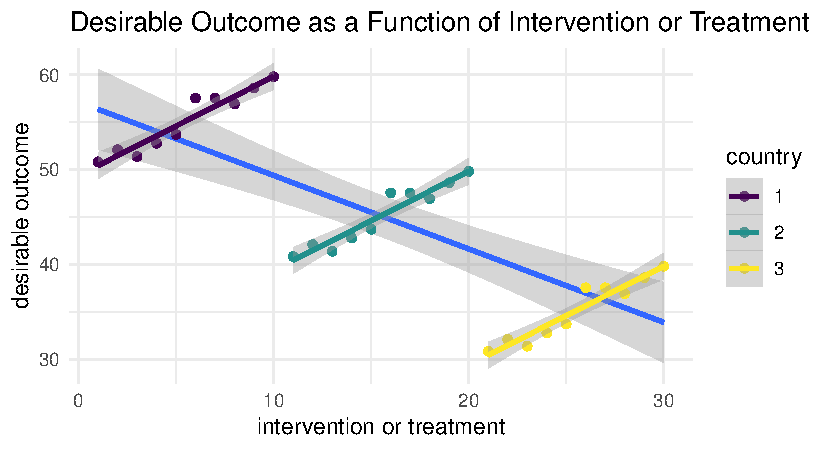
\includegraphics{cross-sectional_files/figure-pdf/unnamed-chunk-9-1.pdf}

}

\caption{A Heuristic Example}

\end{figure}%

The idea that group level and individual level relationships must be the
same (Firebaugh, 2001) has been termed the ``ecological fallacy''.

These data are constructed to provide this kind of extreme example, but
it easy to see how multilevel thinking, and multilevel analysis may
provide better answers than one would get if one ignored the grouped
nature of the data.

\section{The Equation}\label{the-equation}

The equation for the multilevel model can be written in several ways: as
multiple levels of equations; or as a single equation. The advantage of
having multiple levels of equations is that these multiple equations
make clear the multiple levels of the data, and thus conform to an
initial understanding of how a multilevel model should be estimated.
However, \emph{results} from multiple levels of equations quickly become
difficult to interpret, and thus, I will not spend a great deal of time
on discussing empirical results of the two level formulation. Whether
multiple levels of equations, or a single equation are employed, the
numerical results are equivalent.s

\subsection{Two Levels of Equations}\label{two-levels-of-equations}

I start with two levels of equations: Level 1 at the level of the
individual; and Level 2 at the level of the country.

\subsubsection{Level 1 (Individuals)}\label{level-1-individuals}

\begin{equation}\phantomsection\label{eq-MLM1}{y_{ij} = \beta_{0j} + \beta_{1j} x_{ij} + \beta_{2j} z_{ij} + e_{ij}}\end{equation}

\subsubsection{Level 2 (Countries)}\label{level-2-countries}

\begin{equation}\phantomsection\label{eq-MLM2}{\beta_{0j} = \gamma_{00} +\gamma_{01} w_j + u_{0j}}\end{equation}

\[\beta_{1j} = \gamma_{10} + u_{1j}\]

\[\beta_{2j} = \gamma_{20}\]

\[\beta_{3j} = \gamma_{30}\]

Here \(y_{ij}\) is the dependent variable, or outcome for the model. We
note that the \(ij\) subscripts indicate that this is outcome \(y\) for
individual \(i\) in country \(j\). Note that the outcome is at Level 1,
or the level of individuals. \(\beta_{0j}\) is a regression intercept,
and the other \(\beta\)'s\footnote{Technically, all of these \(\beta\)'s
  could be written as \(\beta_j\) since the multilevel model could be
  said to estimate a regression parameter for each group, in this case
  each country. One could even write \(\beta_{jk}\) to represent the
  regression parameter for the \(k^{th}\) independent variable the for
  the \(j^{th}\) group or country. To keep matters simple, I simply
  write \(\beta\) in most cases.} are regression slope parameters.
\(x_{ij}\) and \(z_{ij}\) are independent variables and \(t_{ij}\) is an
independent variable indicating the time at which different data points
are measured. I note that in this discussion I am \emph{not} considering
a model in which there are repeated observations on the same
individuals, although the multilevel model is certainly extensible to
such cases. \(u_{0j}\) is a random intercept for the \(\beta_{0j}\)
term, and \(u_{1j}\) is a random slope for the \(\beta_{1j}\) term,
indicating that we are modeling cross country variation in these
parameters. The other \(\beta\) terms are not modeled as having random
country level variation, although this could certainly be a possibility
in subsequent models.

In this formulation of the multilevel model, each regression parameter
\(\beta\) in the level 1 equation is the outcome of an equation at Level
2. The parameters for the Level 2 equations are represented by
\(\gamma\)'s. \(w\) a Level 2 variable appears in the first Level 2
equation.

\subsection{One Level of Equations}\label{one-level-of-equations}

By simply substituting the values of the Level 2 equations into the
Level 1 equations--and rewriting the \(\gamma\)'s as \(\beta\)'s--we
obtain:

\begin{equation}\phantomsection\label{eq-MLM}{y_{ij} = \beta_0 + \beta_1 x_{ij} + \beta_2 z_{ij} + \beta_3 w_{j} + u_{0j} + u_{1j} \times x + e_{ij}}\end{equation}

Here again \(y_{ij}\) is the dependent variable, or outcome for the
model. \(\beta_0\) is a regression intercept, and the \(\beta\)'s are
regression parameters. \(x_{ij}\) and \(z_{ij}\) are independent
variables and \(w\) is a Level 2 variable.

\begin{quote}
Notice that in this \emph{single equation} format all variables--no
matter their \emph{level}--appear in the same equation.
\end{quote}

In this formulation of the equation, the nature of the random effects is
more clear, and merits discussion. Notice that we have included a
\emph{random intercept} \(u_{0j}\) as well as a \emph{random slope}
\(u_{1j} \times x\). The \emph{random intercept}, \(u_{0j}\), indicates
that there is variation in the \emph{intercept} of the country specific
regression lines, as is true in Figure~\ref{fig-data}. The \emph{random
slope} term associated with \(x\), \(u_{1j} \times x\), indicates that
we are allowing for the possibility of variation in the \emph{slope} of
the regression lines that is associated with \(x\), in this case, the
slope of parental warmth, as is possibly suggested in
Figure~\ref{fig-data}.

To make these ideas more concrete, I rewrite this equation in terms of
the main substantive ideas of this document:

\[\text{outcome}_{ij} = \beta_0 + \beta_1 \text{parental warmth}_{ij} + \\ \beta_2 \text{physical punishment}_{ij} +\]
\[\beta_3 \text{group}_{ij} + \beta_4 \text{HDI}_{j} + \]
\begin{equation}\phantomsection\label{eq-MLMsubstantive}{u_{0j} + u_{1j} \times \text{parental warmth} + e_{ij}}\end{equation}

Put substantively, this model indicates that the outcome can be
conceptualized as a function of an intercept term, and contributions of
parental warmth, physical punishment, group membership, and country
level HDI. The random intercept, \(u_{0j}\) indicates that there is some
unexplained variation in the outcome at the country level. The random
slope \(u_{1j} \times \text{parental warmth}\) indicates that the model
is allowing for country level variation in the association of parental
warmth with the outcome. Inspection of Figure~\ref{fig-data} indicates
that it might be possible that there would be variation across countries
in this slope. The model could be extended to allow for country level
variation in other slope terms by adding other random slopes, eg
\(u_{2j}\), \(u_{3j}\), etc.

Drawing upon ideas from Chapter~\ref{sec-software}, this single level
equation can be easily represented in Stata syntax.

\begin{Shaded}
\begin{Highlighting}[]

\NormalTok{mixed outcome warmth physical\_punishment }\FunctionTok{group}\NormalTok{ HDI || country: warmth}
\end{Highlighting}
\end{Shaded}

\section{Regression With Simulated Multi-Country
Data}\label{sec-regression}

After considering some of these broader issues, let's now examine the
results of a multilevel regression with the simulated multicountry data.
I will again imagine that the desirable outcome is an outcome such as
improved psychological wellbeing.

\subsection{Unconditional Model}\label{sec-unconditional}

The unconditional model is a model with no \(x\)'s or covariates
(Raudenbush \& Bryk, 2002).

\begin{equation}\phantomsection\label{eq-unconditional}{\text{outcome}_{ij} = \beta_0 + u_{0j} + e_{ij}}\end{equation}

Here, \(\text{outcome}_{ij}\) is a function of an intercept \(\beta_0\),
a country specific error term, \(u_{0j}\), and an individual level error
term \(e_{ij}\).

Thus, all of the variation in \(\text{outcome}_{ij}\) is--given the
\emph{unconditional} nature of our model--attributable to unmeasured
variation at the country and individual level.

\subsection{Intra-Class Correlation Coefficient}\label{sec-ICC}

I now introduce a measure known as the Intra-Class Correlation
Coefficient, (ICC) that can be computed from this unconditional model
(Raudenbush \& Bryk, 2002).

\begin{equation}\phantomsection\label{eq-ICC}{\text{ICC} = \frac{var(u_{0j})}{var(u_{0j}) + var(e_{ij})}}\end{equation}

Heuristically:

\begin{equation}\phantomsection\label{eq-ICCheuristic}{\text{ICC} = \frac{\text{group level variation}}{\text{group level variation} + \text{individual level variation}}}\end{equation}

The ICC from the \emph{unconditional} model
(Equation~\ref{eq-unconditional}) is the most informative ICC as it
represents the amount of variation in the dependent variable that could
\emph{potentially} be explained by the grouping variable.

The Stata syntax that we use is:

\begin{Shaded}
\begin{Highlighting}[]

\NormalTok{mixed outcome || country: }

\KeywordTok{estat}\NormalTok{ icc}
\end{Highlighting}
\end{Shaded}

\begin{longtable}[]{@{}lll@{}}
\toprule\noalign{}
& cross\_sectional0 & \\
\midrule\noalign{}
\endhead
\bottomrule\noalign{}
\endlastfoot
\_cons & 53.468 & ** \\
var(\_cons) & 3.349 & \\
var(e) & 40.883 & \\
\end{longtable}

** p\textless.01, * p\textless.05

From \texttt{estat\ icc}, or calculating by hand, we see that the ICC
for this data is .076 or 7.6\%.

As we add covariates, \(x\)'s, to the model the ICC will most often
decrease.

\subsection{Conditional Model}\label{conditional-model}

We next estimate a \emph{conditional} model, \emph{with} independent
variables.

The Stata syntax that we use is:

\begin{Shaded}
\begin{Highlighting}[]

\NormalTok{mixed outcome warmth physical\_punishment }\FunctionTok{group}\NormalTok{ HDI || country: warmth}
\end{Highlighting}
\end{Shaded}

\begin{longtable}[]{@{}lll@{}}
\toprule\noalign{}
& cross\_sectional & \\
\midrule\noalign{}
\endhead
\bottomrule\noalign{}
\endlastfoot
warmth & 0.962 & ** \\
physical\_punishment & -0.845 & ** \\
group & & \\
2 & 1.084 & ** \\
HDI & 0.011 & \\
\_cons & 50.964 & ** \\
var(warmth) & 0.000 & \\
var(\_cons) & 3.370 & \\
var(e) & 36.019 & \\
\end{longtable}

** p\textless.01, * p\textless.05

The data suggest that parental warmth is positively associated with the
desirable outcome, and that this result is statistically significant.
Parental use of physical punishment is associated with statistically
significant decreases in the desirable outcome. I note that there is
some variation in the \emph{constant} indicating that there is some
variation in the initial or average levels of the desirable
outcome--again improved psychological well-being--that is attributable
to country.

There is--in contrast--no discernible variation in the \emph{slope}
associated with parental warmth that is attributable to country. Thus,
the relationship of parental warmth with child outcomes does not appear
to differ appreciably from country to country.

\texttt{HDI}, the \emph{Human Development Index}, our only country
level, or Level 2, variable in this model is not associated with the
outcome.

\section{Correlation of Random Intercept and Random
Slope(s)}\label{correlation-of-random-intercept-and-random-slopes}

One could also consider a situation in which a random slope or slopes
were correlated with each other, and with the random intercept. In the
equation that we are considering, this would entail estimation of
whether or not, the random intercept, \(u_{0j}\), was correlated with
the random slope for warmth, \(u_{1j}\).

Substantively, this question would be asking whether the association of
warmth and the outcome, was correlated with the initial level or average
level of the outcome. From Figure~\ref{fig-data}, it appears that there
is some slight evidence that the country specific regression slopes are
more steep in countries where the initial level of the outcome is
higher. However, we may wish to investigate this question more
rigorously.

By default, Stata estimates models, where the random slope or slopes are
uncorrelated with each other, and uncorrelated with the intercept
(StataCorp, 2021b). We see this in Equation~\ref{eq-varcovar} below,
where the diagonal elements are the \emph{variances} of each of the
random effects, and the off diagonals, which would be the
\emph{covariances} of the random effects are constrained to 0.

\begin{equation}\phantomsection\label{eq-varcovar}{\begin{bmatrix}
var(u_{0j}) & 0 \\
0 & var(u_{1j}) 
\end{bmatrix}}\end{equation}

Within Stata, we can ask to allow such a correlation with the
\texttt{cov(uns)} option.

\begin{equation}\phantomsection\label{eq-varcovaruns}{\begin{bmatrix}
var(u_{0j}) & cov(u_{0j}, u_{1j}) \\
cov(u_{0j}, u_{1j}) & var(u_{1j}) 
\end{bmatrix}}\end{equation}

We use the following syntax.

\begin{Shaded}
\begin{Highlighting}[]

\NormalTok{mixed outcome warmth physical\_punishment }\FunctionTok{group}\NormalTok{ HDI || country: warmth, cov(uns)}
\end{Highlighting}
\end{Shaded}

When we estimate such a model, we get the following information.

\begin{longtable}[]{@{}lll@{}}
\toprule\noalign{}
& cross\_sectional2 & \\
\midrule\noalign{}
\endhead
\bottomrule\noalign{}
\endlastfoot
warmth & 0.962 & ** \\
physical\_punishment & -0.845 & ** \\
group & & \\
2 & 1.085 & ** \\
HDI & 0.010 & \\
\_cons & 50.987 & ** \\
var(warmth) & 0.000 & \\
var(\_cons) & 3.237 & \\
cov(warmth,\_cons) & 0.019 & \\
var(e) & 36.019 & \\
\end{longtable}

** p\textless.01, * p\textless.05

Results are mostly similar to those above. However, here, we are asking
additionally for information about the possible correlation of country
specific initial levels of the outcome and the slope of the country
specific regression line for parental warmth. Results indicate that
there is no reason to be believe that these two parameters are
correlated. Put more intuitively, it does not appear that parental
warmth is any more or less correlated with the outcome in countries
where initial levels of the outcome are higher.

\section{Within and Between}\label{sec-withinbetween}

Coefficients in models can be divided into within and between. A
substantive example may be helpful here. When we consider the variable
of parental \texttt{warmth}, we can imagine the parental warmth
expressed in each family, \(\text{warmth}_{ij}\), representing family
\emph{i} in country \emph{j}. We can also think about the \emph{grand
mean} of warmth across the entire sample,
\(\overline{\text{warmth}}_{..}\). We can then also think about the mean
expression of parental warmth in each country,
\(\overline{\text{warmth}}_{.j}\), i.e.~the mean level of parental
warmth in country \emph{j}.

\begin{figure}

\centering{

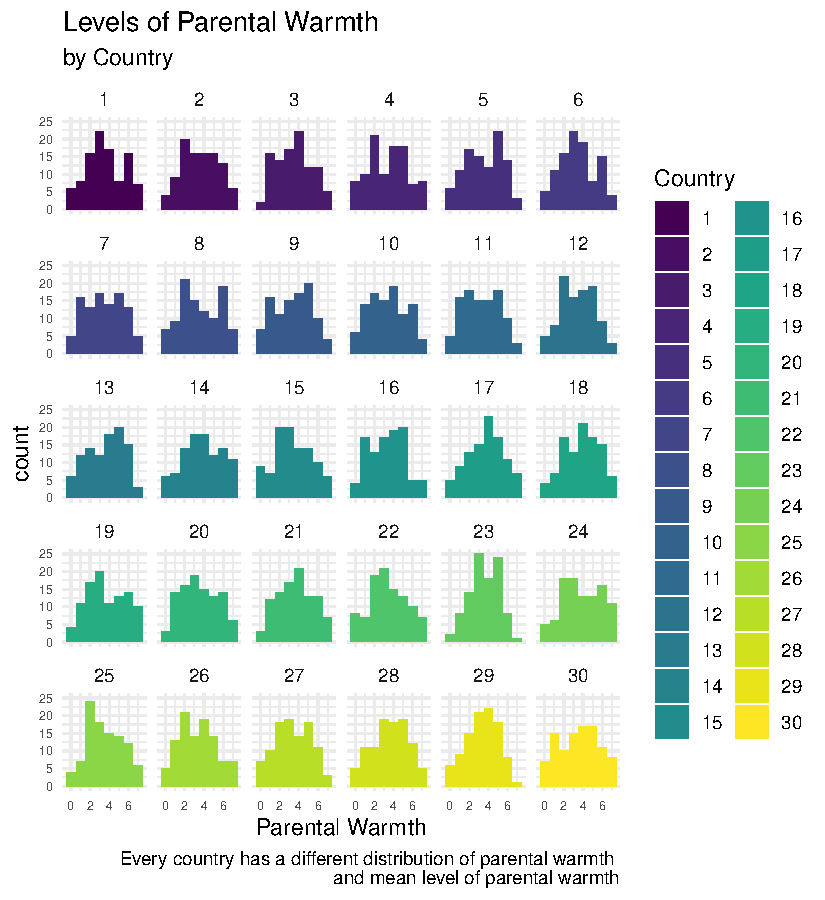
\includegraphics{cross-sectional_files/figure-pdf/fig-distributionwarmth-1.pdf}

}

\caption{\label{fig-distributionwarmth}Distribution of Parental Warmth
Across Countries}

\end{figure}%

Bearing this in mind, one can then think about the \emph{difference}
between each individual expression of parental warmth and the overall,
or grand mean: \(\text{warmth}_{ij} - \overline{\text{warmth}}_{..}\).
This value can then be decomposed into two values:

\[\text{warmth}_{ij} - \overline{\text{warmth}}_{..} = \text{warmth}_{ij} - \overline{\text{warmth}}_{.j} + \overline{\text{warmth}}_{.j} - \overline{\text{warmth}}_{..}\]
Put into words, this equation says that the difference in parental
warmth displayed by family i in country j from the overall or grand mean
of parental warmth is composed of two components:

\begin{itemize}
\tightlist
\item
  \emph{Within Country Component}: How is the level of warmth expressed
  by family \emph{i} in country \emph{j} different from the \emph{mean}
  level of warmth in country \emph{j}. Is family \emph{i} different from
  the \emph{average} family in country \emph{j}? For this particular
  country, is this a family that is higher, or lower, than average in
  parental warmth?
\item
  \emph{Between Country Component}: How is the \emph{mean} level of
  warmth in country \emph{j} different from the overall or \emph{grand
  mean} level of warmth in the sample as a whole? To what degree is
  country \emph{j} different from \emph{all countries} in the sample? Is
  this country a country where parents tend to be higher, or lower, in
  parental warmth?
\end{itemize}

Theoretically, or conceptually, one might imagine that it would be
useful to decompose a particular behavior into within country and
between country components. The within country component could be
theorized as \emph{how an individual family differs from their context},
and the between country component could be theorized as \emph{how a
particular context differs from the average context}.

\begin{figure}

\centering{

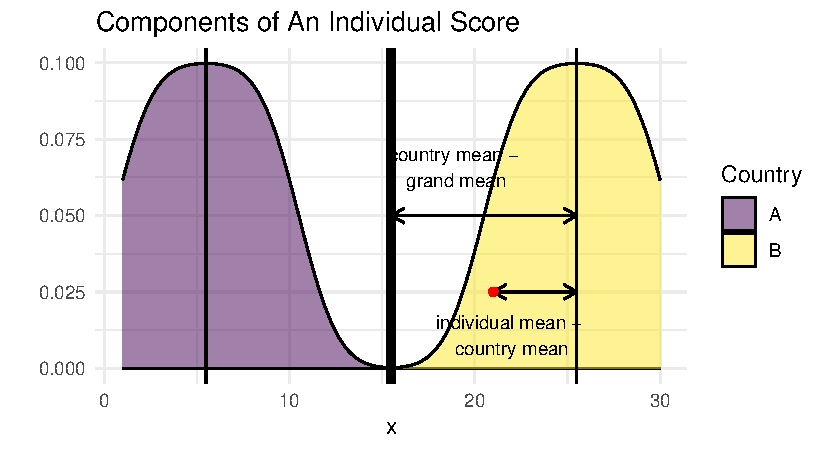
\includegraphics{cross-sectional_files/figure-pdf/fig-withinbetween-1.pdf}

}

\caption{\label{fig-withinbetween}Decomposing a Variable into Within and
Between Differences}

\end{figure}%

In terms of using statistical software (Stata), we need to follow a few
steps.

\begin{enumerate}
\def\labelenumi{\arabic{enumi}.}
\tightlist
\item
  Calculate the \emph{grand mean} of the variable.
\end{enumerate}

\begin{Shaded}
\begin{Highlighting}[]

\KeywordTok{egen}\NormalTok{ gmean\_warmth = }\KeywordTok{mean}\NormalTok{(warmth)}
\end{Highlighting}
\end{Shaded}

\begin{enumerate}
\def\labelenumi{\arabic{enumi}.}
\setcounter{enumi}{1}
\tightlist
\item
  Calculate \emph{country specific means} of the variable.
\end{enumerate}

\begin{Shaded}
\begin{Highlighting}[]

\KeywordTok{bysort}\NormalTok{ country: }\KeywordTok{egen}\NormalTok{ cmean\_warmth = }\KeywordTok{mean}\NormalTok{(warmth)}
\end{Highlighting}
\end{Shaded}

\begin{enumerate}
\def\labelenumi{\arabic{enumi}.}
\setcounter{enumi}{2}
\tightlist
\item
  Calculate:

  \begin{itemize}
  \tightlist
  \item
    individual scores - country specific means
  \item
    country specific means - grand mean
  \end{itemize}
\end{enumerate}

\begin{Shaded}
\begin{Highlighting}[]

\KeywordTok{generate}\NormalTok{ dev\_warmth = warmth {-} cmean\_warmth}

\KeywordTok{generate}\NormalTok{ cdev\_warmth = cmean\_warmth {-} gmean\_warmth}
\end{Highlighting}
\end{Shaded}

\begin{enumerate}
\def\labelenumi{\arabic{enumi}.}
\setcounter{enumi}{3}
\tightlist
\item
  Estimate the model with within and between.
\end{enumerate}

\begin{Shaded}
\begin{Highlighting}[]

\NormalTok{mixed outcome dev\_warmth cdev\_warmth physical\_punishment i.}\FunctionTok{group}\NormalTok{ HDI }\CommentTok{///}
\NormalTok{|| country: warmth}
\end{Highlighting}
\end{Shaded}

\begin{longtable}[]{@{}lll@{}}
\toprule\noalign{}
& cross\_sectional3 & \\
\midrule\noalign{}
\endhead
\bottomrule\noalign{}
\endlastfoot
dev\_warmth & 0.961 & ** \\
cdev\_warmth & 1.899 & \\
physical\_punishment & -0.845 & ** \\
group & & \\
2 & 1.085 & ** \\
HDI & 0.008 & \\
\_cons & 54.489 & ** \\
var(warmth) & 0.000 & \\
var(\_cons) & 3.351 & \\
var(e) & 36.019 & \\
\end{longtable}

** p\textless.01, * p\textless.05

Estimates suggest that both the difference in an individual family's
expression of parental warmth from the country level mean, \emph{but
not} the difference in the country level mean from the grand mean are
statistically significant predictors of the outcome.

\section{Summary of Advantages Of The Multilevel
Model}\label{summary-of-advantages-of-the-multilevel-model}

The discussion so far gives an idea of the advantages of the multilevel
model for studying intrinsically multilevel data: children in classrooms
or schools; individuals or families in neighborhoods; individuals or
families in countries. These advantages can be summarized below:

\begin{enumerate}
\def\labelenumi{\arabic{enumi}.}
\tightlist
\item
  Standard errors are estimated correctly as is statistical
  significance. This means that p values are correctly estimated
  accounting for the clustered or nested nature of the data. More
  colloquially, this most often means that we do not make the mistake of
  attributing statistical significance to a given risk or protective
  factor, when such a statistical significance is not warranted. Put
  even more straightforwardly correct estimation of standard errors and
  statistical significance prevents us from seeing results that are
  simply not present in the data, whether those concern risk factors or
  protective factors.
\item
  Regression coefficients are estimated correctly accounting for the
  clustered or nested structure of the data. If one does not account for
  the clustered or nested structure of the data, regression slopes can
  be estimated as negative when they are more correctly estimated as
  positive, or as null, or conversely estimated as positive when there
  are more correctly seen as negative (or null). Again, to phrase things
  in a more colloquial fashion, this means that we do not judge
  something to be a risk factor when it is in fact a protective factor
  or a null effect; or a protective factor when it is in fact a risk
  factor, or a null effect.
\end{enumerate}

\section{Some Wrong (or Partially Wrong)
Approaches}\label{sec-wrongapproaches}

When data are clustered--e.g.~residents in neighborhoods, children in
schools, families in countries--it is worth discussing the fact that we
have several choices statistically as how to proceed, other than using a
multilevel model. Given the discussion so far, we can see the advantages
of a multilevel model over these other approaches:

\begin{enumerate}
\def\labelenumi{\arabic{enumi}.}
\tightlist
\item
  First, we could simply ignore the clustering, and treat the data as
  though it were composed of statistically independent individuals,
  i.e.~statistically independent \(e_i\). As we have discussed above,
  however, this approach has at least two disadvantages. First, as
  discussed in Section~\ref{sec-pvalues}, this approach will
  mis-estimate standard errors, most often underestimating them,
  resulting in underestimated p values and false positives. Second, as
  discussed in Section~\ref{sec-multilevelstructure} ignoring clustering
  runs the risk of estimating regression \(\beta\)'s that are not
  estimated with information about the multilevel structure of the data,
  with the possibility that \(\beta\) coefficients may not only have
  incorrect statistical significance, but also incorrect magnitude, and
  even incorrect sign.
\item
  A second approach would be to \emph{aggregate} the data to the level
  of the higher social unit, e.g.~aggregating the data at the level of
  the neighborhood. Here we run into an idea similar to that discussed
  in Section~\ref{sec-multilevelstructure}, the ``ecological fallacy'':
  the idea that group level and individual level relationships are
  necessarily the same (Firebaugh, 2001).
\item
  Lastly, we could adopt a statistical strategy of \emph{clustering} the
  standard errors. Clustering the standard errors means that standard
  errors are corrected for the non-independence of the \(e_i\) within
  clusters. Thus, \emph{p} values are estimated correctly. However,
  clustering still does not account for the multilevel structure of the
  data (Section~\ref{sec-multilevelstructure}), and thus when
  relationships between \emph{x}'s and \emph{y} at different levels of
  the data are very different, simply clustering the standard errors may
  not give correct estimates of the \(\beta\)'s.
\end{enumerate}

\section{Variation}\label{variation}

Above, in Section~\ref{sec-studyvariation}, I have referred to
multilevel models as the study of variation. Now that I have provided
some discussion of the multilevel model, more statistical ``unpacking''
of ideas about variation is warranted.

I provide again, for pedagogical purposes, the example substantive
equation that I have been using in this document.

\[\text{outcome}_{ij} = \beta_0 + \beta_1 \text{parental warmth}_{ij} + \\ \beta_2 \text{physical punishment}_{ij} +\]
\[\beta_3 \text{group}_{ij} + \beta_4 \text{HDI}_{j} + \]
\begin{equation}\phantomsection\label{eq-MLMsubstantive2}{u_{0j} + u_{1j} \times \text{parental warmth} + e_{ij}}\end{equation}

\subsection{Measured and Unmeasured
Variation}\label{measured-and-unmeasured-variation}

The first thing to note about an equation for a multilevel model--here
written in a more general form--is that it can be divided into measured
and unmeasured variation.

\[\underbrace{y_{ij}}_\text{outcome} = \underbrace{\beta_0}_\text{intercept} + \underbrace{\beta_1 x}_{\text{slope of} \\ \text{measured x}} + \underbrace{\beta_2 \text{group}}_{\substack{\text{association of} \\ \text{measured group} \\ \text{with intercept}}} + \underbrace{\beta_3 x \times \text{group}}_{\substack{\text{association of} \\ \text{measured group} \\ \text{with slope of} \\  \text{measured x}}} + \]

\[\underbrace{u_{0j}}_{\substack{\text{unmeasured} \\ \text{Level 2} \\ \text{variation} \\ \text{in intercept}}} + \underbrace{u_{1j} \times x}_{\substack{\text{unmeasured} \\ \text{Level 2} \\ \text{variation} \\ \text{in slope of x}}} + \underbrace{e_{ij}}_{\substack{\text{unmeasured} \\ \text{individual} \\ \text{error}}}\]

I have already introduced the idea of an unconditional model
(Section~\ref{sec-unconditional}), in which there are no independent
variables, and all of the variation is unmeasured. The unconditional
intraclcass correlation coefficient (ICC) (Section~\ref{sec-ICC}) is a
measure of the amount of variation that could potentially be
attributable to the Level 2 units, in this case, different countries.

\begin{figure}

\centering{

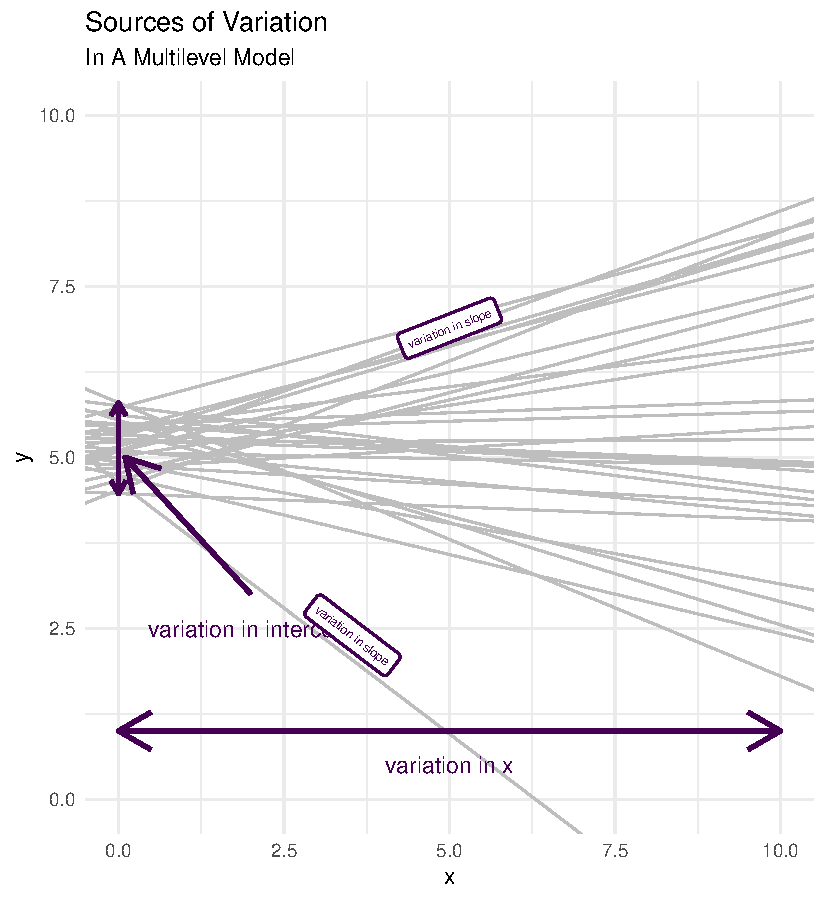
\includegraphics{cross-sectional_files/figure-pdf/fig-variationsources-1.pdf}

}

\caption{\label{fig-variationsources}Sources of Variation in a
Multilevel Model}

\end{figure}%

\subsection{Variation In Intercepts or
Outcomes}\label{variation-in-intercepts-or-outcomes}

In Equation~\ref{eq-MLMsubstantive2}, \(var(u_{0j})\) is the model
estimated amount of variation in the \emph{outcome}, \(y_{ij}\).

In the regression in Section~\ref{sec-regression}, there is discernible
between country variation, but more of the variation is between
individuals within the same country. Put another way, there is a
moderate tendency for children in families in the same country to have
similar outcomes, but two children in families in the same country may
also have very different outcomes. Children from families in different
countries may be as similar as children from families in the same
country.

\subsection{Variation In Predictors}\label{variation-in-predictors}

Equally important, I think, but much less frequently explored than
variation in \emph{outcomes}, is the possibility of variation in
\emph{predictors}, \(var(x_{ij})\). In the substantive example that we
have employed so far, the \emph{predictors} are different
\emph{parenting behaviors}, so considering variation in
\emph{predictors} allows us to consider variation in \emph{parenting
behaviors}, as well as variation in the \emph{outcomes} of those
behaviors.

We would estimate variation in behaviors attributable to country in much
the same way that we would estimate variation in outcomes, estimating an
unconditional model, but substituting \(x\) for \(y\).\footnote{Here for
  the sake of clarity, I use \(w_{0j}\) as a random effect to think
  about country specific variation in \(x\).}

\begin{equation}\phantomsection\label{eq-unconditionalx}{x_{ij} = \beta_0 + w_{0j} + e_{ij}}\end{equation}

Then, similarly, the variation in a predictor attributable to the
clustered nature of the data--in this case the clustering of individuals
in countries--is given by:

\begin{equation}\phantomsection\label{eq-ICCx}{\text{ICC}_x = \frac{var(w_{0j})}{var(w_{0j}) + var(e_{ij})}}\end{equation}

\subsection{Variation in Slopes}\label{variation-in-slopes}

Another possible type of variation to investigate is variation in the
relationship of \(x\) and \(y\), which is represented in the multilevel
model by examining variation in the \(\beta\)'s, i.e.~\(var(u_{1j})\).

\subsection{Summary}\label{summary}

Thus, we can consider a number of sources of possible variation.

\begin{longtable}[]{@{}
  >{\raggedright\arraybackslash}p{(\columnwidth - 2\tabcolsep) * \real{0.5750}}
  >{\raggedright\arraybackslash}p{(\columnwidth - 2\tabcolsep) * \real{0.4250}}@{}}
\caption{Some Possible Sources of Variation To Consider in A Multilevel
Model}\label{tbl-sourcesvariation}\tabularnewline
\toprule\noalign{}
\begin{minipage}[b]{\linewidth}\raggedright
Model Parameter
\end{minipage} & \begin{minipage}[b]{\linewidth}\raggedright
Meaning
\end{minipage} \\
\midrule\noalign{}
\endfirsthead
\toprule\noalign{}
\begin{minipage}[b]{\linewidth}\raggedright
Model Parameter
\end{minipage} & \begin{minipage}[b]{\linewidth}\raggedright
Meaning
\end{minipage} \\
\midrule\noalign{}
\endhead
\bottomrule\noalign{}
\endlastfoot
Independent Variables & \\
\(var(x_{ij})\) & What is the variation in x? \\
\(range(x_{ij})\) & What are the maximum and minimum of x? \\
\(var(w_{0j}) \text{ if } x = \beta_0 + w_{0j} + e_{ij}\) & What is the
country specific variation in the value of x? \\
Dependent Variable & \\
\(var(y_{ij})\) & What is the variation in y? \\
\(range(y_{ij})\) & What are the maximum and minimum of y? \\
\(var(u_{0j})\) & What is the country specific variation in the
intercept of y? \\
Regression Coefficients for Slopes & \\
\(\beta_{x} x\) & What is the relationship of x and y? \\
\(\beta_{xz} z \times x\) & What is the effect of z on the relationship
of x and y? \\
\(var(u_{1j}) \text{ from } u_{1j} \times x\) & What is the country
specific variation in the relationship of x and y? \\
\(cov(u_{0j}, u_{1j})\) & What is the covariance of the country specific
intercept and and country specific slope. Is the country specific
intercept related to the country specific slope? \\
\end{longtable}

\subsection{Variation As An Outcome}\label{variation-as-an-outcome}

Even less common is to examine \emph{variation} itself as an outcome
(Burkner, 2018).

\begin{equation}\phantomsection\label{eq-distributional}{\sigma_{yij} = \beta_0 + \beta_1 x_1 + u_{0j} + e_{ij}}\end{equation}

Here, the variation in the outcome, \(\sigma_{yij}\), rather than the
mean level of the outcome, \(y_{ij}\), is the focus of interest. My
notation for Equation~\ref{eq-distributional} draws upon Burkner
(2018)'s notation, but is modified in order to be consistent with the
rest of this document.

Why might such models be of conceptual interest? Imagine for example,
that the \emph{variation} in psychological well-being is higher in
countries with higher levels of poverty, or higher levels of income
inequality. The use of such models as this, discussed in more detail by
Burkner (2018), would allow us to explore such a question.

Of note, while I do not explore in detail differences between Bayesian
and frequentist approaches to multilevel modeling in this document,
these models are likely to be only estimable with Bayesian software
rather than with frequentist software (Burkner, 2018).

\subsection{Maximal Models}\label{maximal-models}

Hypothetically, one might imagine that there could be group level
unobserved factors which affect regression slopes: i.e.~the relationship
between a predictor x and outcome variable y. Arguably, were one to
ignore these unobserved factors in statistical estimation, they would
show up either in an error term, or in the regression coefficients
themselves. Were they to show up in the regression coefficients this
would represent statistical bias and a substantive mis-estimation of
important effects. thus, there is a conceptual argument for including as
many random effects---i.e.~random slopes---in a statistical model as
possible.

Models with all possible random effects are termed \emph{maximal models}
(Barr et al., 2013; Frank, 2018). Such models include a large number of
random slopes,
e.g.~\(u_1 \times x_1, u_2 \times x_2, u_3 \times x_3, ..., \text{etc.}\)
even when some of those estimated slopes are close to 0. Such models may
be more easily estimable when using Bayesian estimation (Frank, 2018), a
topic which I do not cover in detail in this document.

It should be noted that Matuschek et al. (2017) argue that such a
\emph{maximal} approach may lead to a loss of statistical power and
further argue that one should adhere to ``a random effect structure that
is supported by the data.'' In contrast, Nalborczyk et al. (2019) argue
that maximal models are supported under the Bayesian approach. Oberauer
(2022) also argues for including multiple random slopes. Schielzeth \&
Forstmeier (2009) make a similar argument from a frequentist
perspective.

\bookmarksetup{startatroot}

\chapter{The Longitudinal Multilevel
Model}\label{the-longitudinal-multilevel-model}

\begin{quote}
``Mathematics is the art of giving the same name to different things.''
(Poincare, 1908)
\end{quote}

Counter-intuitively, and surprisingly, the mathematics of estimating
models with cross-sectional clustered data easily generalizes to
longitudinal data. In cross sectional clustered data, we imagine
\emph{individuals or families clustered in neighborhoods, schools, or
countries}.

\begin{longtable}[]{@{}ll@{}}
\caption{Levels in Cross-Sectional
Data}\label{tbl-levelscrosssectional}\tabularnewline
\toprule\noalign{}
Level & Example(s) \\
\midrule\noalign{}
\endfirsthead
\toprule\noalign{}
Level & Example(s) \\
\midrule\noalign{}
\endhead
\bottomrule\noalign{}
\endlastfoot
1 & Individuals or Families \\
2 & Schools \\
& Neighborhoods \\
& Countries \\
\end{longtable}

In longitudinal data, we consider the \emph{first level} to be that of
\emph{time points}, or \emph{study waves}, which we sometimes call the
\emph{person-observation}.\footnote{When we are studying families,
  e.g.~a parent-child pair, it might be more appropriate to call each
  row of data a \emph{family-observation}, but the term
  \emph{person-observation} is more commonly used.} The \emph{second
level} is then the individual or family.

\begin{longtable}[]{@{}ll@{}}
\caption{Levels in Longitudinal
Data}\label{tbl-levelslongitudinal}\tabularnewline
\toprule\noalign{}
Level & Example(s) \\
\midrule\noalign{}
\endfirsthead
\toprule\noalign{}
Level & Example(s) \\
\midrule\noalign{}
\endhead
\bottomrule\noalign{}
\endlastfoot
1 & Timepoints \\
2 & Individuals or Families \\
\end{longtable}

While it is less common, we could then easily add additional clustering
to this longitudinal model, for example, clustering of individuals or
families inside social units.

\begin{longtable}[]{@{}ll@{}}
\caption{Multiple Levels in Longitudinal
Data}\label{tbl-levelslongitudinal2}\tabularnewline
\toprule\noalign{}
Level & Example(s) \\
\midrule\noalign{}
\endfirsthead
\toprule\noalign{}
Level & Example(s) \\
\midrule\noalign{}
\endhead
\bottomrule\noalign{}
\endlastfoot
1 & Timepoints \\
2 & Individuals or Families \\
3 & Schools \\
& Neighborhoods \\
& Countries \\
\end{longtable}

\section{Use Data With Multiple Observations Per
Individual}\label{use-data-with-multiple-observations-per-individual}

Multilevel data suitable for longitudinal analysis has \emph{multiple
rows of data per individual or family}. Put another way, \emph{every row
of data is a person-timepoint}.

\begin{quote}
This method of organizing data is known as the \emph{long} format.
Another way of organizing longitudinal data--which I do not discuss in
detail here--is the \emph{wide} format in which every individual or
family has only a single row of data. In \emph{wide} data, the different
timepoints are in \emph{different columns} of data. I do discuss
\emph{reshaping} data from \emph{wide} to \emph{long}, and vice versa,
in Appendix~\ref{sec-reshape}.
\end{quote}

\begin{longtable}[]{@{}lll@{}}
\caption{Data in Long Format}\label{tbl-datalong}\tabularnewline
\toprule\noalign{}
id & t & x \\
\midrule\noalign{}
\endfirsthead
\toprule\noalign{}
id & t & x \\
\midrule\noalign{}
\endhead
\bottomrule\noalign{}
\endlastfoot
1 & 1 & 10 \\
1 & 2 & 20 \\
1 & 3 & 30 \\
2 & 1 & 20 \\
2 & 2 & 30 \\
2 & 3 & 40 \\
\end{longtable}

\begin{longtable}[]{@{}llll@{}}
\caption{Data in Wide Format}\label{tbl-datawide}\tabularnewline
\toprule\noalign{}
id & x1 & x2 & x3 \\
\midrule\noalign{}
\endfirsthead
\toprule\noalign{}
id & x1 & x2 & x3 \\
\midrule\noalign{}
\endhead
\bottomrule\noalign{}
\endlastfoot
1 & 10 & 20 & 30 \\
2 & 20 & 30 & 40 \\
\end{longtable}

\section{Simulated Multilevel Longitudinal
Data}\label{simulated-multilevel-longitudinal-data}

For the discussion below, I use a longitudinal version of the simulated
data that has multiple rows of data per family.

\begin{longtable}[]{@{}
  >{\centering\arraybackslash}p{(\columnwidth - 16\tabcolsep) * \real{0.1190}}
  >{\centering\arraybackslash}p{(\columnwidth - 16\tabcolsep) * \real{0.0714}}
  >{\centering\arraybackslash}p{(\columnwidth - 16\tabcolsep) * \real{0.1071}}
  >{\centering\arraybackslash}p{(\columnwidth - 16\tabcolsep) * \real{0.0714}}
  >{\centering\arraybackslash}p{(\columnwidth - 16\tabcolsep) * \real{0.0952}}
  >{\centering\arraybackslash}p{(\columnwidth - 16\tabcolsep) * \real{0.0476}}
  >{\centering\arraybackslash}p{(\columnwidth - 16\tabcolsep) * \real{0.2619}}
  >{\centering\arraybackslash}p{(\columnwidth - 16\tabcolsep) * \real{0.1071}}
  >{\centering\arraybackslash}p{(\columnwidth - 16\tabcolsep) * \real{0.1190}}@{}}

\caption{\label{tbl-simulatedlongitudinaldata}Simulated Longitudinal
Multilevel Data}

\tabularnewline

\toprule\noalign{}
\begin{minipage}[b]{\linewidth}\centering
country
\end{minipage} & \begin{minipage}[b]{\linewidth}\centering
HDI
\end{minipage} & \begin{minipage}[b]{\linewidth}\centering
family
\end{minipage} & \begin{minipage}[b]{\linewidth}\centering
id
\end{minipage} & \begin{minipage}[b]{\linewidth}\centering
group
\end{minipage} & \begin{minipage}[b]{\linewidth}\centering
t
\end{minipage} & \begin{minipage}[b]{\linewidth}\centering
physical\_punishment
\end{minipage} & \begin{minipage}[b]{\linewidth}\centering
warmth
\end{minipage} & \begin{minipage}[b]{\linewidth}\centering
outcome
\end{minipage} \\
\midrule\noalign{}
\endhead
\bottomrule\noalign{}
\endlastfoot
1 & 69 & 1 & 1.1 & 2 & 1 & 2 & 3 & 59.18 \\
1 & 69 & 1 & 1.1 & 2 & 2 & 2 & 2 & 58.29 \\
1 & 69 & 1 & 1.1 & 2 & 3 & 3 & 3 & 60.58 \\
1 & 69 & 2 & 1.2 & 2 & 1 & 4 & 0 & 61.54 \\
1 & 69 & 2 & 1.2 & 2 & 2 & 4 & 0 & 55.96 \\
1 & 69 & 2 & 1.2 & 2 & 3 & 4 & 2 & 56.19 \\

\end{longtable}

Since I will be discussing the estimation of a \emph{longitudinal}
model, it is often useful to graph the outcome variable against time.

\begin{figure}

\centering{

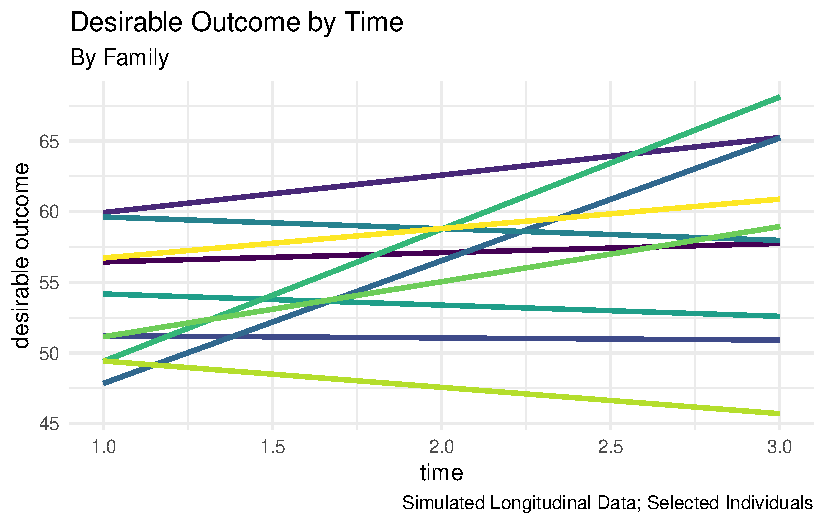
\includegraphics{longitudinal_files/figure-pdf/fig-data2-1.pdf}

}

\caption{\label{fig-data2}Graph of Simulated Longitudinal Data}

\end{figure}%

\section{The Equation}\label{the-equation-1}

When data are in \emph{long} format, the following equation is
applicable. Observe that the model below is a \emph{three level} model
where \emph{timepoints} are nested inside \emph{families} which in turn
are nested inside \emph{countries}. A simpler two level model with
\emph{timepoints} nested inside \emph{families} would also be possible
to estimate.

\begin{equation}\phantomsection\label{eq-MLM-longitudinal}{\text{outcome}_{itj} = \beta_0 + \beta_1 \text{parental warmth}_{itj} + \beta_2 \text{physical punishment}_{itj} + \beta_3 \text{time}_{itj} \ + }\end{equation}

\[\beta_4 \text{group}_{itj} + \beta_5 \text{HDI}_{itj} +\]

\[u_{0j} + u_{1j} \times \text{parental warmth}_{itj} \ + \]

\[v_{0i} + v_{1i} \times t_{itj} + e_{itj}\] Here I include a random
slope (\(u_{1j}\)) at the country level for parental warmth, as well as
a random slope (\(v_{1i}\)) at the family level for time.

As before, the random slope for parental warmth,
\(u_{1j} \times \text{parental warmth}_{ij}\) suggests allows us to
estimate whether the relationship between parental warmth and the
outcome varies across countries. The random slope for time,
\(v_{1i} \times t\), allows us to estimate whether time trajectories
(the slope for time) vary across families.

\section{Growth Trajectories}\label{growth-trajectories}

In longitudinal multilevel models, the variable for \emph{time} assumes
a special role as we are often visualizing a \emph{growth trajectory}
over the course of time.

Imagine a model as follows where \emph{group} is a (1/0) variable for
membership in one of two groups:

\[\text{outcome} = \beta_0 + \beta_t \text{time} + \beta_\text{group} \text{group} + \beta_\text{interaction} \text{group} \times \text{time} + u_{0i} + e_{it}\]
Then, each group has it's own intercept and time trajectory:

\begin{longtable}[]{@{}
  >{\raggedright\arraybackslash}p{(\columnwidth - 4\tabcolsep) * \real{0.1400}}
  >{\raggedright\arraybackslash}p{(\columnwidth - 4\tabcolsep) * \real{0.3000}}
  >{\raggedright\arraybackslash}p{(\columnwidth - 4\tabcolsep) * \real{0.5600}}@{}}
\caption{Slope and Intercept for Each
Group}\label{tbl-trajectory}\tabularnewline
\toprule\noalign{}
\begin{minipage}[b]{\linewidth}\raggedright
Group
\end{minipage} & \begin{minipage}[b]{\linewidth}\raggedright
Intercept
\end{minipage} & \begin{minipage}[b]{\linewidth}\raggedright
Slope (Time Trajectory)
\end{minipage} \\
\midrule\noalign{}
\endfirsthead
\toprule\noalign{}
\begin{minipage}[b]{\linewidth}\raggedright
Group
\end{minipage} & \begin{minipage}[b]{\linewidth}\raggedright
Intercept
\end{minipage} & \begin{minipage}[b]{\linewidth}\raggedright
Slope (Time Trajectory)
\end{minipage} \\
\midrule\noalign{}
\endhead
\bottomrule\noalign{}
\endlastfoot
0 & \(\beta_0\) & \(\beta_t\) \\
1 & \(\beta_0 + \beta_\text{group}\) &
\(\beta_t + \beta_\text{interaction}\) \\
\end{longtable}

\begin{quote}
Thus, in longitudinal multilevel models, \emph{main effects} modify the
\emph{intercept} of the time trajectory, while \emph{interactions with
time}, modify the \emph{slope} of the time trajectory.
\end{quote}

\begin{figure}

\centering{

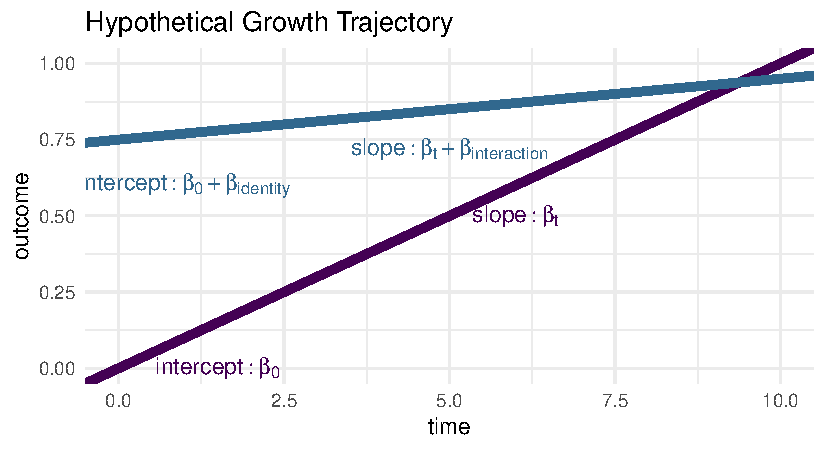
\includegraphics{longitudinal_files/figure-pdf/fig-trajectory-1.pdf}

}

\caption{\label{fig-trajectory}Hypothetical Growth Trajectory}

\end{figure}%

\section{Regression With Simulated Multi-Country Longitudinal
Data}\label{sec-regressionlongitudinal}

The Stata command that we use to analyze this data is:

\begin{Shaded}
\begin{Highlighting}[]

\NormalTok{mixed outcome t warmth physical\_punishment }\FunctionTok{group}\NormalTok{ HDI || country: warmth || id: t}
\end{Highlighting}
\end{Shaded}

\begin{longtable}[]{@{}lll@{}}
\toprule\noalign{}
& longitudinal & \\
\midrule\noalign{}
\endhead
\bottomrule\noalign{}
\endlastfoot
t & 0.988 & ** \\
warmth & 0.946 & ** \\
physical\_punishment & -0.927 & ** \\
group & & \\
2 & 0.986 & ** \\
HDI & 0.008 & \\
\_cons & 50.480 & ** \\
var(warmth) & 0.000 & \\
var(\_cons) & 3.651 & \\
var(\_cons) & 8.853 & \\
var(t) & 0.000 & \\
var(e) & 26.001 & \\
\end{longtable}

** p\textless.01, * p\textless.05

Examining the regression results, the results of the model suggest that
child outcomes improve over time. Better child outcomes are again
associated with parental \texttt{warmth}, and parental use of
\texttt{physical\_punishment} is associated with reduced child outcomes.
\texttt{HDI} is again not associated with outcomes.

\section{Autocorrelation}\label{autocorrelation}

When data are ordered by a time variable \(t\), it is possible that
observations that are closer together in time will have a higher
correlation than observations that are distant in time. In the simplest
example, \(e_{i, t=k}\) may be correlated with \(e_{i, t=k-1}\). This
phenomenon is known as \emph{autocorrelation}. As Hooper (2022) would
suggest, it may make sense to assume that the correlation between
observations ``decays with increasing separation in time''.

Most software programs for multilevel modeling allow one to incorporate
measures of autocorrelation so that, e.g., \(e_{i,t=3}\) is allowed to
be correlated with \(e_{i,t=2}\), which in turn can be correlated with
\(e_{i,t=1}\). More complex autocorrelation structures are usually also
possible (StataCorp, 2021a).

\section{Causality}\label{causality}

\subsection{The Importance of Causal
Reasoning}\label{the-importance-of-causal-reasoning}

Causal reasoning is sometimes considered to be a statistical--or even
overly technical--concern. Arguably, however, whenever one is using
research to make recommendations about \emph{interventions}, or
\emph{treatments}, or \emph{policies}, one is engaging in some form of
causal reasoning (Duncan \& Gibson-Davis, 2006).

\begin{quote}
If one is saying that implementing \emph{x} would result in beneficial
changes in \emph{y}, one is arguing--at least implicitly--that \emph{x}
is one of the causes of \emph{y}.
\end{quote}

It then behooves one to be explicit about this chain of causal
reasoning. For example, to continue one of the substantive examples of
this document, if one is going to argue for programs, interventions, or
treatments that promote \emph{parental warmth}, or that discourage
parental use of \emph{physical punishment} with the aim of improving
children's \emph{mental health}, one must be at least reasonably sure
that \emph{parental warmth} and \emph{physical punishment} are
\emph{causes} of children's mental health.

In a statement salient for social research, Duncan \& Gibson-Davis
(2006) point out the logical inconsistency of writing that does not
rigorously address causal processes, but then goes on to suggest
interventions or treatment or policies:

\begin{quote}
``Developmental studies are usually careful to point out when their data
do not come from a randomized experiment. As with much of the
nonexperimental literature in developmental psychology, most of the
articles then go on to assert that, as a consequence, it is impossible
to draw causal inferences from the analysis. Indeed, much of their
language describing results is couched in terms of `associations'
between child care quality and child outcomes. It is not uncommon,
however, to see these papers make explicit statements about effects, and
others draw explicit policy conclusions. For instance, NICHD (1997, 876)
stated, `The interaction analyses provided evidence that high-quality
child care served a compensatory function for children whose maternal
care was lacking.' On the policy side, NICHD (2002c, 199) asserted,
`These findings provide empirical support for policies that improve
state regulations for caregiver training and child-staff ratios.'\,''
\end{quote}

\begin{quote}
``One cannot have it both ways. Studies that do not aspire to causal
analysis should make no claim whatsoever about effects and draw no
policy conclusions. At the same time, it would be a terrible waste of
resources to conduct expensive longitudinal studies without attempting
to use them for causal modeling.''
\end{quote}

\subsection{Randomized Controlled
Trials}\label{randomized-controlled-trials}

Randomized studies provide the best evidence about \emph{internal
validity} and causal relationships. However, randomized studies have
certain important limitations (Diener et al., 2022). First of
all--especially in a study with a smaller sample--randomization may not
always be perfect, and the control and treatment groups may not be
statistically equivalent. Secondly, because randomized studies are
costly to conduct, they may have small samples and may be statistically
underpowered. Smaller samples and underpowered studies are more likely
to generate false positive results than larger samples (Button et al.,
2013) \footnote{See
  \url{https://agrogan.shinyapps.io/Thinking-Through-Bayes/} for a
  demonstration of this idea from a Bayesian perspective.}. Further, and
importantly, because of ethical concerns some studies can not be
conducted with randomization (Diener et al., 2022). For example, in the
study of parenting and child development, children cannot ethically be
assigned to parents with different styles of parenting and followed over
the long term (Heilmann et al., 2021). Finally, and crucially, because
of their often small samples, and their often rigorous exclusion
criteria, randomized studies may have high internal validity, but much
lower external validity, or generalization to larger populations (Diener
et al., 2022). This issue of generalizability becomes increasingly
salient, when we are reminded of the fact that so little social and
psychological research has been conducted outside of North American
contexts (Draper et al., 2022; Henrich et al., 2010). Thus, methods that
provide rigorous causal estimation with observational methods are
necessary (Diener et al., 2022).

\subsection{Observational Studies and
Causality}\label{observational-studies-and-causality}

Because of the assumed superiority of studies that employ randomization,
it is sometimes maintained that \emph{correlation is not causation} and
that studies that do not make use of randomization are \emph{only
observational} and \emph{correlational}, and that results from
observational studies cannot be used to support causal conclusions.
However, in an important review (Waddington et al., 2022) suggested that
studies using appropriately quantitative methods can provide causally
robust conclusions. Heilmann et al. (2021) make a similar assertion with
specific regard to studies of physical punishment and child outcomes,
arguing that observational studies that make use of appropriately
advanced quantitative methods can make causally robust conclusions about
the effects of physical discipline.

It is necessary to make use of broadly representative observational data
sets, and appropriately sophisticated quantitative methods, to make
causally robust conclusions from observational data that are applicable
across diverse populations.

\subsection{Formal Criteria of
Causality}\label{formal-criteria-of-causality}

For x to be a cause of y, one needs the following 3 things to be true
(Holland, 1986).

\begin{enumerate}
\def\labelenumi{\arabic{enumi}.}
\tightlist
\item
  \emph{x} is (are) associated with (correlated with) \emph{y}.
\item
  \emph{x} come(s) before \emph{y} in time.
\item
  \emph{z}--or other factors--cannot explain the association of
  (correlation of) \emph{x} and \emph{y}.
\end{enumerate}

\begin{figure}

\centering{

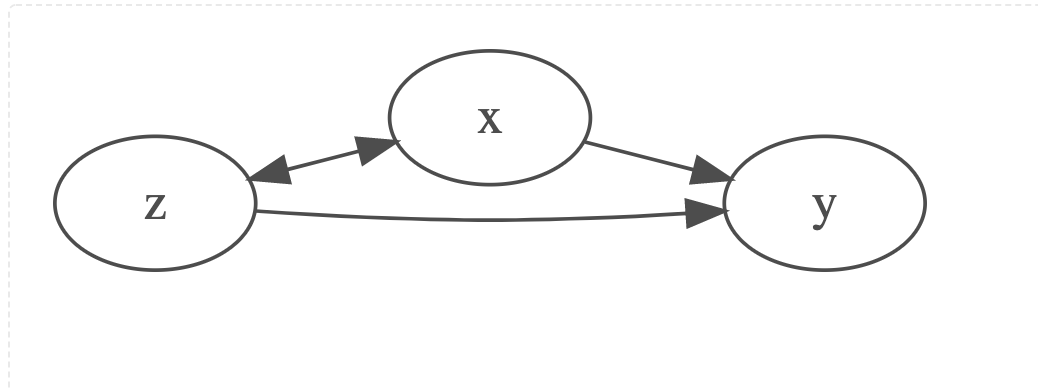
\includegraphics[width=3.46in,height=\textheight]{fig-causality.png}

}

\caption{\label{fig-causality}Formal Criteria of Causality}

\end{figure}%

\begin{quote}
If \emph{z} is omitted from the regression model, then the estimates for
\(x \rightarrow y\) (i.e.~\(\beta_{x \rightarrow y}\)) will be biased.
In a common scenario, \(\beta_{x \rightarrow y}\) may be an
over-estimate of the effect, and statistical significance of
\(\beta_{x \rightarrow y}\) may represent a false positive.
\end{quote}

It is likely useful to restate the above abstract statements in terms of
the substantive issues that I have been considering so far in this
document.

For \emph{parenting} to be a cause of \emph{child outcomes}, one needs
the following 3 things to be true (Holland, 1986).

\begin{enumerate}
\def\labelenumi{\arabic{enumi}.}
\tightlist
\item
  \emph{parenting} is (are) associated with (correlated with)
  \emph{child outcomes}.
\item
  \emph{parenting} come(s) before \emph{child outcomes} in time.
\item
  \emph{SES}, \emph{community characteristics}--or other factors--cannot
  explain the association of (correlation of) \emph{parenting} and
  \emph{child outcomes}.
\end{enumerate}

\begin{figure}

\centering{

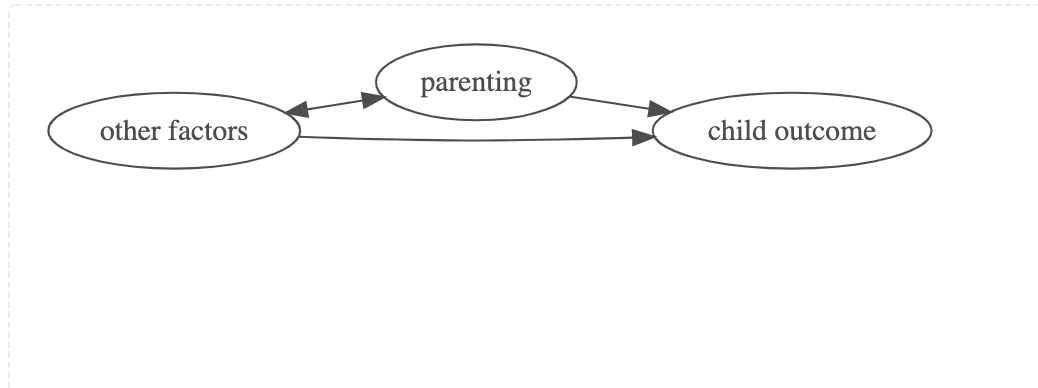
\includegraphics[width=3.46in,height=\textheight]{fig-causalitysubstantive.png}

}

\caption{\label{fig-causalitysubstantive}Formal Criteria of Causality: A
Substantive Example}

\end{figure}%

If \emph{other factors} are omitted from the regression model, then the
estimates for \(\text{parenting} \rightarrow \text{child outcome}\)
(i.e.~\(\beta_{\text{parenting} \rightarrow \text{child outcome}}\))
will be biased. In a common scenario,
\(\beta_{\text{parenting} \rightarrow \text{child outcome}}\) may be an
over-estimate of the effect, and statistical significance of
\(\beta_{\text{parenting} \rightarrow \text{child outcome}}\) may
represent a false positive.

\subsection{Simpson's Paradox}\label{simpsons-paradox}

Earlier, in Section~\ref{sec-multilevelstructure}, I referred to the
idea of \emph{multilevel structure} wherein failure to account for the
clustering of data--omission of \(u_0\) from the equation being
estimated--may lead to incorrect conclusions. A closely related
phenomenon is that of \emph{Simpson's Paradox} (Simpson, 1951) wherein
omission of a relevant \emph{covariate} (e.g.~\(z_{it}\) such as SES,
community characteristics, country level characteristics) may also lead
to dramatically incorrect results.

Statistically, we imagine a situation where the true model is:

\[\text{child outcome}_{it} = \beta_0 + \beta_1 \text{parenting}_{it} +\]

\[\beta_2 \text{individual or family or community or country characteristic}_{it} + \]
\[u_{0i} + e_{it}\]

If \emph{individual or family or community or country characteristics}
in fact influence \emph{outcome}, but are not included in the
statistical model, perhaps because they are not measured in the data,
then the estimate of \(\beta_1\) for \emph{parenting} will be biased.
See Figure~\ref{fig-Simpson} for an illustration. When possible
confounders are \emph{measured}, we can include those variables in the
statistical model. When possible confounders are \emph{unmeasured}, we
need to try to use methods that capture those \emph{unmeasured}
confounders.

\begin{figure}

\centering{

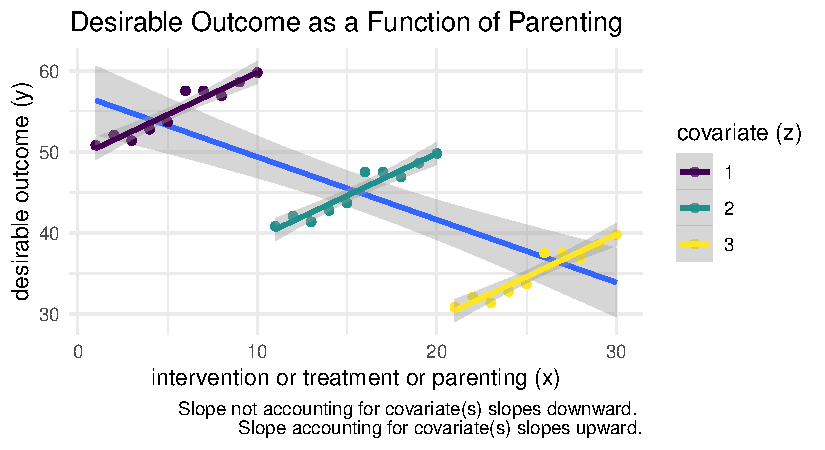
\includegraphics{longitudinal_files/figure-pdf/fig-Simpson-1.pdf}

}

\caption{\label{fig-Simpson}An Illustration of Simpson's Paradox}

\end{figure}%

\subsection{A Simpler Multilevel Model To Explore
Causality}\label{a-simpler-multilevel-model-to-explore-causality}

For purposes of explication of ideas about causal estimation, in this
section, I imagine a simpler equation where I am only considering the
clustering of \emph{person timepoints} within \emph{individual people},
and ignoring for the moment--again for the sake of exposition--the
clustering of \emph{individuals} within \emph{countries}.

After explication and comprehension of this model, however, it is a
simple matter to add back in the random effects for country level
clustering.

The appropriate multilevel model is below.

\begin{equation}\phantomsection\label{eq-MLM-simpler}{\text{outcome}_{it} = \beta_0 + \beta_1 \text{parental warmth}_{it} + \beta_2 \text{physical punishment}_{it} + \beta_3 \text{time}_{it} \ + }\end{equation}

\[\beta_4 \text{group}_{it} + \beta_5 \text{HDI}_{it} \ +\]

\[v_{0i} + e_{it}\]

Note that in Equation~\ref{eq-MLM-simpler}, if one were estimating a
\emph{multilevel model}, one would consider the \(v_{0i}\) to be a
randomly varying parameter with a mean of 0, and a variance of
\(\sigma^2(v_{0i})\).

\subsection{Fixed Effects Regression}\label{fixed-effects-regression}

I can use the same equation:

\begin{equation}\phantomsection\label{eq-FE}{\text{outcome}_{it} = \beta_0 + \beta_1 \text{parental warmth}_{it} + \beta_2 \text{physical punishment}_{it} + \beta_3 \text{time}_{it} \ + }\end{equation}

\[\beta_4 \text{group}_{it} + \beta_5 \text{HDI}_{it} \ +\]

\[v_{0i} + e_{it}\]

However, in Equation~\ref{eq-FE}, I now consider the \(v_{0i}\) to be
\emph{estimable} for each individual \(i\) in the data. In effect, the
\(v_{0i}\) become a unique indicator variable for each individual in the
data set. This is known as a \emph{fixed effects regression model}.

Recall the discussion in Section~\ref{sec-withinbetween}. In essence, in
the fixed effects regression model, I am only making use of the
variation within individuals, and not making use of the variation
between individuals.

Details are provided in Allison (2009) and Wooldridge (2010). StataCorp
(2021c) provides an exceptionally clear explication of the core idea of
fixed effects regression. The essential idea is that the fixed effects
model provides statistical control for all time invariant
characteristics of study participants, such as--as is often the case in
many data sets--their racial or ethnic identity, their neighborhood of
residence, or other characteristics which by definition are time
invariant, such as the region of the country or city in which a
respondent was born. Importantly, (Ma et al., 2018) note that:

\begin{quote}
``Another potential omitted variable is that of genetic predisposition,
in that observed neighborhood effects on child outcomes are possibly
attributable to a genetic heritage shared by parents and their child
(Caspi et al., 2000).''
\end{quote}

Such genetic heritage could be considered to be a time invariant
variable that, while unobserved, would be controlled for by a fixed
effects regression.

Thus, by ruling out many potential confounds, fixed effects regression
methods provide much more causally robust analyses, specifically because
they control for many more possible confounding variables than do
standard regression methods, including multilevel models, which are only
able to control for the variables that are measured in the study
\emph{and} that are included within the regression model.

However, a disadvantage of the fixed effects approach is that this
approach can not provide estimates for any time invariant characteristic
of study participants. Indeed, if one includes time invariant variables
into a fixed effects regression, they are automatically dropped from the
regression results as can be seen in the regression table below.

The relevant Stata commands are:

\begin{itemize}
\tightlist
\item
  Multilevel Model:
  \texttt{mixed\ outcome\ t\ warmth\ physical\_punishment\ group\ HDI\ \textbar{}\textbar{}\ id:}
\item
  Fixed Effects Model:
  \texttt{xtreg\ outcome\ t\ warmth\ physical\_punishment\ group\ HDI,\ i(id)\ fe}
\end{itemize}

\begin{longtable}[]{@{}lllll@{}}
\toprule\noalign{}
& MLM & & FE & \\
\midrule\noalign{}
\endhead
\bottomrule\noalign{}
\endlastfoot
t & 0.988 & ** & 0.988 & ** \\
warmth & 0.947 & ** & 0.970 & ** \\
physical\_punishment & -0.910 & ** & -1.033 & ** \\
group & & & & \\
2 & 0.997 & ** & & \\
HDI & 0.008 & & & \\
\_cons & 50.429 & ** & 51.640 & ** \\
var(\_cons) & 12.497 & & & \\
var(e) & 26.003 & & & \\
Number of observations & & & 9000 & \\
\end{longtable}

** p\textless.01, * p\textless.05

In comparing the multilevel model and the fixed effects regression, we
note a few salient difference. First, the fixed effects are similar to
the multilevel model coefficients. (Most often, the fixed effect
regression coefficients are attenuated versions of the multilevel model
coefficients, but not always.) The fixed effects regression coefficients
for variables that have some variation over time, provide estimates that
control for all time invariant variables in the model.

Second, estimates for any quantities that do not vary over time, in this
case, \texttt{group} membership, and \texttt{HDI}, are not available
from the fixed effects regression.

\subsection{The Correlated Random Effects
Model}\label{the-correlated-random-effects-model}

The \emph{correlated random effects} model is based upon ideas first
developed by Mundlak (1978) and later explicated in Wooldridge (2010).
Antonakis et al. (2021) and Schunck (2013) provide very intuitive
explanations of this model.

The central idea is that one can obtain estimates of both the time
invariant variables, and estimates for time varying variables. The key
idea is that for time varying variables, I include the \emph{individual}
level mean for that variable in the model. Thus, in the example below, I
include \(\beta_{1a}\overline{\text{parental warmth}}_{i}\) and
\(\beta_{2a}\overline{\text{physical punishment}}_{i}\). \footnote{The
  correlated random effects model can also be applied cross-sectionally,
  but the model is much easier to explicate in the longitudinal context.}
This is similar in approach to what is described in
Section~\ref{sec-withinbetween}, however, here I am simply adding the
group level mean to the equation instead of decomposing independent
variables into within and between components.

\begin{equation}\phantomsection\label{eq-CRE}{\text{outcome}_{it} = \beta_0 + \beta_1 \text{parental warmth}_{it} + \beta_{1a}\overline{\text{parental warmth}}_{i} \ + }\end{equation}

\[\beta_2 \text{physical punishment}_{it} + \beta_{2a}\overline{\text{physical punishment}}_{i} + \]

\[\beta_3 \text{time}_{it} \ + \]

\[\beta_4 \text{group}_{it} + \beta_5 \text{HDI}_{it} \ +\]

\[v_{0i} + e_{ij}\]

By including these parameters, I obtain estimates for the time varying
variables that are \emph{equivalent} to what I would obtain from a fixed
effects regression (Schunck, 2013).

The Stata command for the correlated random effects model is:

\begin{Shaded}
\begin{Highlighting}[]

\NormalTok{mixed outcome t warmth mean\_warmth physical\_punishment mean\_physicalpunishment }\FunctionTok{group}\NormalTok{ HDI || id:}
  
\end{Highlighting}
\end{Shaded}

\begin{longtable}[]{@{}lllllll@{}}
\toprule\noalign{}
& MLM & & FE & & CRE & \\
\midrule\noalign{}
\endhead
\bottomrule\noalign{}
\endlastfoot
t & 0.988 & ** & 0.988 & ** & 0.988 & ** \\
warmth & 0.947 & ** & 0.970 & ** & 0.970 & ** \\
physical\_punishment & -0.910 & ** & -1.033 & ** & -1.033 & ** \\
group & & & & & & \\
2 & 0.997 & ** & & & 0.995 & ** \\
HDI & 0.008 & & & & 0.008 & \\
mean\_warmth & & & & & -0.032 & \\
mean\_physicalpunishment & & & & & 0.214 & * \\
\_cons & 50.429 & ** & 51.640 & ** & 50.224 & ** \\
var(\_cons) & 12.497 & & & & & \\
var(e) & 26.003 & & & & 25.993 & \\
var(\_cons) & & & & & 12.488 & \\
Number of observations & & & 9000 & & & \\
\end{longtable}

** p\textless.01, * p\textless.05

Note a couple of things from this table. First, results from the
correlated random effects model, and the fixed effects regression model
are exactly the same for \emph{time varying} variables, \texttt{t},
\texttt{warmth}, and \texttt{physical\_punishment}. Again, these
coefficients for \emph{time varying} variables are estimated with
statistical control for all time invariant characteristics of study
subjects, whether those characteristics are observed, or unobserved.
Secondly, unlike the fixed effects regression, coefficients for
\emph{time invariant} variables, e.g.~\texttt{group}, \texttt{HDI}, mean
levels of \texttt{warmth}, and mean levels of
\texttt{physical\_punishment} are provided, while they are not provided
in the fixed effects model.

\bookmarksetup{startatroot}

\chapter{Conclusion}\label{conclusion}

\begin{quote}
``We have peered into a new world and have seen that it is more
mysterious and more complex than we had imagined.'' (Rubin, 1997)
\end{quote}

\begin{quote}
``To take on a new perspective obviously does not mean throwing out all
of our knowledge; what it supposes, rather, is that we will relativize
that knowledge and critically revise it from the perspective of the
popular majorities. Only then will the theories and models show their
validity or deficiency, their utility or lack thereof, the universality
or provincialism. Only then will the techniques we have learned display
their liberating potential or their seeds of subjugation.''
(Martin-Baro, 1994b)
\end{quote}

Many data sets relevant to the study of important social issues, or
social problems, are inherently multilevel. For example, data on diverse
children in schools, diverse individuals in neighborhoods, and
individuals or families in diverse and different countries all have
multilevel structures in which individuals are clustered in higher level
social structures. Data with repeated measures, sometimes termed panel
data, can also be thought of as multilevel data sets, wherein individual
timepoints are nested inside individuals, who may in turn be nested or
clustered in larger social units such as countries.

Failure to use appropriate basic multilevel models with such multilevel
data can lead to answers that are either biased, or demonstrably wrong.
Simple multilevel models allow the researcher to correctly estimate
statistical significance, and to correctly estimate regression
coefficients while accounting for multilevel structure. More advanced
applications of multilevel models allow the researcher to explore the
variation in both predictors and outcomes--and the relationship of
predictors to outcomes--and to characterize the extent of this
variation. Lastly, multilevel models provide a foundation for thinking
about closely related models--fixed effects regression, and correlated
random effects models--that provide methods for estimation that afford
stronger causal conclusions.

Thus, for applied researchers, interested in addressing a variety of
social problems and social issues with diverse samples of individuals,
multilevel models present a method to think clearly about variation, to
explore that variation, and to extend that thinking about variation to
estimate more causally robust models within the context of diversity and
variation.

\bookmarksetup{startatroot}

\chapter*{References}\label{references}
\addcontentsline{toc}{chapter}{References}

\markboth{References}{References}

\phantomsection\label{refs}
\begin{CSLReferences}{1}{0}
\bibitem[\citeproctext]{ref-Abelson1995}
Abelson, R. P. (1995). Statistics as principled argument. In
\emph{Statistics as principled argument.} (pp. 221, xv, 221--xv).
Lawrence Erlbaum Associates, Inc.

\bibitem[\citeproctext]{ref-Allison2009}
Allison, P. (2009). \emph{Fixed effects regression models}. Sage
Publishing.

\bibitem[\citeproctext]{ref-Antonakis2019}
Antonakis, J., Bastardoz, N., \& Ronko, M. (2021). On ignoring the
random effects assumption in multilevel models: Review, critique, and
recommendations. \emph{Organizational Research Methods}, \emph{24},
443--483. \url{https://doi.org/10.1177/1094428119877457}

\bibitem[\citeproctext]{ref-Aron1994}
Aron, A., \& Corne, S. (1994). Introduction. In A. Aron \& S. Corne
(Eds.), \emph{Writings for a liberation psychology}. Harvard University
Press.

\bibitem[\citeproctext]{ref-Barr2013}
Barr, D. J., Levy, R., Scheepers, C., \& Tily, H. J. (2013). Random
effects structure for confirmatory hypothesis testing: Keep it maximal.
\emph{Journal of Memory and Language}, \emph{68}(3), 255--278.
\url{https://doi.org/10.1016/j.jml.2012.11.001}

\bibitem[\citeproctext]{ref-Barth2020}
Barth, R. P., \& Olsen, A. N. (2020). Are children oppressed? The timely
importance of answering this question. \emph{Children and Youth Services
Review}, \emph{110}, 104780.
\url{https://doi.org/10.1016/j.childyouth.2020.104780}

\bibitem[\citeproctext]{ref-Bland1994}
Bland, J. M., \& Altman, D. G. (1994). Statistics notes: Correlation,
regression, and repeated data. \emph{BMJ}, \emph{308}, 896.
\url{https://doi.org/10.1136/bmj.308.6933.896}

\bibitem[\citeproctext]{ref-Blasi2022}
Blasi, D. E., Henrich, J., Adamou, E., Kemmerer, D., \& Majid, A.
(2022). Over-reliance on {E}nglish hinders cognitive science.
\emph{Trends in Cognitive Sciences}.
\url{https://doi.org/10.1016/j.tics.2022.09.015}

\bibitem[\citeproctext]{ref-Burkner2018}
Burkner, P.-C. (2018). Advanced {B}ayesian multilevel modeling with the
{R} package brms. \emph{The R Journal}, \emph{10}(1), 395--411.

\bibitem[\citeproctext]{ref-Burton2005}
Burton, M., \& Kagan, C. (2005). {Liberation Social Psychology: Learning
From Latin America Psychology of liberation: Learning from Latin
America}. \emph{Journal of Community \& Applied Social Psychology},
\emph{15}. \url{https://doi.org/10.1002/casp.786}

\bibitem[\citeproctext]{ref-Button2013}
Button, K. S., Ioannidis, J. P. A., Mokrysz, C., Nosek, B. A., Flint,
J., Robinson, E. S. J., \& Munaf`o, M. R. (2013). Power failure: Why
small sample size undermines the reliability of neuroscience.
\emph{Nature Reviews Neuroscience}, \emph{14}, 365--376.
\url{https://doi.org/10.1038/nrn3475}

\bibitem[\citeproctext]{ref-Caspi2000}
Caspi, A., Taylor, A., Moffitt, T. E., \& Plomin, R. (2000).
Neighborhood deprivation affects children's mental health: Environmental
risks identified in a genetic design. \emph{Psychological Science},
\emph{11}(4), 338--342. \url{https://doi.org/10.1111/1467-9280.00267}

\bibitem[\citeproctext]{ref-Cesaire1956}
Cesaire, A. (1956). \emph{Letter to {M}aurice {T}horez}.

\bibitem[\citeproctext]{ref-Cokley2013}
Cokley, K., \& Awad, G. (2013). In defense of quantitative methods:
Using the {``master's tools''} to promote social justice. \emph{Journal
for Social Action in Counseling \& Psychology}, \emph{5}, 26.
\url{https://doi.org/10.33043/JSACP.5.2.26-41}

\bibitem[\citeproctext]{ref-Dalton2000}
Dalton, R. (2000). Como t{ú}. In M. Espada (Ed.), \emph{Poetry like
bread: Poets of the political imagination}. Curbstone Press.

\bibitem[\citeproctext]{ref-Deater-Deckard1996}
Deater-Deckard, K., Dodge, K. A., Bates, J. E., \& Pettit, G. S. (1996).
{Physical discipline among African American and European American
mothers: Links to children's externalizing behaviors.}
\emph{Developmental Psychology}, \emph{32}(6), 1065--1072.
\url{https://doi.org/10.1037/0012-1649.32.6.1065}

\bibitem[\citeproctext]{ref-Diener2022}
Diener, E., Northcott, R., Zyphur, M. J., \& West, S. G. (2022). Beyond
experiments. \emph{Perspectives on Psychological Science}, \emph{17},
1101--1119. \url{https://doi.org/10.1177/17456916211037670}

\bibitem[\citeproctext]{ref-Dove1999}
Dove, R. (1999). The first book. In \emph{On the bus with {R}osa
{P}arks}. W.W. Norton.

\bibitem[\citeproctext]{ref-Draper2022}
Draper, C. E., Barnett, L. M., Cook, C. J., Cuartas, J. A., Howard, S.
J., McCoy, D. C., Merkley, R., Molano, A., Maldonado-Carreño, C.,
Obradovic, J., Scerif, G., Valentini, N. C., Venetsanou, F., \&
Yousafzai, A. K. (2022). Publishing child development research from
around the world: An unfair playing field resulting in most of the
world's child population under-represented in research. \emph{Infant and
Child Development}, \emph{n/a}, e2375.
\url{https://doi.org/10.1002/icd.2375}

\bibitem[\citeproctext]{ref-Duncan2006}
Duncan, G. J., \& Gibson-Davis, C. M. (2006). {Connecting Child Care
Quality to Child Outcomes: Drawing Policy Lessons from Nonexperimental
Data}. \emph{Evaluation Review}, \emph{30}(5), 611--630.
\url{https://doi.org/10.1177/0193841X06291530}

\bibitem[\citeproctext]{ref-Eamon2001}
Eamon, M. K. (2001). {Poverty, Parenting, Peer, and Neighborhood
Influences on Young Adolescent Antisocial Behavior}. \emph{Journal of
Social Service Research}, \emph{28}(1), 1--23.
\url{https://doi.org/10.1300/J079v28n01_01}

\bibitem[\citeproctext]{ref-Felitti1998}
Felitti, V. J., Anda, R. F., Nordenberg, D., Williamson, D. F., Spitz,
A. M., Edwards, V., Koss, M. P., \& Marks, J. S. (1998). Relationship of
childhood abuse and household dysfunction to many of the leading causes
of death in adults: The adverse childhood experiences (ACE) study.
\emph{American Journal of Preventive Medicine}, \emph{14}(4), 245--258.
\url{https://doi.org/10.1016/S0749-3797(98)00017-8}

\bibitem[\citeproctext]{ref-FIREBAUGH20014023}
Firebaugh, G. (2001). Ecological fallacy, statistics of. In N. J.
Smelser \& P. B. Baltes (Eds.), \emph{International encyclopedia of the
social \& behavioral sciences} (pp. 4023--4026). Pergamon.
\url{https://doi.org/10.1016/B0-08-043076-7/00765-8}

\bibitem[\citeproctext]{ref-Frank2018}
Frank, M. (2018). \emph{Mixed effects models: Is it time to go
{B}ayesian by default?}
\url{http://babieslearninglanguage.blogspot.com/2018/02/mixed-effects-models-is-it-time-to-go.html}

\bibitem[\citeproctext]{ref-Gelman2007}
Gelman, A., Shor, B., Bafumi, J., \& Park, D. (2007). Rich state, poor
state, red state, blue state: What's the matter with connecticut?
\emph{Quarterly Journal of Political Science}, \emph{2}, 345--367.
\url{https://doi.org/10.2139/ssrn.1010426}

\bibitem[\citeproctext]{ref-Gershoff2016B}
Gershoff, E. T., \& Grogan-Kaylor, A. (2016a). {Race as a Moderator of
Associations Between Spanking and Child Outcomes}. \emph{Family
Relations}, \emph{65}(3), 490--501.
\url{https://doi.org/10.1111/fare.12205}

\bibitem[\citeproctext]{ref-Gershoff2016}
Gershoff, E. T., \& Grogan-Kaylor, A. (2016b). Spanking and child
outcomes: Old controversies and new meta-analyses. \emph{Journal of
Family Psychology}, \emph{30}, 453--469.
\url{https://doi.org/10.1037/fam0000191}

\bibitem[\citeproctext]{ref-Gershoff2010}
Gershoff, E. T., Grogan-Kaylor, A., Lansford, J. E., Chang, L., Zelli,
A., Deater-Deckard, K., \& Dodge, K. A. (2010). Parent discipline
practices in an international sample: Associations with child behaviors
and moderation by perceived normativeness. \emph{Child Development},
\emph{81}, 487--502.
\url{https://doi.org/10.1111/j.1467-8624.2009.01409.x}

\bibitem[\citeproctext]{ref-Goldacre2011}
Goldacre, B. (2011). {Foreward}. In \emph{Testing treatments} (2nd ed.).

\bibitem[\citeproctext]{ref-Gottlieb2002}
Gottlieb, A. (2002). New developments in the anthropology of childcare.
\emph{Anthropology News}, \emph{43}, 13.
\url{https://doi.org/10.1111/an.2002.43.7.13}

\bibitem[\citeproctext]{ref-Grogan-Kaylor2021}
Grogan-Kaylor, A., Castillo, B., Pace, G. T., Ward, K. P., Ma, J., Lee,
S. J., \& Knauer, H. (2021). {Global perspectives on physical and
nonphysical discipline: A {B}ayesian multilevel analysis}.
\emph{International Journal of Behavioral Development}.
\url{https://doi.org/10.1177/0165025420981642}

\bibitem[\citeproctext]{ref-GroganKaylor2018}
Grogan-Kaylor, A., Ma, J., Lee, S. J., Castillo, B., Ward, K. P., \&
Klein, S. (2018). Using {B}ayesian analysis to examine associations
between spanking and child externalizing behavior across race and ethnic
groups. \emph{Child Abuse and Neglect}, \emph{86}, 257--266.
\url{https://doi.org/10.1016/j.chiabu.2018.10.009}

\bibitem[\citeproctext]{ref-Heilmann2021}
Heilmann, A., Mehay, A., Watt, R. G., Kelly, Y., Durrant, J. E., van
Turnhout, J., \& Gershoff, E. T. (2021). Physical punishment and child
outcomes: A narrative review of prospective studies. \emph{The Lancet}.
\url{https://doi.org/10.1016/S0140-6736(21)00582-1}

\bibitem[\citeproctext]{ref-Henrich2010}
Henrich, J., Heine, S. J., \& Norenzayan, A. (2010). {The weirdest
people in the world?} \emph{Behavioral and Brain Sciences}.
\url{https://doi.org/10.1017/S0140525X0999152X}

\bibitem[\citeproctext]{ref-Hines2022}
Hines, C. T., Kalil, A., \& Ryan, R. M. (2022). {Differences in Parents'
Attitudes Toward Spanking Across Socioeconomic Status and Region,
1986--2016}. \emph{Social Indicators Research}, \emph{160}(1), 133--158.
\url{https://doi.org/10.1007/s11205-021-02803-7}

\bibitem[\citeproctext]{ref-Holland1986}
Holland, P. W. (1986). {Statistics and Causal Inference}. \emph{Journal
of the American Statistical Association}, \emph{81}(396), 945--960.
\url{https://doi.org/10.1080/01621459.1986.10478354}

\bibitem[\citeproctext]{ref-Hooper2022}
Hooper, R. (2022). {Designing Stepped Wedge Trials with Continuous
Recruitment}. \emph{Methods: Mind the Gap (Webinar Series)}.

\bibitem[\citeproctext]{ref-Hurston1942}
Hurston, Z. N. (1942). \emph{Dust tracks on a road}. HarperPerennial.

\bibitem[\citeproctext]{ref-Khaleque2002}
Khaleque, A., \& Rohner, R. P. (2002). Perceived parental
acceptance-rejection and psychological adjustment: A meta-analysis of
cross-cultural and intracultural studies. \emph{Journal of Marriage and
Family}, \emph{64}, 54--64.
\url{https://doi.org/10.1111/j.1741-3737.2002.00054.x}

\bibitem[\citeproctext]{ref-Kottak2021}
Kottak, C. (2021). \emph{Anthropology: Appreciating human diversity}
(19th ed.). McGraw Hill.

\bibitem[\citeproctext]{ref-Kreft1998}
Kreft, I., \& de Leeuw, J. (1998). \emph{Introducing multilevel
modeling}. SAGE Publications.
\url{https://doi.org/10.4135/9781849209366}

\bibitem[\citeproctext]{ref-Lee2022}
Lee, S. J., Ward, K. P., Grogan-Kaylor, A., \& Singh, V. (2022). Anxiety
and depression during {COVID-19}: Are adults in households with children
faring worse? \emph{Journal of General Internal Medicine}, \emph{37},
1328--1330. \url{https://doi.org/10.1007/s11606-021-07256-9}

\bibitem[\citeproctext]{ref-Lovelace1992}
Lovelace, A. K. (1992). Ada: The enchantress of numbers: A selection
from the letters of {L}ord {B}yron's daughter and her description of the
first computer. In \emph{Ada: the enchantress of numbers: a selection
from the letters of {L}ord {B}yron's daughter and her description of the
first computer}. Strawberry Press.

\bibitem[\citeproctext]{ref-Luke2004}
Luke, D. (2004). \emph{Multilevel modeling}. SAGE Publications, Inc.
\url{https://doi.org/10.4135/9781412985147}

\bibitem[\citeproctext]{ref-Ma2022}
Ma, J., Grogan-Kaylor, A. C., Pace, G. T., Ward, K. P., \& Lee, S. J.
(2022). {The association between spanking and physical abuse of young
children in 56 low- and middle-income countries}. \emph{Child Abuse \&
Neglect}, \emph{129}, 105662.
\url{https://doi.org/10.1016/j.chiabu.2022.105662}

\bibitem[\citeproctext]{ref-Ma2018}
Ma, J., Grogan-Kaylor, A., \& Lee, S. J. (2018). Associations of
neighborhood disorganization and maternal spanking with children's
aggression: A fixed-effects regression analysis. \emph{Child Abuse \&
Neglect}, \emph{76}, 106--116.
\url{https://doi.org/10.1016/j.chiabu.2017.10.013}

\bibitem[\citeproctext]{ref-Mangharam2017}
Mangharam, M. L. (2017). \emph{Literatures of liberation: Non-{E}uropean
universalisms and democratic progress}. Ohio State University Press.
\url{https://doi.org/10.2307/j.ctv16gff5b}

\bibitem[\citeproctext]{ref-Martin-Baro1994}
Martin-Baro, I. (1994a). Public opinion research. In A. Aron \& S. Corne
(Eds.), \emph{Writings for a liberation psychology}. Harvard University
Press.

\bibitem[\citeproctext]{ref-Martin-Baro1994B}
Martin-Baro, I. (1994b). Toward a liberation psychology. In A. Aron \&
S. Corne (Eds.), \emph{Writings for a liberation psychology}. Harvard
University Press.

\bibitem[\citeproctext]{ref-Martin-Baro1998}
Martin-Baro, I. (1998). {Retos y perspectivas de la psicología
latinoamericana}. In A. Blanco (Ed.), \emph{Psicología de la
liberación}. Trotta.

\bibitem[\citeproctext]{ref-Matuschek2017}
Matuschek, H., Kliegl, R., Vasishth, S., Baayen, H., \& Bates, D.
(2017). Balancing type {I} error and power in linear mixed models.
\emph{Journal of Memory and Language}.
\url{https://doi.org/10.1016/j.jml.2017.01.001}

\bibitem[\citeproctext]{ref-Mbiti1970}
Mbiti, J. S. (1970). \emph{African religions and philosophy}. Anchor
Books.

\bibitem[\citeproctext]{ref-Mundlak1978}
Mundlak, Y. (1978). On the pooling of time series and cross section
data. \emph{Econometrica}, \emph{46}, 69--85.
\url{https://doi.org/10.2307/1913646}

\bibitem[\citeproctext]{ref-nalborczyk_batailler_loevenbruck_vilain_burkner_2019}
Nalborczyk, L., Batailler, C., Loevenbruck, H., Vilain, A., \& Burkner,
P.-C. (2019, May). \emph{An introduction to {B}ayesian multilevel models
using brms: A case study of gender effects on vowel variability in
standard {I}ndonesian}. PsyArXiv.
\url{https://doi.org/10.1044/2018_JSLHR-S-18-0006}

\bibitem[\citeproctext]{ref-Oberauer2022}
Oberauer, K. (2022). {The Importance of Random Slopes in Mixed Models
for Bayesian Hypothesis Testing}. \emph{Psychological Science}.
\url{https://doi.org/doi:10.1177/09567976211046884}

\bibitem[\citeproctext]{ref-Oliver2015}
Oliver, M., \& Tippett, K. (2015). \emph{{M}ary {O}liver: {``{I} got
saved by the beauty of the world.''}} The On Being Project.
\url{https://onbeing.org/programs/mary-oliver-i-got-saved-by-the-beauty-of-the-world/}

\bibitem[\citeproctext]{ref-Pace2019}
Pace, G. T., Lee, S. J., \& Grogan-Kaylor, A. (2019). {Spanking and
young children's socioemotional development in low- and middle-income
countries}. \emph{Child Abuse and Neglect}, \emph{88}, 84--95.
\url{https://doi.org/10.1016/j.chiabu.2018.11.003}

\bibitem[\citeproctext]{ref-Poincare1908}
Poincare, H. (1908). \emph{Science et methode}. Flammarion.

\bibitem[\citeproctext]{ref-Proctor2012}
Proctor, R. N. (2012). {The history of the discovery of the
cigarette--lung cancer link: evidentiary traditions, corporate denial,
global toll}. \emph{Tobacco Control}, \emph{21}(2), 87 LP--91.
\url{https://doi.org/10.1136/tobaccocontrol-2011-050338}

\bibitem[\citeproctext]{ref-Pye2011}
Pye, E. (2011). {E}veline {P}ye: Poetry in numbers, by {J}ulian
{C}hampkin. \emph{Significance}, \emph{8}(3), 127--130.
\url{https://doi.org/10.1111/j.1740-9713.2011.00510.x}

\bibitem[\citeproctext]{ref-RabeHesketh2012}
Rabe-Hesketh, S., \& Skrondal, A. (2012). \emph{Multilevel and
longitudinal modeling using {S}tata - {V}olume {I}: Continuous
responses} (p. 974). Stata Press.

\bibitem[\citeproctext]{ref-RabeHesketh2022}
Rabe-Hesketh, S., \& Skrondal, A. (2022). \emph{Multilevel and
longitudinal modeling using {S}tata} (4th ed.). Stata Press.

\bibitem[\citeproctext]{ref-Raudenbush2002}
Raudenbush, S. W., \& Bryk, A. S. (2002). \emph{Hierarchical linear
models: Applications and data analysis methods} (pp. xxiv, 485 p.). Sage
Publications.

\bibitem[\citeproctext]{ref-Rich1984}
Rich, A. (1984). Transcendental etude. In \emph{The fact of a doorframe:
Poems selected and new 1950-1984}. Norton.

\bibitem[\citeproctext]{ref-Rothenberg2022}
Rothenberg, W. A., Ali, S., Rohner, R. P., Lansford, J. E., Britner, P.
A., Giunta, L. D., Dodge, K. A., Malone, P. S., Oburu, P., Pastorelli,
C., Skinner, A. T., Sorbring, E., Steinberg, L., Tapanya, S., Tirado, L.
M. U., Yotanyamaneewong, S., Alampay, L. P., Al-Hassan, S. M., Bacchini,
D., \ldots{} Deater-Deckard, K. (2022). Effects of parental
acceptance-rejection on children's internalizing and externalizing
behaviors: A longitudinal, multicultural study. \emph{Journal of Child
and Family Studies}, \emph{31}, 29--47.
\url{https://doi.org/10.1007/s10826-021-02072-5}

\bibitem[\citeproctext]{ref-Rubin1997}
Rubin, V. C. (1997). Bright galaxies, dark matters. In \emph{Bright
galaxies, dark matters}. American Institute of Physics.

\bibitem[\citeproctext]{ref-Schielzeth2009}
Schielzeth, H., \& Forstmeier, W. (2009). Conclusions beyond support:
Overconfident estimates in mixed models. \emph{Behavioral Ecology},
\emph{20}, 416--420. \url{https://doi.org/10.1093/beheco/arn145}

\bibitem[\citeproctext]{ref-Schunck2013}
Schunck, R. (2013). Within and between estimates in random-effects
models: Advantages and drawbacks of correlated random effects and hybrid
models. \emph{The Stata Journal}, \emph{13}, 65--76.
\url{https://doi.org/10.1177/1536867X1301300105}

\bibitem[\citeproctext]{ref-ShraderFrechette2014}
Shrader-Frechette, K. (2014). \emph{Tainted : How philosophy of science
can expose bad science}. Oxford University Press.

\bibitem[\citeproctext]{ref-Simpson1951}
Simpson, E. H. (1951). The interpretation of interaction in contingency
tables. \emph{Journal of the Royal Statistical Society. Series B
(Methodological)}, \emph{13}, 238--241.
\url{http://www.jstor.org/stable/2984065}

\bibitem[\citeproctext]{ref-Singer2003}
Singer, J. D., \& Willett, J. B. (2003). Applied longitudinal data
analysis : Modeling change and event occurrence. In \emph{Applied
longitudinal data analysis : modeling change and event occurrence}.
Oxford University Press.

\bibitem[\citeproctext]{ref-Stage2014}
Stage, F. K., \& Wells, R. S. (2014). Critical quantitative inquiry in
context. \emph{New Directions for Institutional Research}, \emph{2013},
1--7. \url{https://doi.org/10.1002/ir.20041}

\bibitem[\citeproctext]{ref-StataCorp2021:1}
StataCorp. (2021a). \emph{Stata 17 longitudinal data/panel data
reference manual}. Stata Press.

\bibitem[\citeproctext]{ref-StataCorp2021:2}
StataCorp. (2021b). \emph{Stata 17 multilevel mixed effects reference
manual}. Stata Press.

\bibitem[\citeproctext]{ref-StataCorp2021}
StataCorp. (2021c). \emph{Stata statistical software: Release 17}.
StataCorp LLC.

\bibitem[\citeproctext]{ref-Strevens2020}
Strevens, M. (2020). \emph{The knowledge machine: How irrationality
created modern science}. Liveright.

\bibitem[\citeproctext]{ref-UNESCO1997}
UNESCO. (1997). {A}ime {C}esaire: The liberating power of words.
\emph{UNESCO Courier}.

\bibitem[\citeproctext]{ref-UNICEF2014}
UNICEF. (2014). \emph{Hidden in plain sign: A statistical analysis of
violence against children} (pp. 1--206). UNICEF.

\bibitem[\citeproctext]{ref-UNICEF2021}
UNICEF. (2021). \emph{Multiple indicator cluster surveys (MICS)}.
UNICEF. \url{https://mics.unicef.org/}

\bibitem[\citeproctext]{ref-UN2022}
United Nations. (2022). \emph{Sustainable development goals}.

\bibitem[\citeproctext]{ref-UNDPHDI}
United Nations Development Program. (2022). \emph{{Human Development
Index (HDI)}}.
\url{https://hdr.undp.org/data-center/human-development-index\#/indicies/HDI}

\bibitem[\citeproctext]{ref-UN1989}
United Nations General Assembly. (1989). \emph{Convention on the rights
of the child}.

\bibitem[\citeproctext]{ref-Waddington2022}
Waddington, H. S., Villar, P. F., \& Valentine, J. C. (2022). Can
non-randomised studies of interventions provide unbiased effect
estimates? A systematic review of internal replication studies.
\emph{Evaluation Review}.
\url{https://doi.org/10.1177/0193841X221116721}

\bibitem[\citeproctext]{ref-WardA}
Ward, K. P., Grogan-Kaylor, A. C., Pace, G. T., Cuartas, J., \& Lee, S.
J. (2021). {A Multilevel Ecological Analysis of the Predictors of
Spanking Across 65 Countries}. \emph{BMJ Open}, \emph{11}(e046075).
\url{https://doi.org/10.1136/bmjopen-2020-046075}

\bibitem[\citeproctext]{ref-ward_grogan-kaylor_ma_pace_lee_2021}
Ward, K. P., Grogan-Kaylor, A., Ma, J., Pace, G. T., \& Lee, S. J.
(2021). \emph{Associations between 11 parental discipline behaviors and
child outcomes across 60 countries}. PsyArXiv.
\url{https://doi.org/10.31234/osf.io/f5t8x}

\bibitem[\citeproctext]{ref-WardC}
Ward, K. P., Lee, S. J., Grogan-Kaylor, A. C., Ma, J., \& Pace, G. T.
(2022). {Patterns of Caregiver Aggressive and Nonaggressive Discipline
Toward Young Children in Low- and Middle-Income Countries: A Latent
Class Approach}. \emph{Child Abuse \& Neglect}, \emph{128}.
\url{https://doi.org/10.1016/j.chiabu.2022.105606}

\bibitem[\citeproctext]{ref-Watts2011}
Watts, D. J. (2011). \emph{Everything is obvious: *Once you know the
answer}. Crown Business.

\bibitem[\citeproctext]{ref-Whyte2016}
Whyte, D., \& Tippett, K. (2016). \emph{{D}avid {W}hyte: Seeking
language large enough}. The On Being Project.
\url{https://onbeing.org/programs/david-whyte-seeking-language-large-enough/}

\bibitem[\citeproctext]{ref-Wiest2007}
Wiest, L. R., Higgins, H. J., \& Frost, J. H. (2007). Quantitative
literacy for social justice. \emph{Equity \& Excellence in Education},
\emph{40}, 47--55. \url{https://doi.org/10.1080/10665680601079894}

\bibitem[\citeproctext]{ref-Wooldridge2010}
Wooldridge, J. M. (2010). \emph{Econometric analysis of cross section
and panel data}. The MIT Press.
\url{http://www.jstor.org/stable/j.ctt5hhcfr}

\end{CSLReferences}

\bookmarksetup{startatroot}

\chapter{About the Author}\label{about-the-author}

I am the Sandra K. Danziger Collegiate Professor of Social Work at the
University of Michigan School of Social Work.

My interests are in developing more knowledge to reduce violence against
children and Adverse Childhood Experiences (ACEs), with the aim of
improving child and family well-being. It is my hope that a better
understanding of how to reduce violence against children, and how to
reduce ACEs, will contribute to a better understanding of how to improve
mental health and well-being across the lifespan. In this research I try
to understand the family and community origins of aggression, antisocial
behavior, anxiety and depression across diverse communities and
contexts. My current research focuses on parenting and child development
using international data. I try to understand these issues within the
context of current conversations about children's rights.

A particular focus of my work has been to examine the outcomes of
physical punishment. Working closely with many colleagues, we have shown
that physical punishment is associated with a wide variety of negative
outcomes. This finding remains true even in contexts when physical
punishment is used minimally, or when used in ostensibly ``normative''
ways. We have investigated these associations across diverse communities
and countries. Lastly, we have worked to demonstrate more ``causally
robust'' associations between physical punishment and undesirable child
outcomes using a variety of quantitative methods.

A more recent stream of research examines a broader range of parenting
behaviors, with particular emphasis on ``positive parenting''
strategies.

I teach courses mostly in the area of statistics, quantitative methods
and data visualization.

\cleardoublepage
\phantomsection
\addcontentsline{toc}{part}{Appendices}
\appendix

\chapter{Stata for Cross Sectional Multilevel
Models}\label{stata-for-cross-sectional-multilevel-models}

\begin{longtable}[]{@{}
  >{\raggedright\arraybackslash}p{(\columnwidth - 6\tabcolsep) * \real{0.2051}}
  >{\raggedright\arraybackslash}p{(\columnwidth - 6\tabcolsep) * \real{0.4359}}
  >{\raggedright\arraybackslash}p{(\columnwidth - 6\tabcolsep) * \real{0.1667}}
  >{\raggedright\arraybackslash}p{(\columnwidth - 6\tabcolsep) * \real{0.1923}}@{}}
\toprule\noalign{}
\begin{minipage}[b]{\linewidth}\raggedright
model
\end{minipage} & \begin{minipage}[b]{\linewidth}\raggedright
equation
\end{minipage} & \begin{minipage}[b]{\linewidth}\raggedright
Stata
\end{minipage} & \begin{minipage}[b]{\linewidth}\raggedright
English
\end{minipage} \\
\midrule\noalign{}
\endhead
\bottomrule\noalign{}
\endlastfoot
Intercept Only & \(y =
\beta_0 +
e_{ij}\) & \texttt{mixed\ y} & We estimated the mean of {[}outcome{]} \\
Intercept, Independent Variable(s) & \(y =
\beta_0 +
\beta_1 x
+ \beta_2
z +
e_{ij}\) & \texttt{mixed\ y\ x\ z} & We estimated the relationship of
{[}independent variable(s){]} with {[}outcome{]} \\
Intercept, Random variation of the intercept & \(y =
\beta_0 +
e_{ij} +
u_{0j}\) & \texttt{mixed\ y\ \textbar{}\textbar{}\ groupid:} & We
estimated the mean of {[}outcome{]}. We allowed the intercept of the
model to vary by {[}groupid{]}. \\
Unconditional intraclass correlation coefficient (ICC) &
\(\frac{var(u_{0j})}{var(u_{0j})
+
var(e_{ij})}\) & \texttt{mixed\ y\ \textbar{}\textbar{}\ groupid:} then
\texttt{estat\ icc} & XX\% of the variation in {[}outcome{]} was
explained by clustering of participants in {[}groupid{]} \\
Intercept, Independent variable(s), Random variation of the intercept &
\(y =
\beta_0 +
\beta_1 x
+ \beta_2
z + e_{ij}
+ u_{0j}\) & \texttt{mixed\ y\ x\ z\ \textbar{}\textbar{}\ groupid:} &
We estimated the relationship of {[}independent variable(s){]} with
{[}outcome{]}. We allowed the intercept of the model to vary by
group. \\
Intercept, Independent variable, Random intercept, Random slope & \(y =
\beta_0 +
\beta_1 x
+ e_{ij} +
u_{0j} +
u_{1j} x\) & \texttt{mixed\ y\ x\ \textbar{}\textbar{}\ groupid:\ x} &
We estimated the relationship of {[}independent variable{]} with
{[}outcome{]}. We allowed the intercept of the model to vary by group.
We also allowed the relationship of {[}independent variable{]} with
{[}outcome{]} to vary by group. \\
We can estimate multilevel models with more than 1 random slope. & \(y =
\beta_0 +
\beta_1 x
+ \beta_2
z +\) \(e_{ij} +
u_{0j} +
u_{1j} x +
u_{2j} z\) &
\texttt{mixed\ y\ x\ z\ \textbar{}\textbar{}\ groupid:\ x\ z} & \\
\end{longtable}

\chapter{Reshaping Data in Stata}\label{sec-reshape}

\section{Introduction}\label{introduction-2}

Data can be reshaped from \emph{wide} format to \emph{long} format, and
back again. Almost any software that is capable of estimating multilevel
models is capable of reshaping data. The Stata command for reshaping
data is \texttt{reshape}.

Below, I detail the procedure for reshaping data in Stata. Here is a
sample of the longitudinal data set used in this document.

These data are in \emph{long} format (see Table~\ref{tbl-datalong}).

\begin{quote}
Every individual in the data has multiple rows. Every row of the data is
a \emph{person-timepoint}.
\end{quote}

\begin{longtable}[]{@{}
  >{\centering\arraybackslash}p{(\columnwidth - 16\tabcolsep) * \real{0.1190}}
  >{\centering\arraybackslash}p{(\columnwidth - 16\tabcolsep) * \real{0.0714}}
  >{\centering\arraybackslash}p{(\columnwidth - 16\tabcolsep) * \real{0.1071}}
  >{\centering\arraybackslash}p{(\columnwidth - 16\tabcolsep) * \real{0.0714}}
  >{\centering\arraybackslash}p{(\columnwidth - 16\tabcolsep) * \real{0.0952}}
  >{\centering\arraybackslash}p{(\columnwidth - 16\tabcolsep) * \real{0.0476}}
  >{\centering\arraybackslash}p{(\columnwidth - 16\tabcolsep) * \real{0.2619}}
  >{\centering\arraybackslash}p{(\columnwidth - 16\tabcolsep) * \real{0.1071}}
  >{\centering\arraybackslash}p{(\columnwidth - 16\tabcolsep) * \real{0.1190}}@{}}

\caption{\label{tbl-reshapelongdata}Data in Long Format}

\tabularnewline

\toprule\noalign{}
\begin{minipage}[b]{\linewidth}\centering
country
\end{minipage} & \begin{minipage}[b]{\linewidth}\centering
HDI
\end{minipage} & \begin{minipage}[b]{\linewidth}\centering
family
\end{minipage} & \begin{minipage}[b]{\linewidth}\centering
id
\end{minipage} & \begin{minipage}[b]{\linewidth}\centering
group
\end{minipage} & \begin{minipage}[b]{\linewidth}\centering
t
\end{minipage} & \begin{minipage}[b]{\linewidth}\centering
physical\_punishment
\end{minipage} & \begin{minipage}[b]{\linewidth}\centering
warmth
\end{minipage} & \begin{minipage}[b]{\linewidth}\centering
outcome
\end{minipage} \\
\midrule\noalign{}
\endhead
\bottomrule\noalign{}
\endlastfoot
1 & 69 & 1 & 1.1 & 2 & 1 & 2 & 3 & 59.18 \\
1 & 69 & 1 & 1.1 & 2 & 2 & 2 & 2 & 58.29 \\
1 & 69 & 1 & 1.1 & 2 & 3 & 3 & 3 & 60.58 \\
1 & 69 & 2 & 1.2 & 2 & 1 & 4 & 0 & 61.54 \\
1 & 69 & 2 & 1.2 & 2 & 2 & 4 & 0 & 55.96 \\
1 & 69 & 2 & 1.2 & 2 & 3 & 4 & 2 & 56.19 \\

\end{longtable}

\section{Data Management}\label{data-management}

\begin{enumerate}
\def\labelenumi{\arabic{enumi}.}
\tightlist
\item
  Because \texttt{reshape}-ing your data dramatically changes the
  structure of your data, it is a good idea to have your raw data saved
  in a location where it will not be changed, and can be retrieved again
  if the \texttt{reshape} command does not work correctly, or if you
  simply want to modify your \texttt{reshape}-ing data workflow.
\item
  Usually we want to work with only a subset of your data, so keep only
  the data in which you are interested. In Stata, the command to keep
  only variables of interest would be \texttt{keep\ y\ x\ z\ t}.
\end{enumerate}

\section{Reshaping Data From Long To
Wide}\label{reshaping-data-from-long-to-wide}

While it is not often that we want to reshape data from \emph{long} to
\emph{wide}, I do so here for illustrative purposes. The Stata command
for reshaping the data to \emph{wide} format is:

\begin{Shaded}
\begin{Highlighting}[]

\KeywordTok{reshape} \KeywordTok{wide}\NormalTok{ physical\_punishment warmth outcome, i(id) j(t)}
\end{Highlighting}
\end{Shaded}

Notice that I only list variables that vary over time, or are \emph{time
varying}. Stata assumes that variables that are not listed do not vary
over time, or are \emph{time invariant}.

The data are now in \emph{wide} format (See Table~\ref{tbl-datawide}).

\begin{quote}
Every individual in the data set has a single row of data. Every row in
the data set is an individual.
\end{quote}

\begin{longtable}[]{@{}
  >{\centering\arraybackslash}p{(\columnwidth - 8\tabcolsep) * \real{0.1067}}
  >{\centering\arraybackslash}p{(\columnwidth - 8\tabcolsep) * \real{0.3067}}
  >{\centering\arraybackslash}p{(\columnwidth - 8\tabcolsep) * \real{0.1333}}
  >{\centering\arraybackslash}p{(\columnwidth - 8\tabcolsep) * \real{0.1467}}
  >{\centering\arraybackslash}p{(\columnwidth - 8\tabcolsep) * \real{0.3067}}@{}}

\caption{\label{tbl-reshapewidedata}Data in Wide Format}

\tabularnewline

\caption{Table continues below}\tabularnewline
\toprule\noalign{}
\begin{minipage}[b]{\linewidth}\centering
id
\end{minipage} & \begin{minipage}[b]{\linewidth}\centering
physical\_punishment1
\end{minipage} & \begin{minipage}[b]{\linewidth}\centering
warmth1
\end{minipage} & \begin{minipage}[b]{\linewidth}\centering
outcome1
\end{minipage} & \begin{minipage}[b]{\linewidth}\centering
physical\_punishment2
\end{minipage} \\
\midrule\noalign{}
\endfirsthead
\toprule\noalign{}
\begin{minipage}[b]{\linewidth}\centering
id
\end{minipage} & \begin{minipage}[b]{\linewidth}\centering
physical\_punishment1
\end{minipage} & \begin{minipage}[b]{\linewidth}\centering
warmth1
\end{minipage} & \begin{minipage}[b]{\linewidth}\centering
outcome1
\end{minipage} & \begin{minipage}[b]{\linewidth}\centering
physical\_punishment2
\end{minipage} \\
\midrule\noalign{}
\endhead
\bottomrule\noalign{}
\endlastfoot
1.1 & 2 & 3 & 59.18 & 2 \\
1.10 & 3 & 1 & 52.09 & 3 \\
1.100 & 1 & 4 & 49.3 & 0 \\
1.11 & 2 & 3 & 61.99 & 2 \\
1.12 & 3 & 4 & 47.45 & 3 \\
1.13 & 5 & 3 & 61.11 & 3 \\

\end{longtable}

\begin{longtable}[]{@{}
  >{\centering\arraybackslash}p{(\columnwidth - 12\tabcolsep) * \real{0.1235}}
  >{\centering\arraybackslash}p{(\columnwidth - 12\tabcolsep) * \real{0.1358}}
  >{\centering\arraybackslash}p{(\columnwidth - 12\tabcolsep) * \real{0.2840}}
  >{\centering\arraybackslash}p{(\columnwidth - 12\tabcolsep) * \real{0.1235}}
  >{\centering\arraybackslash}p{(\columnwidth - 12\tabcolsep) * \real{0.1358}}
  >{\centering\arraybackslash}p{(\columnwidth - 12\tabcolsep) * \real{0.1235}}
  >{\centering\arraybackslash}p{(\columnwidth - 12\tabcolsep) * \real{0.0741}}@{}}

\caption{\label{tbl-reshapewidedata}Data in Wide Format}

\tabularnewline

\caption{Table continues below}\tabularnewline
\toprule\noalign{}
\begin{minipage}[b]{\linewidth}\centering
warmth2
\end{minipage} & \begin{minipage}[b]{\linewidth}\centering
outcome2
\end{minipage} & \begin{minipage}[b]{\linewidth}\centering
physical\_punishment3
\end{minipage} & \begin{minipage}[b]{\linewidth}\centering
warmth3
\end{minipage} & \begin{minipage}[b]{\linewidth}\centering
outcome3
\end{minipage} & \begin{minipage}[b]{\linewidth}\centering
country
\end{minipage} & \begin{minipage}[b]{\linewidth}\centering
HDI
\end{minipage} \\
\midrule\noalign{}
\endfirsthead
\toprule\noalign{}
\begin{minipage}[b]{\linewidth}\centering
warmth2
\end{minipage} & \begin{minipage}[b]{\linewidth}\centering
outcome2
\end{minipage} & \begin{minipage}[b]{\linewidth}\centering
physical\_punishment3
\end{minipage} & \begin{minipage}[b]{\linewidth}\centering
warmth3
\end{minipage} & \begin{minipage}[b]{\linewidth}\centering
outcome3
\end{minipage} & \begin{minipage}[b]{\linewidth}\centering
country
\end{minipage} & \begin{minipage}[b]{\linewidth}\centering
HDI
\end{minipage} \\
\midrule\noalign{}
\endhead
\bottomrule\noalign{}
\endlastfoot
2 & 58.29 & 3 & 3 & 60.58 & 1 & 69 \\
2 & 52.99 & 2 & 1 & 64.37 & 1 & 69 \\
4 & 64 & 2 & 4 & 57.34 & 1 & 69 \\
5 & 55.91 & 2 & 4 & 65.44 & 1 & 69 \\
4 & 46.42 & 5 & 6 & 48.35 & 1 & 69 \\
4 & 56.99 & 3 & 4 & 50.63 & 1 & 69 \\

\end{longtable}

\begin{longtable}[]{@{}
  >{\centering\arraybackslash}p{(\columnwidth - 2\tabcolsep) * \real{0.1250}}
  >{\centering\arraybackslash}p{(\columnwidth - 2\tabcolsep) * \real{0.1250}}@{}}

\caption{\label{tbl-reshapewidedata}Data in Wide Format}

\tabularnewline

\toprule\noalign{}
\begin{minipage}[b]{\linewidth}\centering
family
\end{minipage} & \begin{minipage}[b]{\linewidth}\centering
group
\end{minipage} \\
\midrule\noalign{}
\endhead
\bottomrule\noalign{}
\endlastfoot
1 & 2 \\
10 & 2 \\
100 & 2 \\
11 & 2 \\
12 & 1 \\
13 & 1 \\

\end{longtable}

\section{Reshaping Data From Wide To
Long}\label{reshaping-data-from-wide-to-long}

Usually, we are more interested in reshaping data from \emph{wide} to
\emph{long}, and that is what I do now.

Notice again that I only list variables that vary over time, or are
\emph{time varying}. As before, Stata assumes that variables that are
not listed do not vary over time, or are \emph{time invariant}.

Notice also that our \emph{time varying} data are in the
\emph{stub-time} format, e.g.~\texttt{warmth1}, \texttt{warmth2},
\texttt{physical\_punishment1} \texttt{physical\_punishment2}, etc.
Because the variables are named in this way, Stata knows to use the
\emph{stub} (e.g.~\texttt{warmth}) as the variable name, and the numeric
value, (e.g.~1, 2, 3) as the timepoint.

The command is:

\begin{Shaded}
\begin{Highlighting}[]

\KeywordTok{reshape} \KeywordTok{long}\NormalTok{ physical\_punishment warmth outcome, i(id) j(t)}
\end{Highlighting}
\end{Shaded}

\begin{quote}
The \texttt{id} variable, whatever it is named, has to uniquely identify
the observations. A useful Stata command here is \texttt{isid},
e.g.~\texttt{isid\ id}. If your \texttt{id} variable is not unique, it
is often due to missing values. \texttt{drop\ if\ id\ ==\ .} usually
solves the problem (assuming that your \texttt{id} variable is indeed
named \texttt{id}, and not something else).
\end{quote}

If we use this command, we are back to the original format of the data
set.

\begin{longtable}[]{@{}
  >{\centering\arraybackslash}p{(\columnwidth - 16\tabcolsep) * \real{0.1190}}
  >{\centering\arraybackslash}p{(\columnwidth - 16\tabcolsep) * \real{0.0714}}
  >{\centering\arraybackslash}p{(\columnwidth - 16\tabcolsep) * \real{0.1071}}
  >{\centering\arraybackslash}p{(\columnwidth - 16\tabcolsep) * \real{0.0714}}
  >{\centering\arraybackslash}p{(\columnwidth - 16\tabcolsep) * \real{0.0952}}
  >{\centering\arraybackslash}p{(\columnwidth - 16\tabcolsep) * \real{0.0476}}
  >{\centering\arraybackslash}p{(\columnwidth - 16\tabcolsep) * \real{0.2619}}
  >{\centering\arraybackslash}p{(\columnwidth - 16\tabcolsep) * \real{0.1071}}
  >{\centering\arraybackslash}p{(\columnwidth - 16\tabcolsep) * \real{0.1190}}@{}}

\caption{\label{tbl-reshapelongdata2}Data in Long Format}

\tabularnewline

\toprule\noalign{}
\begin{minipage}[b]{\linewidth}\centering
country
\end{minipage} & \begin{minipage}[b]{\linewidth}\centering
HDI
\end{minipage} & \begin{minipage}[b]{\linewidth}\centering
family
\end{minipage} & \begin{minipage}[b]{\linewidth}\centering
id
\end{minipage} & \begin{minipage}[b]{\linewidth}\centering
group
\end{minipage} & \begin{minipage}[b]{\linewidth}\centering
t
\end{minipage} & \begin{minipage}[b]{\linewidth}\centering
physical\_punishment
\end{minipage} & \begin{minipage}[b]{\linewidth}\centering
warmth
\end{minipage} & \begin{minipage}[b]{\linewidth}\centering
outcome
\end{minipage} \\
\midrule\noalign{}
\endhead
\bottomrule\noalign{}
\endlastfoot
1 & 69 & 1 & 1.1 & 2 & 1 & 2 & 3 & 59.18 \\
1 & 69 & 1 & 1.1 & 2 & 2 & 2 & 2 & 58.29 \\
1 & 69 & 1 & 1.1 & 2 & 3 & 3 & 3 & 60.58 \\
1 & 69 & 2 & 1.2 & 2 & 1 & 4 & 0 & 61.54 \\
1 & 69 & 2 & 1.2 & 2 & 2 & 4 & 0 & 55.96 \\
1 & 69 & 2 & 1.2 & 2 & 3 & 4 & 2 & 56.19 \\

\end{longtable}



\end{document}
